\documentclass[
	%parspace, % Add vertical space between paragraphs
	%noindent, % No indentation of first lines in each paragraph
	%nohyp, % No hyphenation of words
	%twoside, % Double sided format
	%draft, % Quicker draft compilation without rendering images
	%final, % Set final to hide todos
]{elteikthesis}[2024/04/26]

% The minted package is also supported for source highlighting
% See elteikthesis_minted.tex for example
%\usepackage[newfloat]{minted}
\usepackage{tikz}
\usetikzlibrary{arrows.meta,calc,fit,positioning,shapes.geometric,shapes.multipart}
\usepackage{tabularx}

% Document's metadata
\title{ AI Cookbook with Ingredient-Based Search} % title
\date{2026} % year of defense

% Author's metadata
\author{Ulkar Chobanova}
\degree{Computer Science BSc}

% Superivsor(s)' metadata
\supervisor{Gregory Reynolds Morse} % internal supervisor's name
\affiliation{Lecturer} % internal supervisor's affiliation
%\extsupervisor{Jane Doe} % external supervisor's name
%\extaffiliation{Senior Developer} % external supervisor's affiliation

% University's metadata
\university{Eötvös Loránd University} % university's name
\faculty{Faculty of Informatics} % faculty's name
\department{Dept. of Programming Languages and Compilers} % department's name
\city{Budapest} % city
\logo{elte_cimer_szines} % logo

% Add bibliography file
\addbibresource{elteikthesis.bib}

% The document
\begin{document}

% Set document language
%\documentlang{hungarian}
\documentlang{english}

% List of todos (not in the final document)
%\listoftodos[\todolabel]

% Title page (mandatory)
\maketitle
% Topic declaration page (mandatory) - can also be attached instead
%\includepdf{topicdeclaration.pdf}

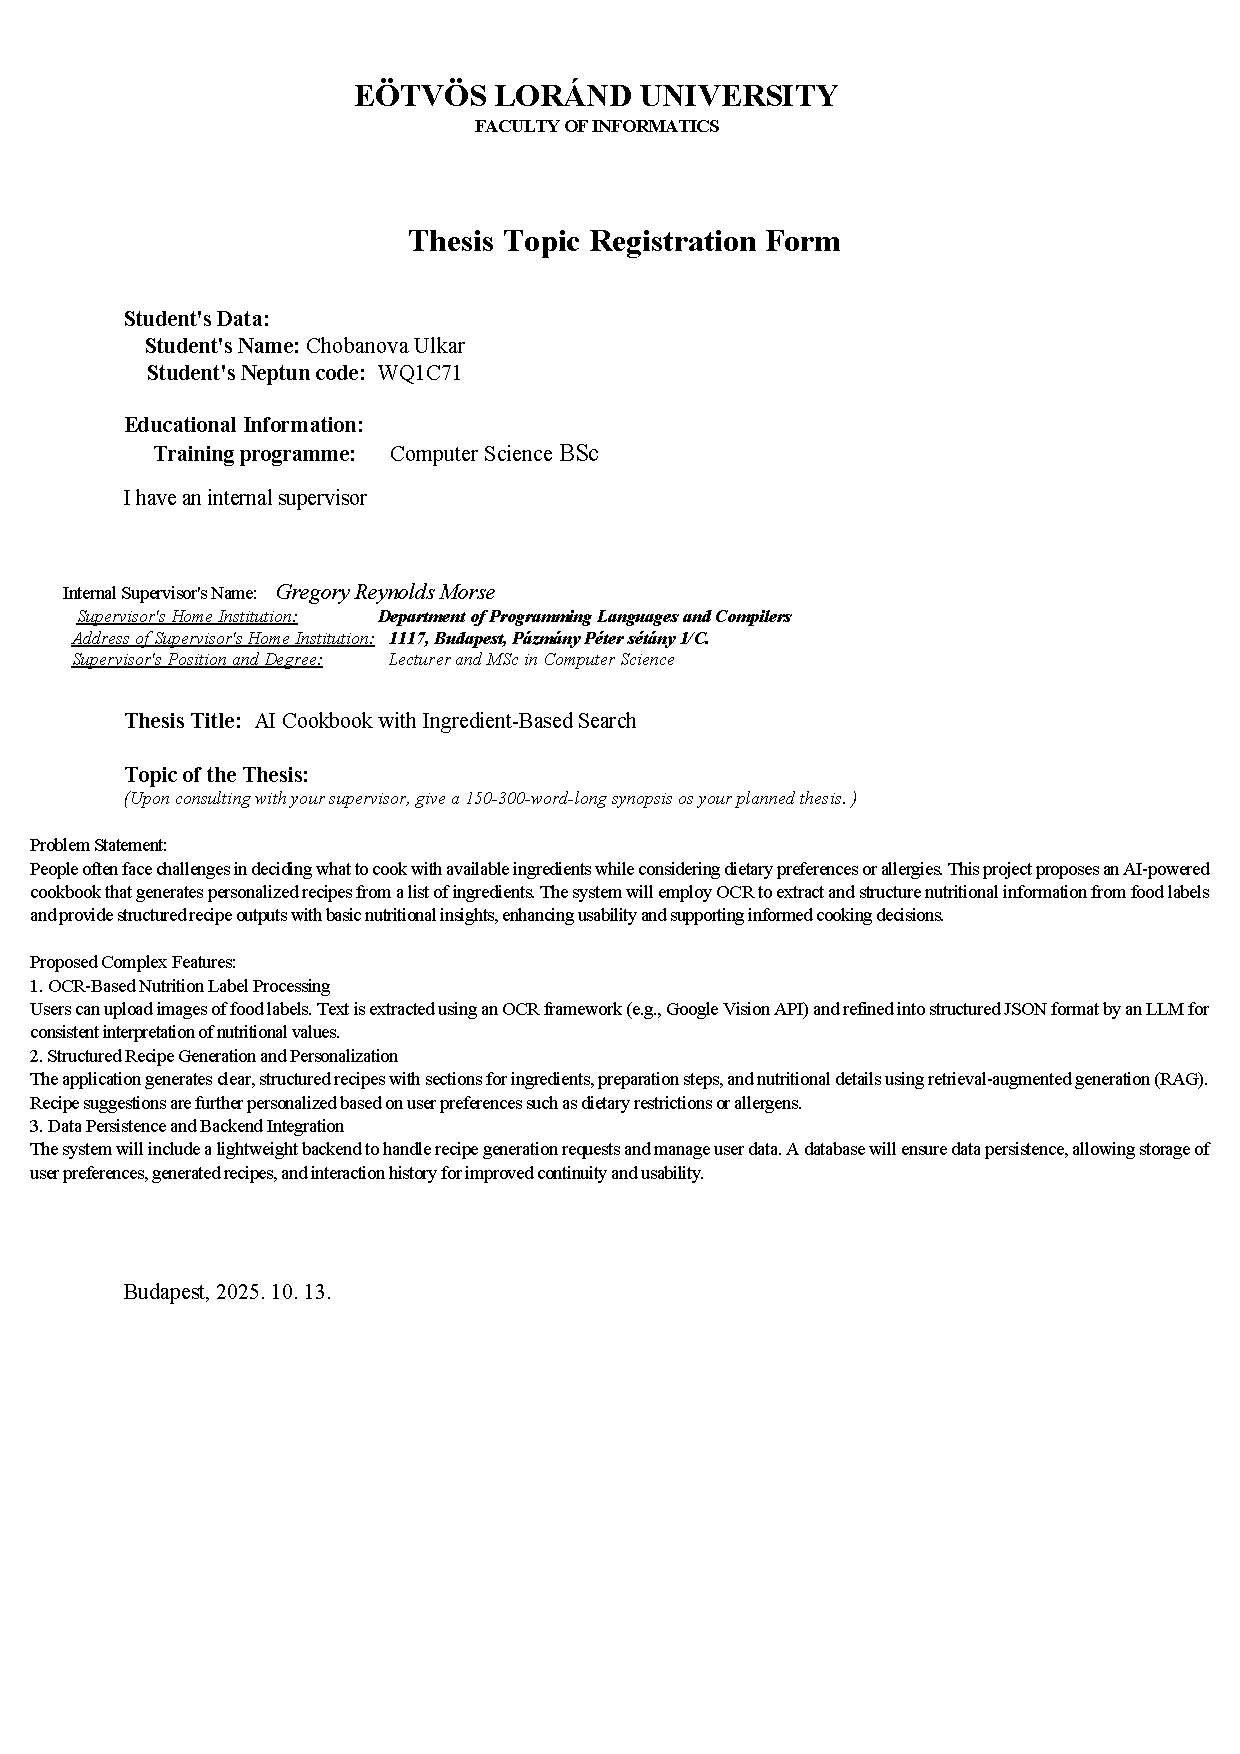
\includepdf[pages=1]{ApprovedThesisForm.pdf}

% Acknowledgements (optional)
\chapter*{\acklabel}
\addcontentsline{toc}{chapter}{\acklabel}
I would like to express my sincere gratitude to my supervisor,
Gregory Reynolds Morse, for his guidance, feedback, and continuous
support throughout the development of this thesis. I am also deeply
grateful to my family for their patience, encouragement, and constant
support during my studies and during the preparation of this work.
\cleardoublepage

% Table of contents (mandatory)
\tableofcontents
\cleardoublepage

% Main content
\chapter{Introduction}
\label{ch:intro}

\section{Motivation and Problem Statement}

Deciding what to cook from whatever ingredients happen to be available is a
common practical problem. Users typically know what is in their kitchen, but
translating that into a concrete, safe, and personalized meal requires browsing
multiple recipe websites, manually filtering results, and adapting instructions
to fit dietary restrictions or allergies. This process is repetitive and
effortful, yet users still often lack a simple tool that accepts a list of
ingredients and returns a structured recipe adapted to personal constraints.

A related inconvenience arises with packaged food products. Nutritional
information is printed on product labels in a format that is easy to read in
the moment but difficult to store, compare, or reuse digitally. Users who
want to track or inspect the nutritional content of packaged goods have no
practical way to capture that data without manually transcribing it, which
is both time-consuming and error-prone.

This thesis addresses both problems through a single integrated application.
The core feature allows users to submit a custom ingredient list along with
optional dietary preferences and allergy constraints, and receive a structured
recipe generated specifically from that input. A secondary feature accepts
an image of a food product label, extracts the printed nutritional text
automatically, and allows users to store the result in a structured digital form. Together,
these features form a coherent tool for ingredient-aware cooking decisions
and nutritional data capture within a single personalized cooking
assistant. 

\section{Goals and Objectives}

The main goal of the thesis is to deliver a working web application that
generates personalized recipes from user-provided ingredients and supports
OCR-based nutrition label processing. The project commits to four concrete
and verifiable objectives.

The first objective is to implement an ingredient-based recipe generation
workflow. The system accepts a list of ingredients and optional dietary
preferences and allergies, validates the request, and returns a structured
recipe containing a title, ingredient list, preparation steps, nutritional
estimate, and system warnings. To improve the relevance of generated
results, the workflow uses retrieval-augmented generation: before producing
a recipe, the system retrieves relevant entries from an indexed recipe corpus
and uses them as contextual grounding for the language model.

The second objective is to implement user-specific personalization and
persistence. Authenticated users can create accounts, save dietary
preferences and allergies, store generated recipes, and access both saved
recipes and their full generation history. This ensures the application
supports repeated and personalized use rather than one-time generation.

The third objective is to implement OCR-based nutrition label extraction.
The system accepts uploaded label images, validates and preprocesses them,
extracts text through an OCR provider, transforms the raw output into
structured nutritional fields, and allows authenticated users to save their
labels and extracted data.

The fourth objective is to implement and document the backend and data model
that support these workflows. This covers the system architecture, request
handling, authentication, persistent storage, media handling, and the
service boundaries required to coordinate recipe generation, OCR
processing, and history management.

\section{Scope and Constraints}

The scope of the thesis covers the implemented \emph{AI Cookbook with
Ingredient-Based Search} application and all features available in the final
system: ingredient-based recipe generation, preference- and allergy-aware
personalization, OCR-based nutrition label extraction, user authentication,
and storage of recipe and label history. It also covers the technical
documentation of the system, including the application architecture, main
request flows, persistent data model, and testing material.

The thesis does not aim to provide a general introduction to artificial
intelligence, nutrition science, or OCR theory beyond what is necessary to
explain the implemented solution.

Several constraints apply. Recipe generation, nutritional structuring, and
image generation depend on external AI services, meaning that response
quality and availability are not fully controlled by the local application.
OCR accuracy depends on the quality and readability of uploaded images.
Dietary preferences, allergy-related handling, and nutritional values
displayed by the system, whether extracted from labels or estimated for
generated recipes, are intended as application output for user guidance and
do not constitute certified dietary or medical advice.

The project also does not aim to provide production-grade infrastructure,
clinical nutritional analysis, or guaranteed factual correctness for every
AI-generated or OCR-derived value. Its purpose is to demonstrate a working
and well-documented implementation of the designed workflows within the
scope of a bachelor thesis.

The project is also constrained by its scope as a bachelor thesis. The
system was designed to be functionally complete and documentable within
limited development time. The thesis therefore focuses on the implemented
features and their software engineering realization rather than
production-scale concerns such as distributed deployment or expert-level
nutritional analytics. Additional feature expansion and broader
implementation improvements are therefore treated as future work.

\section{Thesis Roadmap}

Chapter 2 presents the user documentation and describes how the application
is configured, launched, and used from the perspective of its intended users.

Chapter 3 presents the developer documentation. It is divided into the
design, implementation, and testing sections, covering the software
requirements, system architecture, data model, implementation details,
and validation results of the application.

Chapter 4 concludes the thesis by summarizing the achieved results,
discussing the limitations of the current implementation, and outlining
directions for future improvement.

\cleardoublepage

\chapter{User documentation}
\label{ch:user}

This chapter documents the user-side aspects of the implemented
\emph{AI Cookbook with Ingredient-Based Search} application. It describes
how the system is prepared, configured, launched, and used in a
local thesis and development environment. It first presents the setup
and configuration steps required before the application can be used,
then documents the main workflows from the user's perspective. Because
the application integrates a FastAPI backend, a React frontend, a
local relational database, retrieval-based recipe generation, and
OCR-based nutrition label processing, proper initial setup is
required to ensure reliable execution of all workflows.

The chapter is organized into three sections. Section 2.1 outlines
the technical prerequisites and configuration steps, including
hardware and software requirements, dependency installation,
environment variables, and initial verification. Section 2.2
provides a user manual describing the main workflows, such as
recipe generation, personalization features, recipe storage, and
OCR-based food label extraction. Section 2.3 discusses known
issues, system limitations, and frequently asked questions based
on practical usage.

\cleardoublepage


\section{Installation, setup, and configuration guide}

This section describes the requirements and steps necessary to run
the application in a local development environment. It covers the
hardware and software prerequisites, required external services,
and the configuration steps needed before the backend, frontend,
database, vector store, and AI-supported features can be used.

\subsection{System requirements}

This subsection defines the conditions that should be satisfied
before the application is installed and executed in a local
development environment. Because the system combines a Python-based
backend, a React frontend, local persistent storage, and
multiple AI-supported services, successful operation depends on both
local development tools and external API access. The requirements
are therefore grouped into three categories: hardware requirements,
software requirements, and external service requirements.

\subsubsection{Hardware requirements}

\begin{itemize}
	\item \textbf{Operating system:} Windows~10 or newer, a recent Linux
	distribution, or a recent macOS version.
	\item \textbf{Processor:} Any modern 64-bit multi-core processor is
	sufficient for development and local execution.
	\item \textbf{Memory (RAM):} At least 8~GB is required, while 16~GB is
	recommended for smoother use when the backend, frontend, browser,
	and indexing-related tasks are active at the same time.
	\item \textbf{Storage:} At least 4~GB of free disk space is
	recommended. This covers the project source code, Python and Node.js
	dependencies, the local SQLite database, uploaded OCR images,
	generated recipe thumbnails, and the persisted Chroma vector store.
	\item \textbf{Internet connection:} Required during both setup and
	normal use. Dependency installation requires network access, and the
	AI-supported workflows depend on external APIs for recipe generation,
	embedding generation, OCR processing, and nutrition-data
	structuring.
\end{itemize}

\subsubsection{Software requirements}

\begin{itemize}
	\item \textbf{Python 3.11 or newer.} Required for the FastAPI backend,
	virtual environment management, dependency installation, Alembic
	database migrations, recipe indexing scripts, and backend testing.

	Download: \url{https://www.python.org/downloads/}.
	\item \textbf{Node.js and npm.} Required for installing frontend
	dependencies and running the React application through the Vite
	development server. A recent LTS version is recommended for local
	development.

	Download: \url{https://nodejs.org/en/download}.
	\item \textbf{Git.} Recommended for cloning, updating, and managing
	the repository in a reproducible way.

	Installation guide:\\
	\url{https://git-scm.com/book/en/v2/Getting-Started-Installing-Git}.
	\item \textbf{Modern web browser.} Required to access the frontend
	locally. Google Chrome, Mozilla Firefox, and Microsoft Edge are all
	suitable for development and normal use.
\end{itemize}

For platform-specific Python installation, interpreter usage, and
environment-management details, the official \emph{Python Setup and
Usage} guide can be consulted \cite{python2026setup}.

For platform-specific Node.js and npm installation details, the
official Node.js installation guide can be consulted
\cite{node2026setup}.

\subsubsection{External service requirements}

In addition to the local software stack, the AI-supported features
require access to two external services. The application can start
without these credentials, but the affected AI-supported workflows
will not function correctly until they are configured.

\textbf{OpenAI API access} is required for recipe generation,
embedding generation for the retrieval pipeline, structuring
OCR-extracted nutrition data into JSON, producing nutritional
estimates for generated recipes, and generating recipe thumbnail
images. For full local deployment, the application expects a valid
OpenAI API key to be provided through environment configuration by
the maintainer or developer operating the system. Ordinary end
users do not enter this value through the application interface.
Further information is
available at:
\par{\footnotesize\url{https://help.openai.com/en/articles/4936850-where-do-i-find-my-openai-api-key}}

\textbf{Google Cloud Vision credentials} are required for
OCR-based nutrition label extraction. The application expects
credentials to be provided through the
\texttt{GOOGLE\_APPLICATION\_CREDENTIALS} environment variable,
following the standard Google Cloud authentication flow. As with the
OpenAI key, these credentials are supplied during environment setup
by the maintainer or developer rather than by ordinary end users.
The authentication setup is described at:
\par
\url{https://cloud.google.com/vision/docs/authentication}.

\subsection{Getting the source code and installing dependencies}

This subsection explains how the project is obtained and how the
development dependencies are prepared for first use. The repository
contains a Python backend, a React frontend, migration files,
testing material, and thesis-related assets, so the complete project
root should be available locally before configuration begins.

The source code is hosted in a Git repository. Cloning the repository
is the preferred approach because it preserves the full project
structure and allows future updates to be pulled in a consistent way.
If the project is already available locally as a thesis submission
archive or extracted folder, the same setup steps can be followed from
that project root without cloning again.
The repository can be obtained with the following commands:

\lstset{caption={Cloning the project repository}, label=src:user-get-repo}
\begin{lstlisting}
git clone https://github.com/ulkarchbnv/ai-cookbook-thesis.git
cd ai-cookbook-thesis
\end{lstlisting}

After cloning, the project root should contain the main application
directories used during setup and development, most importantly
\texttt{backend}, \texttt{frontend}, \texttt{alembic}, and
\texttt{docs}. The
\texttt{backend} directory contains the FastAPI application and its
service logic, the \texttt{frontend} directory contains the React user
interface, and the \texttt{alembic} directory contains the database
migration files used to initialize and update the local schema. The
\texttt{docs} directory contains testing and evaluation material used
elsewhere in the thesis.

After the repository has been cloned, the backend environment should
be prepared first. The application uses Python for the backend, so it
is recommended to create a dedicated virtual environment in the
project root. This avoids interference with globally installed Python
packages and keeps the local setup reproducible.

\lstset{caption={Creating the Python virtual environment}, label=src:user-create-venv}
\begin{lstlisting}
python -m venv .venv
\end{lstlisting}

On Windows PowerShell, the virtual environment can be activated as
follows:

\lstset{caption={Activating the virtual environment in PowerShell}, label=src:user-activate-venv-win}
\begin{lstlisting}
.\.venv\Scripts\Activate.ps1
\end{lstlisting}

On Linux or macOS shells, the typical activation command is:

\lstset{caption={Activating the virtual environment on Linux or macOS}, label=src:user-activate-venv-unix}
\begin{lstlisting}
source .venv/bin/activate
\end{lstlisting}

Once the virtual environment is active, the backend requirements can
be installed from the dependency list stored in
\texttt{backend/requirements.txt}. This step installs the web
framework, database and migration libraries, AI-service client
libraries, OCR-related packages, retrieval-pipeline dependencies, and
project support tools such as the backend testing framework.

\lstset{caption={Installing backend dependencies}, label=src:user-install-backend}
\begin{lstlisting}
python -m pip install --upgrade pip
python -m pip install -r backend/requirements.txt
\end{lstlisting}

At this point, the backend runtime, database libraries, migration
tools, OCR-related dependencies, AI client libraries, and testing
packages are available inside the local virtual environment.

The frontend is maintained separately in the \texttt{frontend}
directory and must also be initialized before the application can be
started. Its dependencies are installed with \texttt{npm}, which
downloads the packages required for the React user interface, routing,
the Vite development server, and frontend tests.

\lstset{caption={Installing frontend dependencies}, label=src:user-install-frontend}
\begin{lstlisting}
cd frontend
npm install
cd ..
\end{lstlisting}

After both installation steps have finished, the local machine
contains all project files and package dependencies needed for the
next stage of setup. The environment is then ready for configuration
of the variables used by the backend and frontend services, which is
described in the following subsection.

\subsection{Environment configuration}

After the repository and package dependencies have been prepared, the
next step is to define the environment variables required by the
application. The backend loads its configuration from a
\texttt{.env} file located in the project root. The frontend reads its
API base URL through Vite environment handling, and in the current
implementation it also falls back to
\texttt{http://127.0.0.1:8000} when \texttt{VITE\_API\_BASE\_URL} is
not explicitly provided.

The project already provides a template file named
\texttt{.env.example}. This file should be copied to a new file named
\texttt{.env}, and the placeholder values should then be replaced
with valid local configuration values.

\lstset{caption={Creating the local environment file}, label=src:user-create-env}
\begin{lstlisting}
copy .env.example .env
\end{lstlisting}

On Linux or macOS, the equivalent command is typically:

\lstset{caption={Creating the local environment file on Linux or macOS}, label=src:user-create-env-unix}
\begin{lstlisting}
cp .env.example .env
\end{lstlisting}

The most important variables for local execution are the following:

\begin{itemize}
	\item \textbf{\texttt{OPENAI\_API\_KEY}} specifies the API key used by
	the recipe-generation, embedding, nutrition-structuring, and image
	generation features.
	\item \textbf{\texttt{GOOGLE\_APPLICATION\_CREDENTIALS}} points to the
	local path of the Google Cloud service-account JSON file used by the
	OCR provider.
	\item \textbf{\texttt{DATABASE\_URL}} defines the relational database
	connection. If this value is not overridden, the backend defaults to
	a local SQLite database file named \texttt{ai\_cookbook.db} in the
	project root.
	\item \textbf{\texttt{SECRET\_KEY}} is required for JWT creation and
	validation and must not be left empty.
	\item \textbf{\texttt{FRONTEND\_ORIGIN}} defines the allowed frontend
	origin for backend CORS handling. In the default local setup, this
	should match the Vite development server address.
\end{itemize}

In addition to these core values, the configuration file also
contains optional settings for model names, retrieval parameters,
upload limits, media directories, rate-limiting rules, and vector
store persistence paths. Many of these defaults are already suitable
for a standard local development setup, so they do not need to be
changed unless the deployment environment or experimental requirements
differ from the default configuration. However, required values such
as \texttt{SECRET\_KEY}, \texttt{OPENAI\_API\_KEY}, and, for OCR
usage, \texttt{GOOGLE\_APPLICATION\_CREDENTIALS}, must still be
configured explicitly.

If the frontend should target a backend address other than the default
\texttt{http://127.0.0.1:8000}, the \texttt{VITE\_API\_BASE\_URL}
variable can be provided through the frontend's Vite environment
configuration.

A typical local \texttt{.env} file follows the structure shown in
Code~\ref{src:user-env-example}. The values below are examples only
and should be replaced with valid credentials and paths. The example
is intentionally limited to the most important backend settings for a
standard local setup.

\lstset{caption={Example local environment configuration}, label=src:user-env-example}
\begin{lstlisting}
OPENAI_API_KEY=your_openai_key
OCR_PROVIDER=google_vision
GOOGLE_APPLICATION_CREDENTIALS=C:\path\to\your-google-service-account.json
DATABASE_URL=sqlite:///./ai_cookbook.db
SECRET_KEY=your_secret_key
ALGORITHM=HS256
FRONTEND_ORIGIN=http://localhost:5173
\end{lstlisting}

When this file has been created and updated, the backend can load its
runtime settings correctly, and the frontend can target the intended
local API endpoint.

\subsection{Verifying the installation}

Before launching the application, it is useful to verify that the
main tools and local files are available as expected. This helps
detect common setup mistakes early, such as a missing virtual
environment, an unavailable Node.js installation, or an incorrectly
named configuration file.

The first check is to confirm that the required command-line tools
are accessible and return valid version information.

\lstset{caption={Verifying the local toolchain}, label=src:user-verify-toolchain}
\begin{lstlisting}
python --version
node --version
npm --version
git --version
\end{lstlisting}

At this stage, Python should report version 3.11 or newer, while
Node.js and npm should also return installed versions without error.
Git is not required for runtime execution after cloning, but it
should still be available if the repository will be updated or
maintained locally.

The second check is to confirm that the expected local setup artifacts
exist in the project root. In a correctly prepared environment, the
repository should already contain the application source directories,
the \texttt{.venv} virtual environment directory, and the
\texttt{.env} configuration file.

\lstset{caption={Verifying key local files and directories}, label=src:user-verify-files}
\begin{lstlisting}
Get-ChildItem .venv, backend, frontend, alembic, .env
\end{lstlisting}

If these files and directories are present, the local installation can
be considered structurally complete. The next step is to initialize
the database and other local data resources required by the
application.

\subsection{Initializing the database and local retrieval data}

After the installation has been verified, the local data layer should
be initialized. In the default configuration, the backend uses a
SQLite database defined through \texttt{DATABASE\_URL}, and its schema
is managed through Alembic migration files located in the
\texttt{alembic} directory. Running the migration step ensures that
the required tables and indexes are created before the application is
started.

The migration command should be executed from the project root while
the Python virtual environment is active:

\lstset{caption={Applying database migrations}, label=src:user-run-migrations}
\begin{lstlisting}
alembic upgrade head
\end{lstlisting}

When this command completes successfully, the local database schema
contains the tables required for users, generated recipes, and saved
OCR extraction history. In the default SQLite-based setup, the file
\texttt{ai\_cookbook.db} is created automatically in the project root
if it does not already exist.

In addition to the relational database, the recipe-generation workflow
also depends on local retrieval data. The project already includes a
prepared recipe subset in \texttt{backend/data/recipes\_subset.json},
which serves as the source corpus for the retrieval-augmented
generation pipeline. This subset was prepared from the Food.com dataset
distributed through Kaggle. To make this corpus searchable, it must be
embedded and indexed into the local Chroma vector store.

\lstset{caption={Indexing the recipe corpus for retrieval}, label=src:user-index-recipes}
\begin{lstlisting}
python -m backend.scripts.index_recipes
\end{lstlisting}

This step reads the recipe subset, generates embeddings for the recipe
documents, and stores them in the Chroma persistence directory
specified by \texttt{CHROMA\_PERSIST\_DIRECTORY}. It should be executed
at least once before recipe generation is tested on a new local setup.

The project also includes a preparation script that can regenerate the
cleaned recipe subset when the raw dataset is available locally. For
normal local setup, however, this preprocessing step is not required
because the prepared subset used by the application is already
included in the repository.

Once the database migrations and vector-store indexing have both been
completed, the system is ready to launch the backend and frontend
services.

\subsection{Starting the backend and frontend}

After the local data layer has been initialized, the application can
be started. The backend and frontend run as separate development
services, so they are typically launched in two terminal windows.

The backend should be started first from the project root while the
Python virtual environment is active:

\lstset{caption={Starting the FastAPI backend}, label=src:user-start-backend}
\begin{lstlisting}
uvicorn backend.main:app --reload
\end{lstlisting}

In the default local configuration, the backend starts on
\texttt{http://127.0.0.1:8000}. If the startup is successful, the
terminal displays the Uvicorn server message and begins watching the
project files for code changes.

If a different host or port is needed, or if the backend must later be
deployed behind HTTPS with an SSL certificate, these operational details
should be taken from the official FastAPI deployment guide rather than
duplicated here \cite{fastapi2026deployment}.

The frontend is started separately from the \texttt{frontend}
directory:

\lstset{caption={Starting the React frontend}, label=src:user-start-frontend}
\begin{lstlisting}
cd frontend
npm run dev
\end{lstlisting}

In the default setup, the Vite development server starts on
\texttt{http://localhost:5173}. The frontend sends its API requests to
the backend URL defined by \texttt{VITE\_API\_BASE\_URL}, which should
therefore match the backend address used during startup.

When both services are running, the application can be opened in a web
browser by visiting the frontend address. The backend exposes the API
used by the user interface, while the frontend provides access to the
pages for recipe generation, nutrition label extraction, saved items,
history, and account management.

\subsection{Post-startup verification}

After both services have been started, a short smoke test should be
performed before the full user workflows are exercised. The purpose of
this check is not detailed feature validation, but quick confirmation
that the local setup is operational.

The backend can be checked by opening
\texttt{http://127.0.0.1:8000/} in a browser. In a successful setup,
the service returns a small JSON response containing the message
\texttt{"AI Cookbook backend is running"}.

The frontend can be checked by opening
\texttt{http://localhost:5173}. In a successful setup, the home page
of the application is displayed and the main navigation bar is visible.
It should then be possible to open the \textbf{Generate} and
\textbf{Food Labels} pages without an immediate runtime error.

Once this smoke test succeeds, the local setup can be considered
complete and the application is ready for functional use. The
following section describes the user workflows supported by the
system.

\section{User manual}

This section describes how the application is used after the local
environment has been configured and both services are running. The
manual covers both the first-use path through the application and the
main workflows available from the implemented user interface. It is
based on the actual frontend structure of the system and focuses on
the features that are most important from the user perspective:
accessing the system, managing an account, generating recipes,
processing food labels, and reviewing saved or historical results.

Although recipe generation can be used without authentication,
creating an account unlocks the persistence features of the system.
Authenticated users can store dietary preferences and allergy
defaults, save generated recipes, and keep a history of both recipe
generation and OCR-based food label extraction.

\subsection{Quick-start walkthrough from launch to first meaningful action}

This subsection provides a short first-use path through the
application. Its purpose is to help a new evaluator or user reach a
meaningful result quickly after startup, without yet exploring every
feature in detail.

Once the backend and frontend have been started as described in the
previous section, the application is opened at
\texttt{http://localhost:5173}. The home page appears first and gives
access to the two main workflows of the system: recipe generation and
food-label extraction.

The quickest meaningful action is recipe generation as a guest user.
The user opens the \textbf{Generate} page, enters a comma-separated
list of ingredients such as \texttt{chicken, rice, onion}, and submits
the form with the \textbf{Generate Recipe} button. If the backend is
configured correctly and the required AI services are available, the
page returns a structured recipe containing a title, ingredients,
preparation steps, a nutrition estimate, and any warning messages.
This confirms that the main backend, retrieval, and frontend response
flow is operational.

An alternative first-use path is the OCR-based workflow. The user
opens the \textbf{Food Labels} page, selects an image of a nutrition
label, and clicks \textbf{Extract Nutrition}. A successful response
returns both raw OCR text and structured nutrition data. This confirms
that file upload, OCR processing, and AI-assisted structuring are all
working.

If the user wants to test persistence features as part of the initial
exploration, the next step is to open the \textbf{Login} page, create
an account, and log in. After authentication, generated recipes can be
saved, profile defaults can be configured, and recipe or OCR history
becomes available.

\subsection{Feature-by-feature guide with annotated key screens}

This subsection presents the main screens of the implemented user
interface one by one. Each screenshot is accompanied by a short
textual annotation describing the most important visible areas and the
user actions supported on that screen.

\subsubsection{Home page and basic navigation}

When the frontend is opened in the browser, the application displays
the home page. This page functions as the main entry point and gives
the user a concise overview of the system. It introduces the three
main capabilities of the application: recipe generation,
OCR-supported nutrition label extraction, and data persistence.

The page also provides two primary call-to-action buttons:

\begin{itemize}
	\item \textbf{Generate a Recipe}, which opens the recipe-generation
	page.
	\item \textbf{Scan a Food Label}, which opens the OCR-based nutrition
	label page.
\end{itemize}

At the top of the interface, the navigation bar provides access to the
main pages of the system:

\begin{itemize}
	\item \textbf{Home} returns to the landing page.
	\item \textbf{Generate} opens the recipe-generation workflow.
	\item \textbf{Food Labels} opens the nutrition label extraction page.
	\item \textbf{Saved} displays recipes that have been explicitly saved
	by the authenticated user.
	\item \textbf{History} displays the user's generated recipe history,
	including unsaved entries.
	\item \textbf{Login} or \textbf{Account} opens the authentication and
	profile-management page.
\end{itemize}

If the user is already authenticated, the navigation bar also displays
a \textbf{Logout} button. This immediately removes the stored session
token on the client side and returns the application to guest mode.

The main visible areas of the screen are the headline section, the two
primary action buttons, and the top navigation bar. Together, these
elements guide the user toward either the recipe-generation or OCR
workflow and provide access to the rest of the application. This layout
is shown in Figure~\ref{fig:user-home-page}.

\begin{figure}[H]
	\centering
	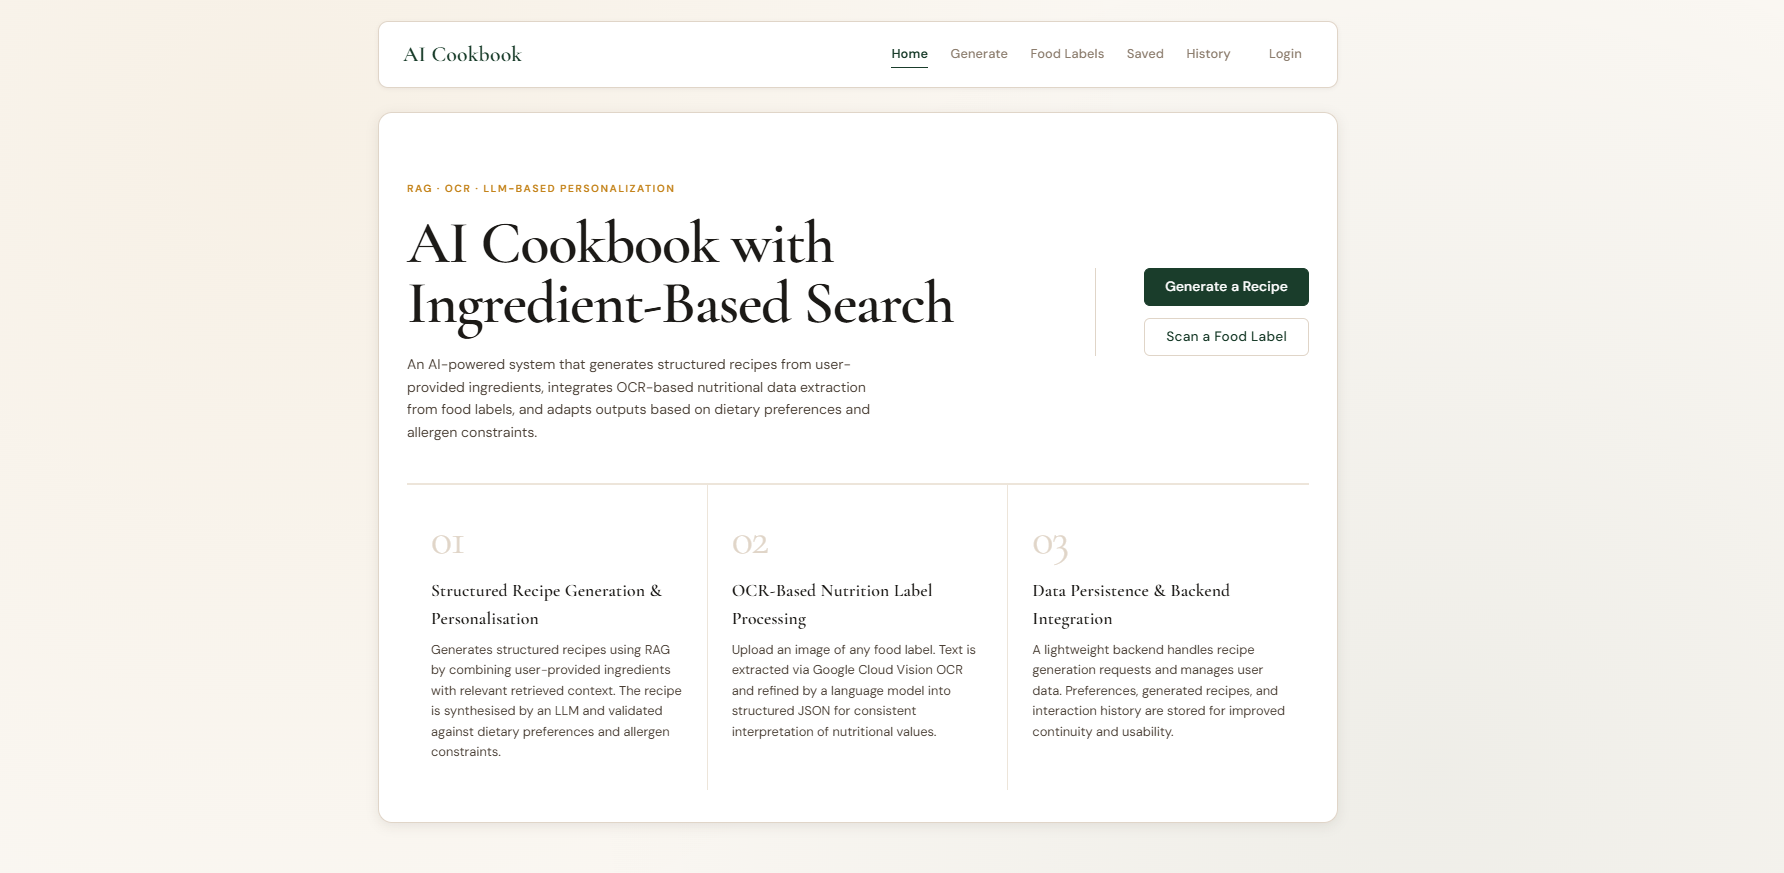
\includegraphics[width=0.9\textwidth]{images/HomePage.png}
	\caption{Home page of the AI Cookbook application}
	\label{fig:user-home-page}
\end{figure}

\subsubsection{Account creation, login, and profile defaults}

The \texttt{/login} page serves both as the authentication page for
guest users and as the account-management page for authenticated
users. Before login, the page presents two tabs: \textbf{Login} and
\textbf{Sign Up}. This allows a new user to create an account without
leaving the page. The guest-facing authentication view is shown in
Figure~\ref{fig:user-login-page}.

\begin{figure}[H]
	\centering
	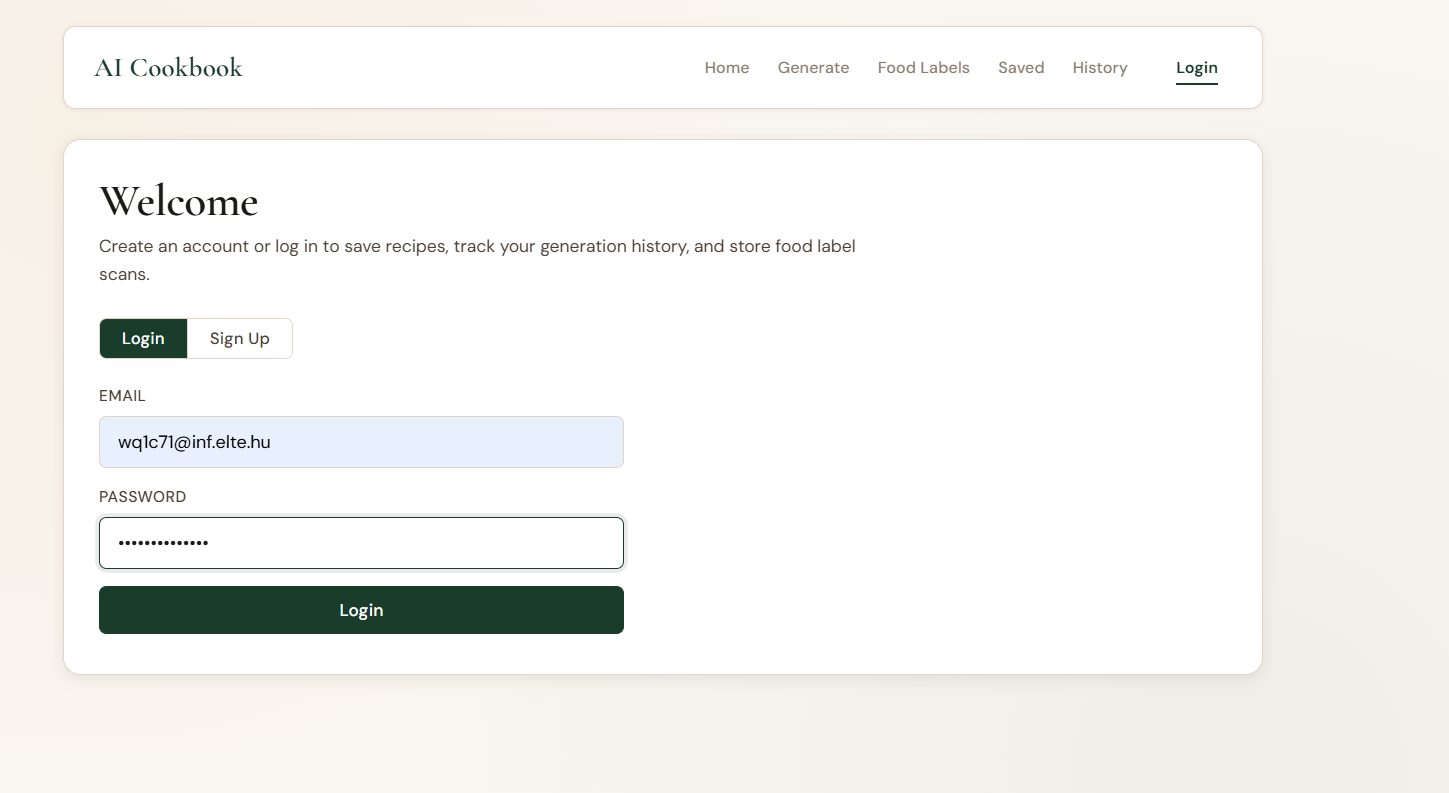
\includegraphics[width=0.82\textwidth]{images/Login.png}
	\caption{Login and registration page}
	\label{fig:user-login-page}
\end{figure}

To register a new account, the user switches to the \textbf{Sign Up}
tab, enters an email address and password, and submits the form. If
the email address is not already registered, the system creates the
account and returns a confirmation message. The user can then switch
back to the login tab and authenticate with the same credentials.

To log in, the user enters the registered email address and password
and submits the login form. On successful authentication, the backend
returns a JWT access token. The frontend stores this token locally and
uses it automatically in subsequent authenticated requests.

After login, the same page changes into an account-management view.
Instead of the login form, the user sees a summary of the current
profile data:

\begin{itemize}
	\item the account email address,
	\item the saved list of dietary preferences,
	\item the saved list of allergies.
\end{itemize}

Below the profile summary, the page provides a form for updating
default dietary preferences and allergy values. These defaults are
important because they can be reused later on the recipe-generation
page. If the user leaves the optional preference and allergy fields
empty during recipe generation, the application automatically falls
back to the saved profile values.

This makes the account page an important bridge between authentication
and later personalized recipe-generation behavior, because the values
stored here directly affect future requests when the user relies on
saved defaults.

The key visible parts of this screen are the tab selector, the
credential form, and, after login, the profile summary and update
form. This page therefore functions both as the entry point for
authentication and as the place where personalization defaults are
maintained. The authenticated account-management view is shown in
Figure~\ref{fig:user-account-page}.

\begin{figure}[H]
	\centering
	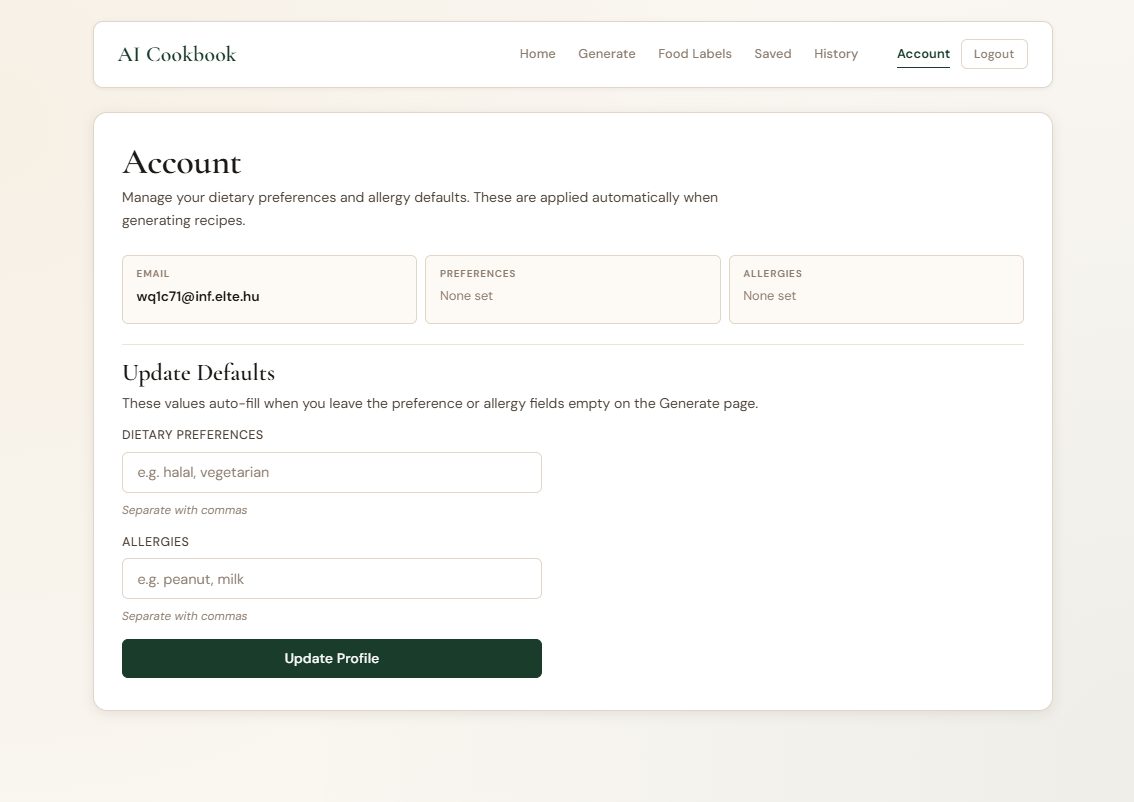
\includegraphics[width=0.82\textwidth]{images/Account.png}
	\caption{Account page after login, showing saved dietary defaults}
	\label{fig:user-account-page}
\end{figure}

\subsubsection{Recipe generation}

The recipe-generation page is the main workflow of the application.
The user enters a comma-separated list of available ingredients and
may optionally specify dietary preferences and allergies. If the user
is already authenticated and has saved default preferences or allergy
values in the account page, these defaults are applied automatically
when the optional fields are left empty.

After the form is submitted, the frontend sends the request to the
backend recipe-generation endpoint. The backend validates the input,
retrieves relevant recipe context from the indexed corpus, invokes the
language model, and returns a structured response. The result page
shows the generated recipe title, ingredient list, any additional
ingredients that may be required, preparation steps, a nutrition
estimate, and warning messages where applicable.

The screen is organized around three main areas: the input form, the
recipe result card, and the save action shown for authenticated users.
This makes it possible to move directly from ingredient entry to
inspection of the returned recipe and, when logged in, to persistence
of the result. The implemented screen is shown in
Figure~\ref{fig:user-generate-recipe}.

If the recipe was generated while the user was logged in, the page
also offers a \textbf{Save Recipe} action. This stores the generated
recipe in the user's saved collection and also preserves it in the
generation history.

\begin{figure}[H]
	\centering
	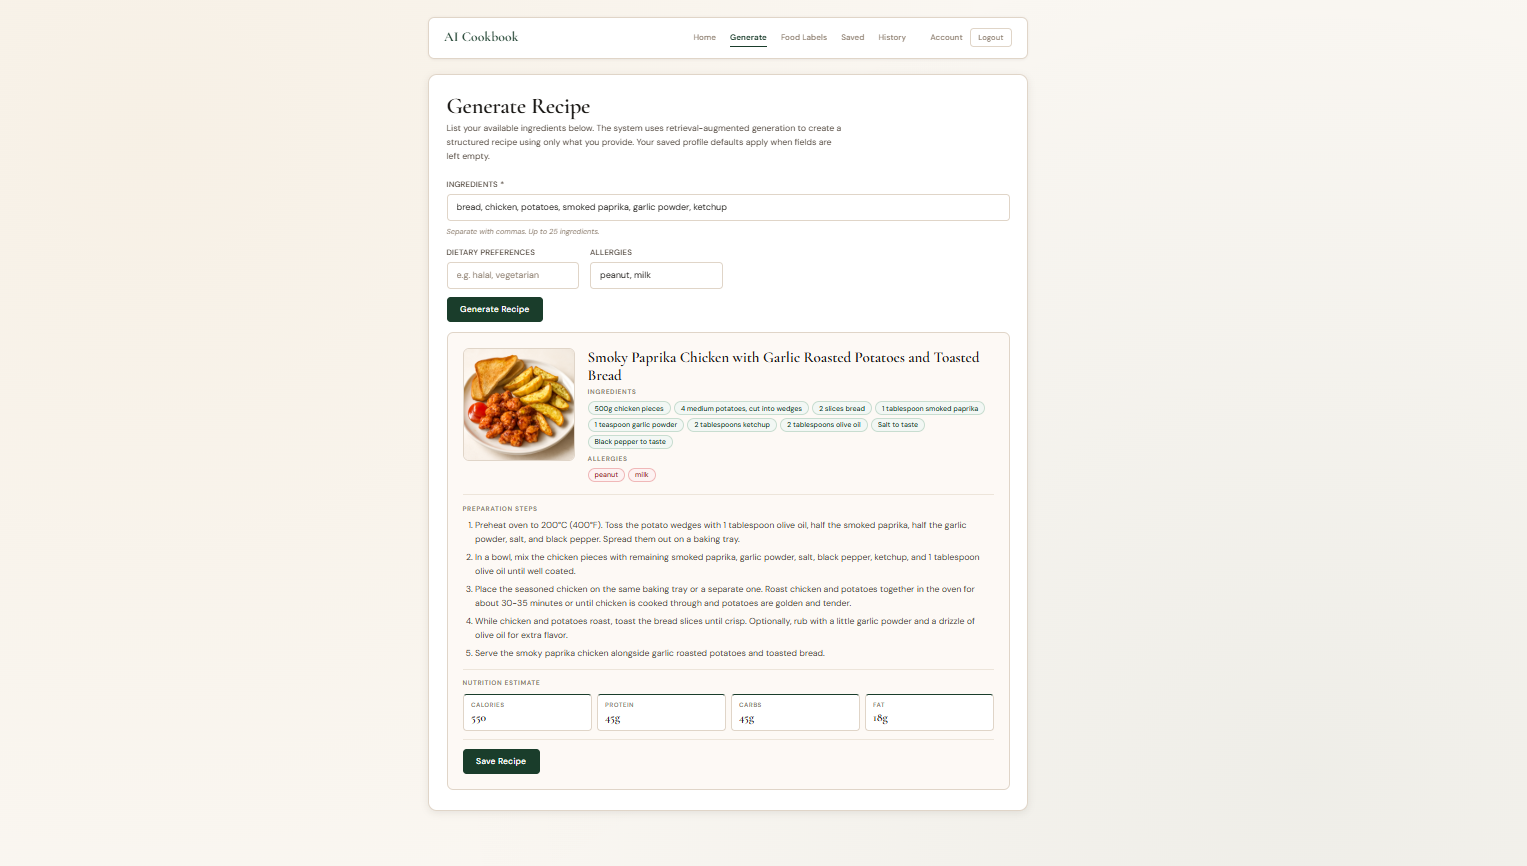
\includegraphics[width=0.9\textwidth]{images/GenerateRecipe.png}
	\caption{Recipe-generation page with a generated result}
	\label{fig:user-generate-recipe}
\end{figure}

\subsubsection{Food label extraction}

The \textbf{Food Labels} page provides the OCR-based nutrition-label
workflow. The user selects an image file containing a food label and
submits it for processing. The page first shows a local preview of the
selected image, then displays the extracted structured nutrition
values together with the raw OCR text returned by the backend.

If the user is logged in, the extracted result can be saved to the
personal label history. Saved entries remain available on the same
page and can be browsed with pagination when multiple records exist.
For unauthenticated users, extraction is still available, but
persistent storage is disabled.

The main visible regions on this page are the upload area, the
extraction result block, and the saved label history shown for
authenticated users. This page therefore combines immediate OCR usage
with later review of previously saved extraction results. The screen is
shown in Figure~\ref{fig:user-ocr-page}.

\begin{figure}[H]
	\centering
	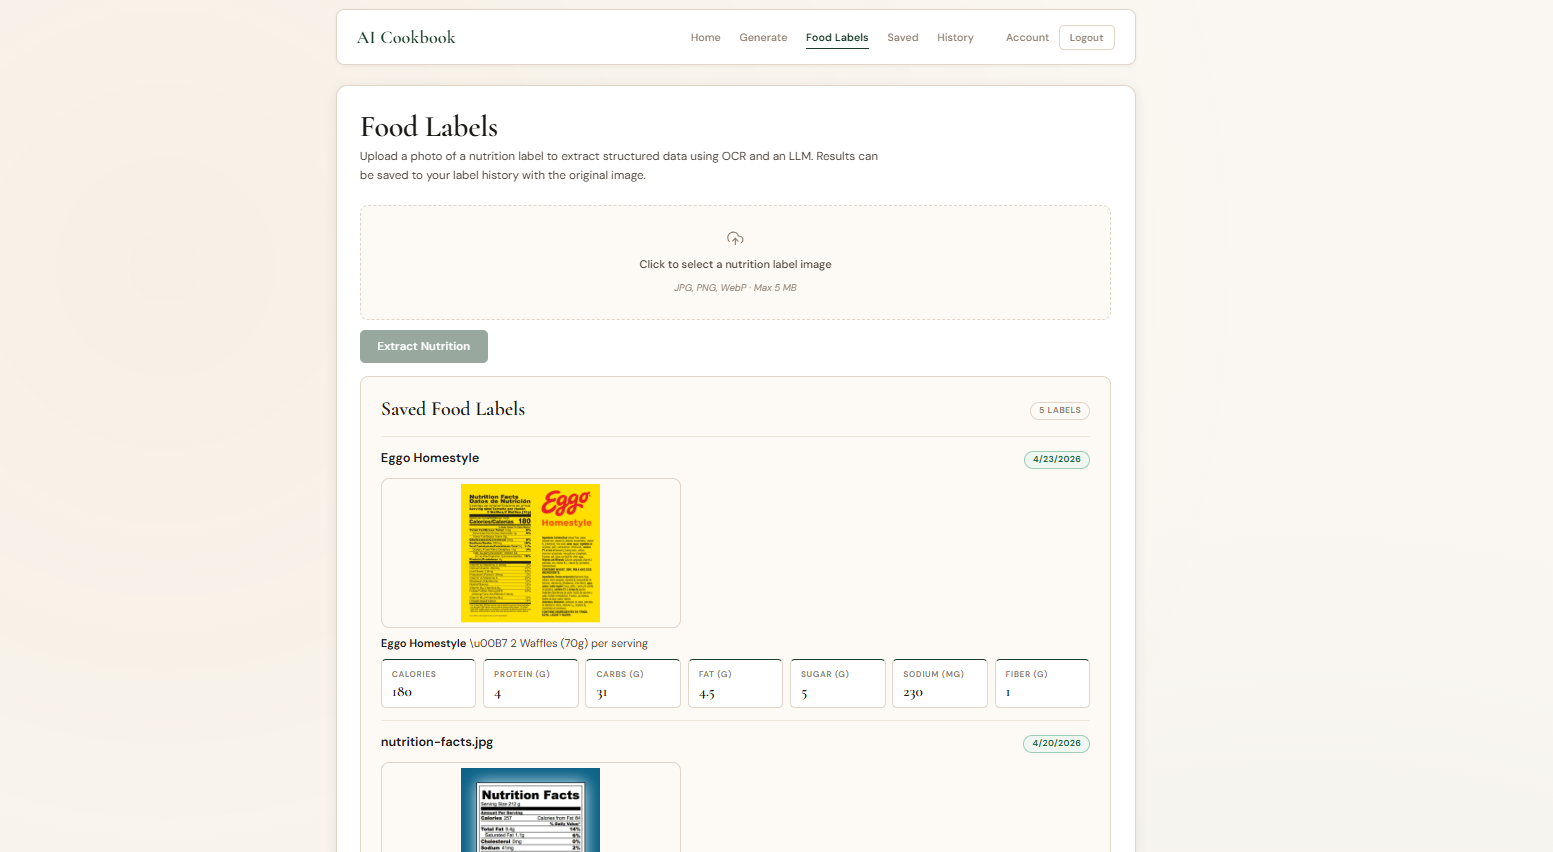
\includegraphics[width=0.9\textwidth]{images/OCR.png}
	\caption{Food label extraction page with OCR result}
	\label{fig:user-ocr-page}
\end{figure}

\subsubsection{Saved recipes}

The \textbf{Saved} page lists recipes that the authenticated user has
explicitly bookmarked after generation. Each entry is displayed as a
card containing the recipe title, key ingredients, optional
preferences and allergy markers, and the date on which the recipe was
saved.

The cards can be expanded interactively to reveal the preparation
steps and nutrition estimate. If the user is not logged in, the page
does not display private content and instead instructs the visitor to
authenticate first.

The key visible elements are the list of saved recipe cards, the saved
date indicator, and the expandable details section. This keeps the
page focused on compact review first and detailed inspection only when
requested by the user. The page is shown in
Figure~\ref{fig:user-saved-recipes}.

\begin{figure}[H]
	\centering
	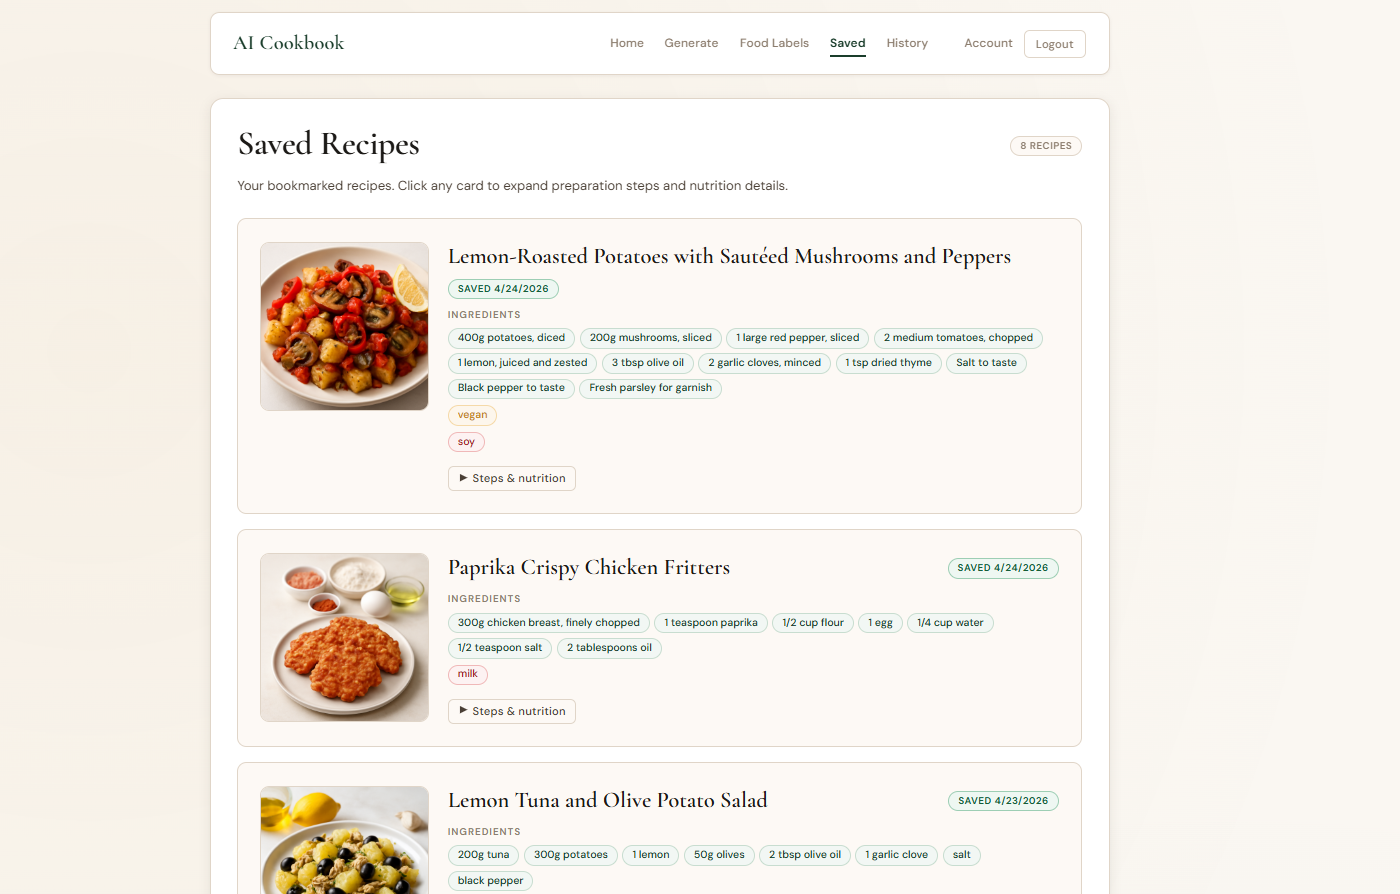
\includegraphics[width=0.9\textwidth]{images/SavedRecipes.png}
	\caption{Saved recipes page}
	\label{fig:user-saved-recipes}
\end{figure}

\subsubsection{Recipe history}

The \textbf{History} page provides a broader view than the saved
recipes page. It includes every recipe generated by the authenticated
user, including entries that were not explicitly saved. This makes the
page useful for reviewing previous outputs, comparing generated
results, and returning to earlier recipe ideas.

Each history card shows whether the recipe is merely generated or also
saved, along with the creation timestamp and any warning messages
returned during generation. As on the saved recipes page, each card
can be expanded to display the preparation steps and nutrition
estimate in full detail.

The visible structure of the page emphasizes recipe status, creation
time, and warning information, so that the user can distinguish
quickly between temporary and explicitly saved outputs before opening
the full details. The page is shown in
Figure~\ref{fig:user-recipe-history}.

\begin{figure}[H]
	\centering
	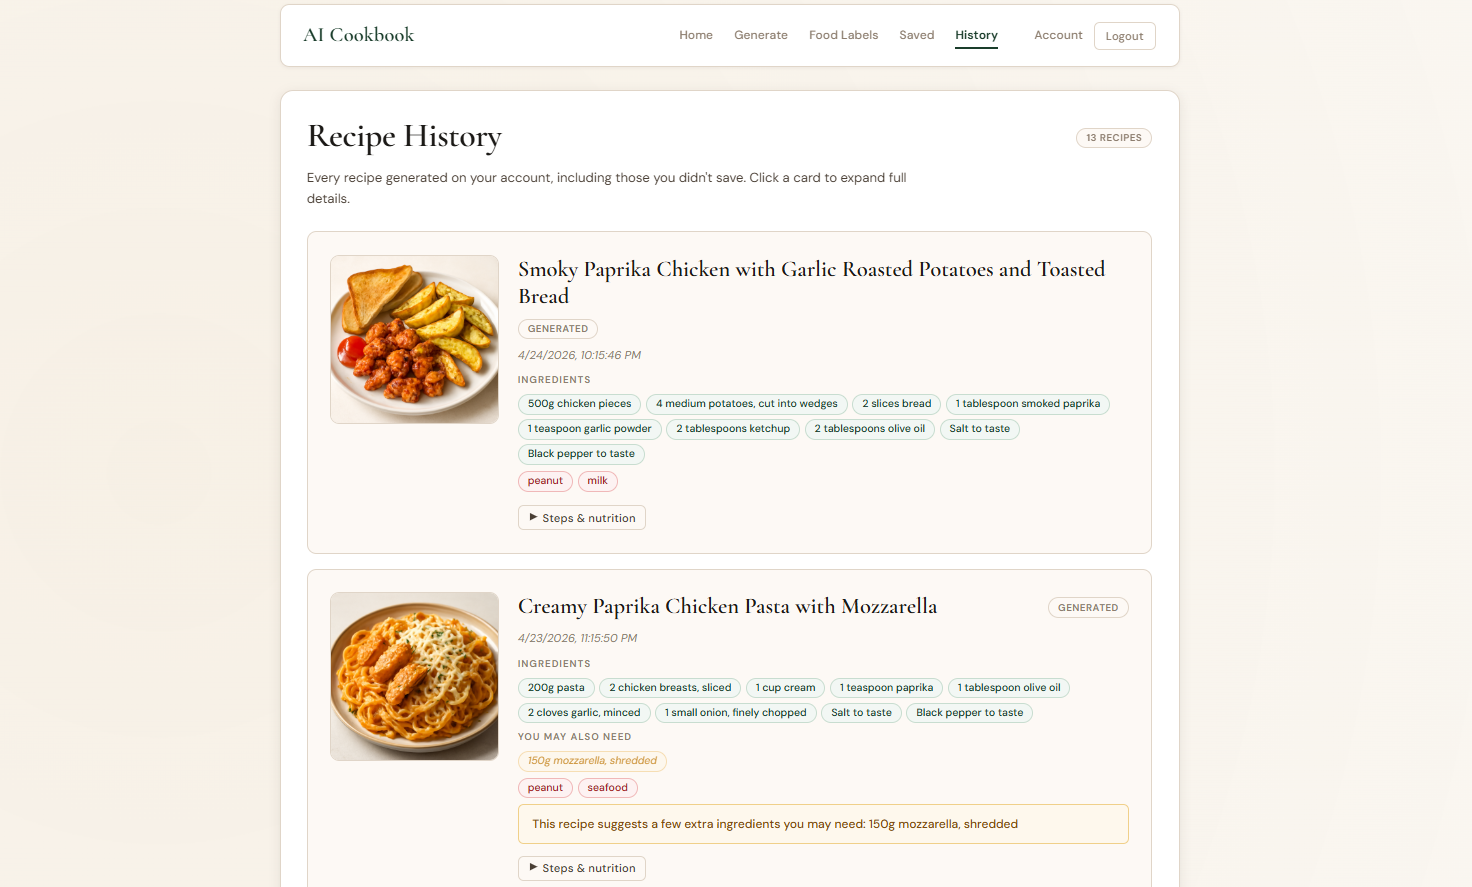
\includegraphics[width=0.9\textwidth]{images/History.png}
	\caption{Recipe history page}
	\label{fig:user-recipe-history}
\end{figure}

\subsection{Step-by-step workflows for the main features}

This subsection collects the most important multi-step workflows of the
application in a task-oriented format. These workflows correspond to
the main interactive features promised by the project and implemented
in the final system.

\subsubsection{Creating an account and setting profile defaults}

\begin{enumerate}
	\item Open the \textbf{Login} page from the navigation bar.
	\item Select the \textbf{Sign Up} tab.
	\item Enter a valid email address and password, then submit the form.
	\item Return to the \textbf{Login} tab and authenticate with the same
	credentials.
	\item After login, review the account summary shown on the same page.
	\item Enter dietary preferences and allergies in the update form and
	save the changes.
\end{enumerate}

After this workflow, the profile contains stored defaults that can be
reused during recipe generation when the optional preference and
allergy fields are left empty.

\subsubsection{Generating a recipe from ingredient input}

\begin{enumerate}
	\item Open the \textbf{Generate} page.
	\item Enter a comma-separated ingredient list.
	\item Optionally enter dietary preferences and allergies, or leave
	these blank to use the saved profile defaults when authenticated.
	\item Click \textbf{Generate Recipe}.
	\item Review the returned title, ingredients, additional ingredients,
	preparation steps, nutrition estimate, and any warning messages.
\end{enumerate}

This is the core workflow of the application and demonstrates the
interaction between frontend input, backend validation, retrieval, and
LLM-based recipe synthesis.

\subsubsection{Saving a generated recipe and reviewing it later}

\begin{enumerate}
	\item Log in before generating the recipe.
	\item Complete the recipe-generation workflow on the
	\textbf{Generate} page.
	\item Click \textbf{Save Recipe} in the result area.
	\item Open the \textbf{Saved} page to verify that the recipe appears
	in the saved collection.
	\item Open the \textbf{History} page to verify that the same recipe
	also appears in the generation history.
\end{enumerate}

This workflow demonstrates the persistence behavior of the
application. Saved recipes remain accessible from the dedicated saved
collection, while all generated recipes remain visible in the broader
history view.

\subsubsection{Extracting nutrition data from a food label}

\begin{enumerate}
	\item Open the \textbf{Food Labels} page.
	\item Select an image containing a readable nutrition label.
	\item Submit the extraction request with
	\textbf{Extract Nutrition}.
	\item Review the extracted structured nutrition fields and the raw
	OCR text returned by the backend.
\end{enumerate}

This workflow exercises the upload, preprocessing, OCR, and
AI-assisted structuring path of the system.

\subsubsection{Saving an OCR extraction for later access}

\begin{enumerate}
	\item Log in before or after a successful extraction.
	\item Complete the nutrition-label extraction workflow.
	\item Click \textbf{Save to Food Labels}.
	\item Verify that the extraction appears in the saved label history
	on the same page.
	\item If multiple saved entries exist, use the pagination controls to
	browse them.
\end{enumerate}

This workflow shows the persistence and later review path for
OCR-derived nutrition data.

\subsection{Accessibility, localisation, and access notes}

This subsection summarizes practical usage characteristics that affect
how different users can access the system.

\textbf{Access control.} The application does not implement multiple
user roles such as administrator, editor, or moderator. The effective
access model is binary: guest or authenticated user. Guests can use
the recipe-generation and OCR-extraction workflows, but
persistence-related features are restricted to authenticated users.
Saved recipes, recipe history, and saved OCR history are therefore
user-scoped features.

\textbf{Localisation.} The implemented user interface is available in
English only. No runtime language-switching or multilingual interface
layer is currently implemented.

\textbf{Accessibility.} The interface uses standard web form controls,
buttons, and page navigation patterns. The file-selection area on the
OCR page also supports keyboard-triggered activation through the
implemented \texttt{Enter} and \texttt{Space} handlers. However, the
project does not currently include a dedicated accessibility settings
panel, screen-reader-specific optimization layer, or a formal
accessibility compliance evaluation. Accessibility improvements are
therefore a reasonable area for future development.

\section{Troubleshooting, limitations, and frequently asked questions}

This section summarizes the most important practical limitations of
the application and collects the issues that a user is most likely to
encounter during local use. Because the system depends on external AI
services and local configuration, not every problem is caused by
the frontend interface itself. In many cases, unsuccessful operation
can be traced back to missing credentials, service availability,
or incomplete local setup.

\subsection{Known issues and recommended workarounds}

\textbf{The frontend loads, but requests fail immediately.}
This usually indicates that the backend service is not running or that
\texttt{VITE\_API\_BASE\_URL} does not match the actual backend
address. The user should confirm that the FastAPI backend is running
on the expected port and that the frontend environment points to the
same API base URL.

\textbf{Login or signup fails unexpectedly.}
If account-related requests fail, the backend should be checked first.
The database migrations may not have been applied yet, or the
\texttt{SECRET\_KEY} required for token creation may be missing from
the environment configuration.

\textbf{Recipe generation returns an error.}
Recipe generation depends on the OpenAI API key and on the retrieval
index prepared from the local recipe corpus. If the API key is
missing, invalid, or rate-limited, the request may fail. The same can
happen if the recipe corpus has not yet been indexed into the Chroma
vector store.

\textbf{OCR extraction fails or returns poor output.}
This may happen when the uploaded image is blurred, poorly cropped,
rotated, too large, or contains limited readable text. OCR extraction
also depends on valid Google Cloud Vision credentials, so incorrect
credential paths can prevent the feature from working at all.

\textbf{Recipe generation rejects the request even though ingredients
were entered.}
This can happen when all provided ingredients conflict with the chosen
allergy settings or dietary preferences. In that case, the backend
rejects the request rather than generating an unsafe recipe. The
recommended workaround is to remove the conflicting ingredients or
adjust the selected dietary constraints.

\textbf{Saving features are unavailable.}
Saving recipes and OCR extraction results requires authentication. A
guest user can still generate a recipe or process a food label, but
the persistent save actions remain disabled until the user logs in.

\textbf{Recipe thumbnail generation is missing for an otherwise valid
recipe.}
The recipe-generation workflow attempts to attach an image thumbnail,
but thumbnail generation depends on an external image-generation API.
If that request fails, the backend still returns the generated recipe
without an image and adds a warning message instead. In practice, the
recommended workaround is simply to retry the request later, while
treating recipe generation itself as the primary feature and the
thumbnail as an optional enhancement.

\textbf{An authenticated session appears to be lost after a restart or
after token expiry.}
The frontend stores the access token locally and reloads the user
profile at application startup. If the token is no longer valid, the
frontend clears it and returns to guest mode. The recommended
workaround is to log in again. Since the application does not
implement refresh tokens or server-side session management, this is
expected behavior of the current implementation.

\subsection{System and functional limitations}

The application is intended as a functional AI-assisted cooking and
nutrition tool, but it also has clear limitations that should be
understood by the user.

\begin{itemize}
	\item \textbf{AI output is not guaranteed to be perfect.} Generated
	recipes, nutritional estimates, OCR-structured values, and
	generated thumbnails all depend on external AI services. The quality
	of these outputs may vary between requests.
	\item \textbf{Nutritional values are approximate.} The nutrition
	estimate attached to generated recipes is intended for guidance only.
	It should not be treated as a certified nutritional analysis.
	\item \textbf{Dietary filtering is rule-based rather than
	medically comprehensive.} The application handles allergies and
	preferences through keyword-based restrictions and prompt-level
	controls, which improves safety but does not replace expert dietary
	validation.
	\item \textbf{OCR accuracy depends heavily on image quality.} Clear,
	well-lit, and correctly oriented label images produce better
	results than low-resolution or visually noisy inputs.
	\item \textbf{OCR image persistence is best-effort rather than
	guaranteed.} During OCR extraction, the system attempts to store the
	uploaded label image before processing it. However, if that media-write
	step fails, the OCR workflow may still continue and return a
	successful structured nutrition result. In such cases, the extraction
	can still be used, but the saved history entry may not include a
	usable stored-image reference.
	\item \textbf{The software does not provide medical, clinical, or
	certified dietary decision support.} Neither generated recipes nor
	extracted nutrition values should be treated as medically verified
	output.
	\item \textbf{The software does not support editing or deleting saved
	content.} In the current implementation, users can create accounts,
	update profile defaults, generate recipes, save recipes, and save OCR
	extractions, but there is no interface for removing or editing saved
	recipes or saved OCR history entries after they have been stored.
	\item \textbf{The software does not implement advanced account
	management features.} There is no email verification, password-reset
	workflow, refresh-token support, or multi-role authorization model.
	\item \textbf{Recipe images are optional enhancements rather than
	guaranteed outputs.} A generated recipe can still be valid and usable
	even if no thumbnail image is attached. When image generation is
	unavailable, the system returns the recipe itself and treats the
	missing thumbnail as a secondary issue.
	\item \textbf{Recipe history and saved recipes are not the same
	thing.} The \textbf{History} page contains all generated recipe
	entries for the authenticated user, while the \textbf{Saved} page
	contains only the subset that was explicitly saved. Users should
	expect these two views to differ.
	\item \textbf{Saved OCR results are shown separately from saved
	recipes.} Food-label extractions do not appear on the main
	\textbf{Saved} page. They remain available on the \textbf{Food
	Labels} page under the saved OCR history section.
\end{itemize}

\subsection{Frequently asked questions from realistic usage scenarios}

\textbf{Can the application be used without creating an account?}
Yes. Guests can generate recipes and use food-label OCR extraction.
However, saved recipes, recipe history, saved food labels, and profile
defaults require authentication.

\textbf{Why does the recipe sometimes include additional ingredients?}
The recipe-generation workflow prioritizes the provided ingredients,
but it may introduce a small number of extra ingredients when the
language model determines that a practical recipe would otherwise be
incomplete. These extra items are shown separately in the result.

\textbf{Why do saved preferences appear even when I leave the fields
empty on the Generate page?}
If the user is authenticated, the system automatically reuses the
saved dietary preferences and allergy defaults from the account page
when the optional fields are left blank.

\textbf{Do I need to re-index the recipe corpus every time I start the
project?}
No. The indexing step is normally required only for the initial local
setup, or when the recipe corpus has changed and the retrieval index
needs to be regenerated.

\textbf{Are the OCR results stored automatically?}
No. OCR extraction and OCR saving are separate actions. The user must
explicitly choose to save the extraction result if persistent history
is desired.

\textbf{Why can I generate recipes as a guest, but I cannot save them?}
The application separates feature access from persistence. Recipe
generation and OCR extraction are available without authentication, but
any data that is stored per user account requires login so that it can
be associated with a specific user.

\textbf{Why does the Saved page not show food-label results?}
Saved recipes and saved OCR extractions are stored separately in the
current implementation. Recipes appear on the \textbf{Saved} and
\textbf{History} pages, while saved food-label results are shown in the
\textbf{Food Labels} page under the saved label history section.

\textbf{Why does the same recipe sometimes show the same thumbnail even
after changing dietary options?}
The current thumbnail cache is derived mainly from the ingredient list.
This reduces repeated image-generation cost, but it may cause visually
similar requests to reuse the same cached image even when dietary
preferences differ.

\textbf{Why was my recipe request rejected after I selected allergies or
dietary preferences?}
If every provided ingredient conflicts with the selected restrictions,
the system refuses the request instead of generating an unsafe result.
In practice, this means at least one safe ingredient must remain after
filtering for recipe generation to continue.

\cleardoublepage

\cleardoublepage
\chapter{Developer Documentation}
\label{ch:design}

This chapter documents the technical contribution of the thesis through
three implemented thesis contributions. The first contribution is an
OCR-based nutrition-label processing workflow that accepts uploaded
food-label images, extracts text, and converts the result into a
structured nutritional representation. The second contribution is a
structured recipe-generation and personalization workflow that combines
ingredient-based input, retrieval-augmented generation, and user
constraints such as dietary preferences and allergens. The third
contribution is the backend and persistence layer that integrates these
workflows into one application, supports authenticated use, and stores
user-specific data such as preferences, generated recipes, and OCR
history.

The rest of the chapter explains these contributions from three
perspectives. The design section presents the planned structure and
responsibilities of the system, the implementation section shows how
that design was realized in code, and the testing section evaluates the
resulting application behavior.

\cleardoublepage

\section{Design}
\label{sec:design}

This section presents the design of the \emph{AI Cookbook with
Ingredient-Based Search} system. The goal of the design is not to
repeat implementation details, but to explain how the system was
structured before discussing concrete modules and code in the later
implementation section. The design had to cover three core concerns of the project:
user-facing interaction, backend application logic, and persistent
data management.

The system solves two closely related problems. First, it helps users
generate recipes from available ingredients while respecting dietary
preferences and allergy constraints. Second, it extracts structured
nutrition data from food-label images so that the user does not need
to transcribe labels manually. These two features share the same
application shell, authentication model, and persistence layer, but
they differ in workflow shape: recipe generation is a retrieval- and
generation-oriented pipeline, while OCR is an image-processing and
information-extraction pipeline. The design therefore emphasizes clear
separation between routes, services, providers, and storage.

\subsection{Design Drivers and Requirements}

\subsubsection{Design goals and principles}

The design of the system is guided by a small set of principles that
reflect the actual risks and responsibilities of an AI-assisted cooking
application.

\begin{itemize}
	\item \textbf{Safety-oriented generation.} Allergy and dietary
	constraints should influence validation, retrieval, prompt
	construction, output checking, and warning generation instead of being
	treated as decorative metadata.
	\item \textbf{Explainability and transparency.} The system should make
	AI-supported decisions visible through warnings, excluded ingredients,
	raw OCR text, and structured nutrition output rather than hiding them
	behind a black-box interface.
	\item \textbf{Modularity.} Routes, services, providers, persistence
	models, and frontend task pages should remain separated by
	responsibility so that changes in one subsystem do not force unrelated
	rework elsewhere.
	\item \textbf{Reproducibility.} The application should be rebuildable
	from versioned source, migrations, dependency manifests, environment
	settings, and indexing scripts, which is important both for thesis
	evaluation and for repeatable local deployment.
	\item \textbf{User trust.} Users should be able to understand what was
	generated, what was inferred, and what limitations still apply. In
	this project, trust is built through predictable workflows and visible
	evidence rather than through stylistic polish alone.
\end{itemize}

These principles shape the rest of the design chapter. The requirements,
workflows, architecture, data model, and user interface all follow the
same priorities, so the chapter remains focused on one system instead
of reading as a set of separate technical topics.

\subsubsection{System purpose}

The application is designed as an interactive web system rather than a
single-run AI script. Users should be able to move between recipe
generation, OCR-based nutrition extraction, account management, and
history views through a stable browser interface. The backend is
responsible for validating requests, enforcing ownership rules,
orchestrating AI-supported workflows, and persisting user-specific
results.

From a design perspective, the most important objective is controlled
workflow execution. The application accepts user input that can be
unsafe or incomplete, and it also depends on external AI services that
may return imperfect outputs. For that reason, the design does not
treat generation as a single black-box API call. Instead, it introduces
validation, filtering, retrieval, output checking, optional retry, and
selective persistence as explicit stages.

\subsubsection{Primary actors and major use cases}

The system has two human-facing roles and one external-service role.

\begin{itemize}
	\item \textbf{Guest user.} Can generate recipes and run OCR
	extraction, but cannot persist private data.
	\item \textbf{Authenticated user.} Can use the guest-level functions
   and can also manage profile defaults, save recipes, and browse recipe
   and OCR history.
	\item \textbf{External AI services.} Provide text generation,
	embeddings, OCR text extraction, and recipe-image generation.
\end{itemize}

The main user-visible use cases are registration, login, profile
update, recipe generation, recipe saving, browsing saved recipes,
browsing recipe history, OCR extraction, and OCR result saving. The
table below lists only external actors; the backend itself is part of
the system and is discussed later in the architecture section.

\par\bigskip

\begin{table}[H]
	\centering
	\scriptsize
	\begin{tabular}{|p{3.1cm}|p{10.8cm}|}
		\hline
		\textbf{Actor} & \textbf{Responsibilities} \\
		\hline
		Guest user & Provides ingredients or nutrition-label images, triggers recipe generation and OCR extraction, reviews returned results, and explores the application without private persistence features. \\
		\hline
		Authenticated user & Owns guest capabilities and additionally manages stored profile defaults, saves generated recipes, browses recipe history, and persists OCR extraction history under a private account scope. \\
		\hline
		External AI services & Supply embeddings, recipe generation, recipe-thumbnail generation, and OCR text extraction through provider-facing interfaces used by the backend workflows. \\
		\hline
	\end{tabular}
	\caption{Actors and responsibilities in the AI Cookbook system}
	\label{tab:actors-responsibilities}
\end{table}

\begin{figure}[H]
	\centering
	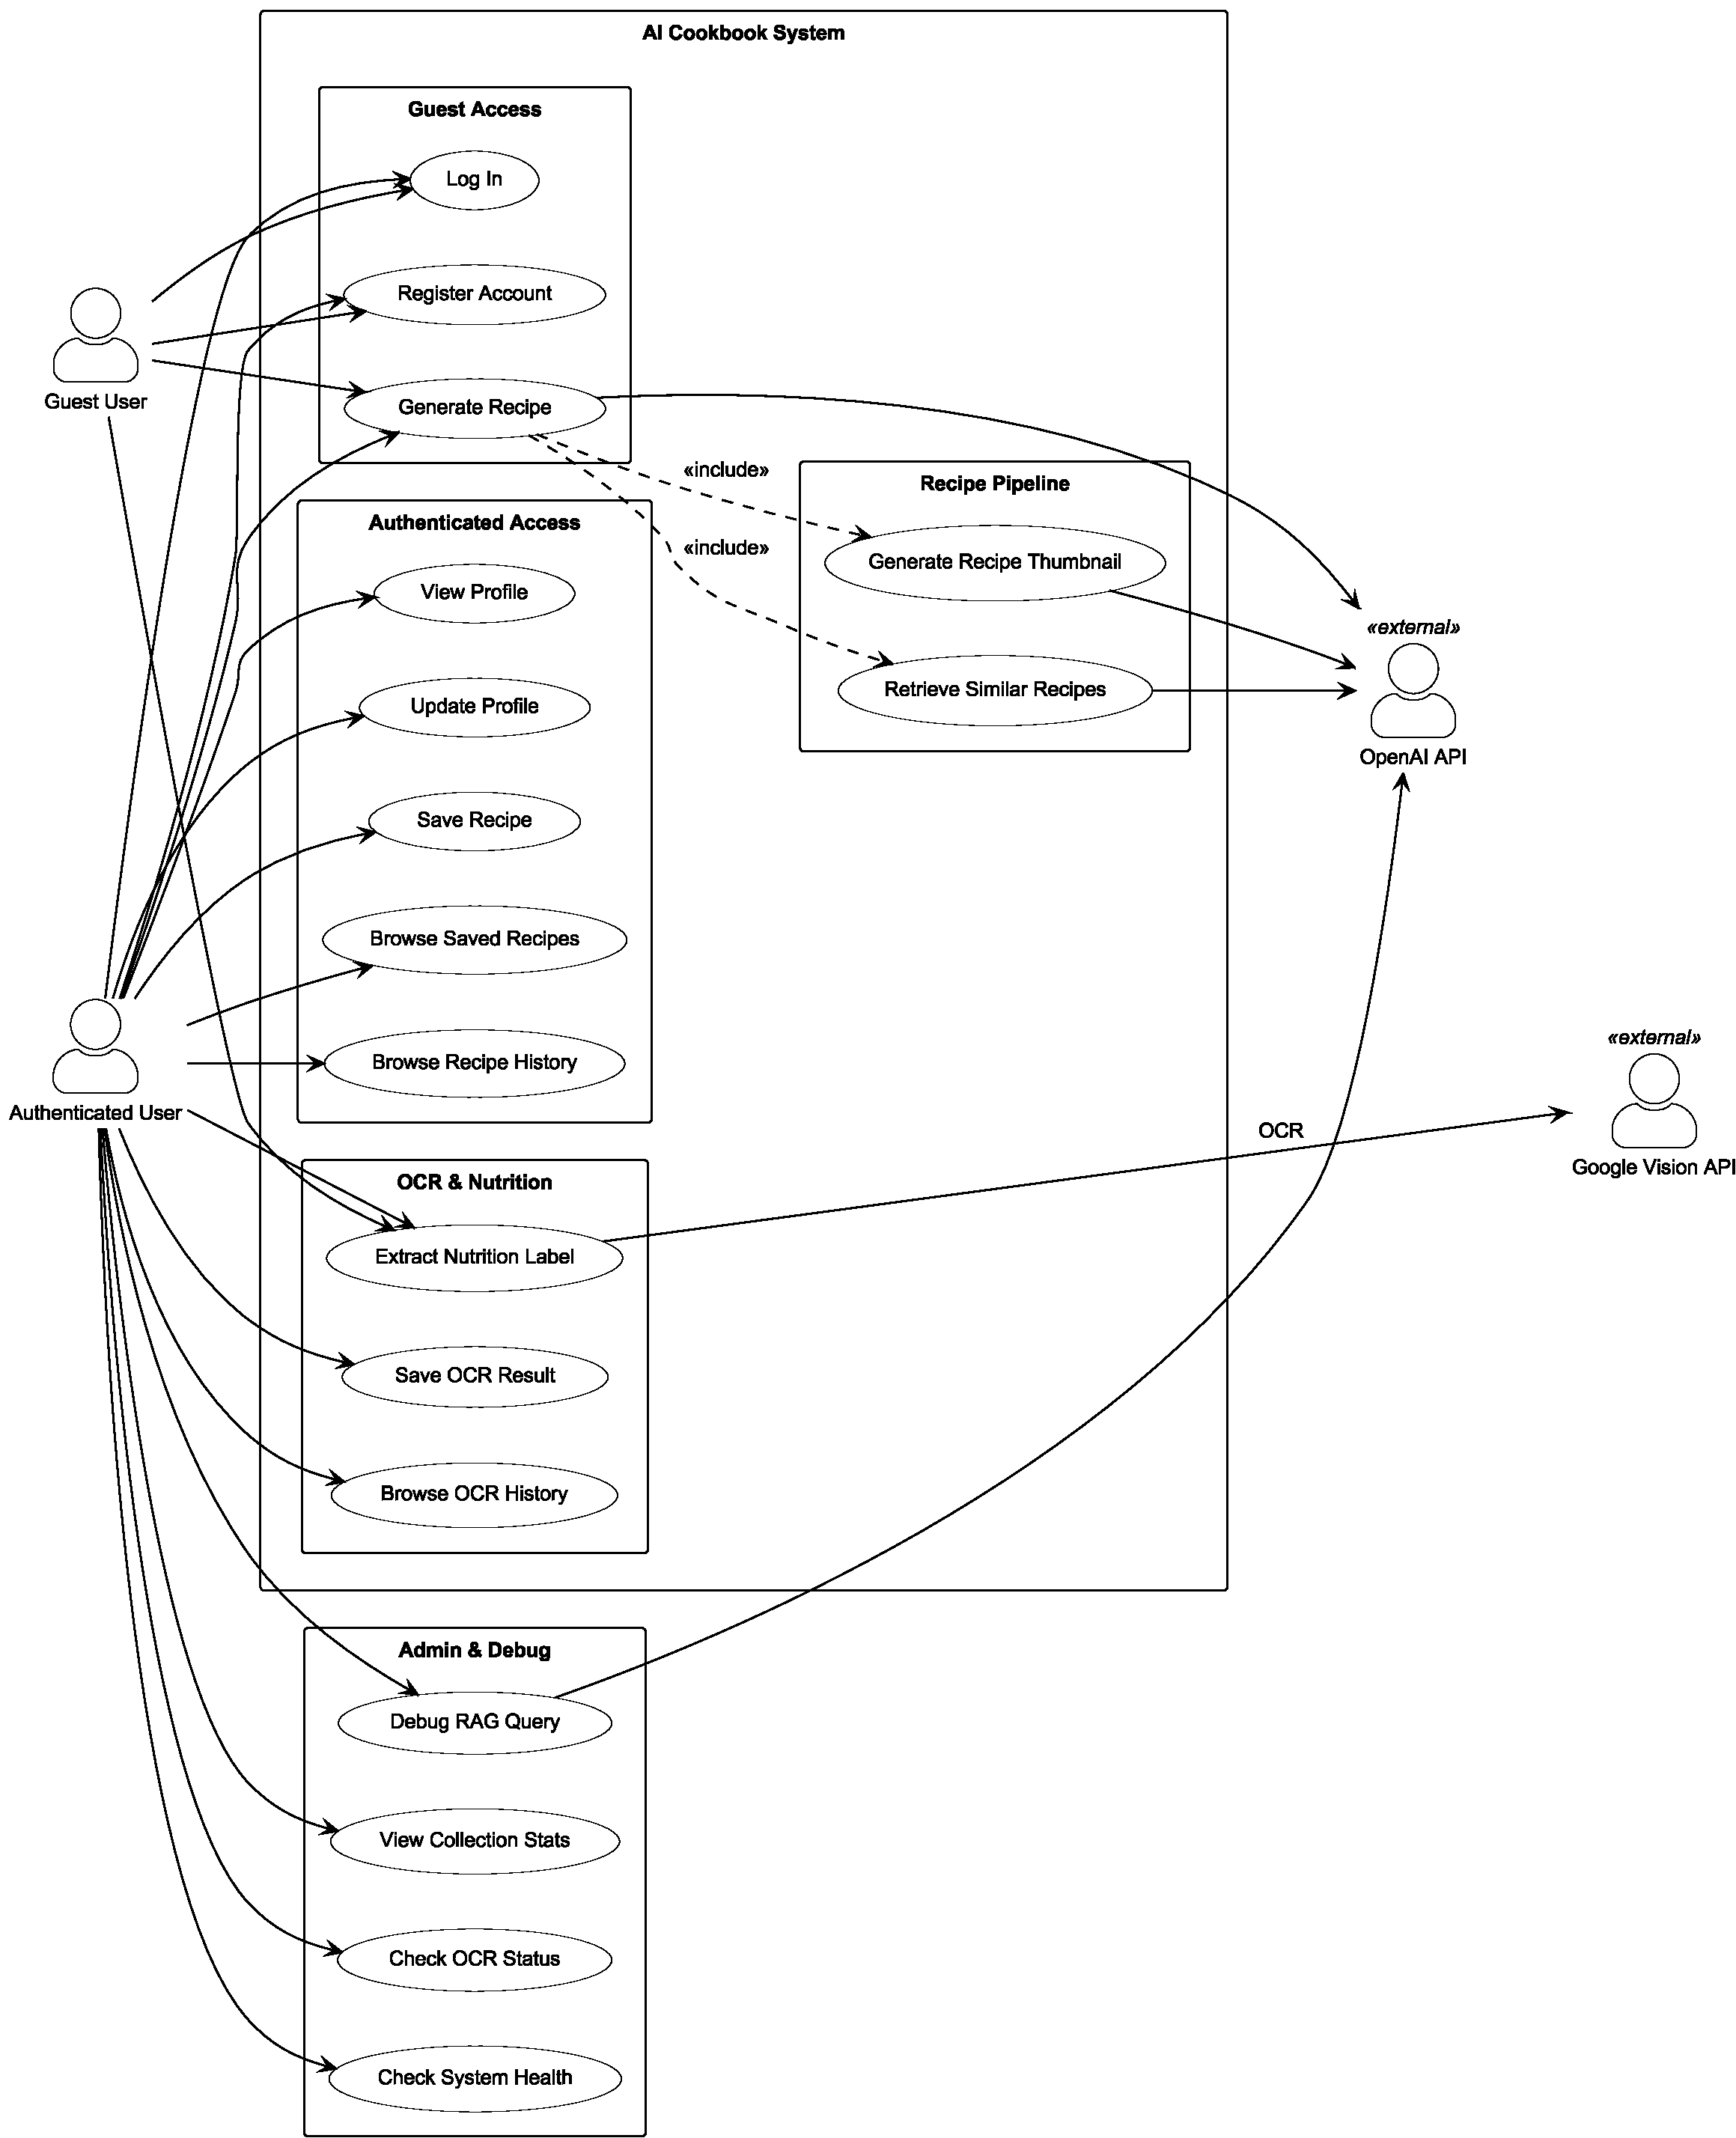
\includegraphics[width=\textwidth]{images/use-case-diagram.pdf}
	\caption{Use case diagram of the main user-visible system functions}
	\label{fig:design-use-case}
\end{figure}

\subsubsection{Functional requirements}

The main functional requirements of the system are the following.

\begin{enumerate}
	\item \textbf{FR-1: Ingredient-based recipe generation.} The system
	shall accept a non-empty ingredient list and return a structured
	recipe containing a title, ingredient list, preparation steps, and a
	nutrition estimate.
	\item \textbf{FR-2: Preference- and allergy-aware generation.} The
	system shall allow the request to include dietary preferences and
	allergy constraints, and these constraints shall influence the recipe
	generation workflow.
	\item \textbf{FR-3: Retrieval-grounded generation.} Before recipe
	generation, the system shall retrieve relevant recipe context from an
	indexed recipe corpus and use that context to ground the language
	model.
	\item \textbf{FR-4: User authentication.} The system shall support
	user registration, login, and retrieval of the current authenticated
	profile.
	\item \textbf{FR-5: Profile defaults.} The system shall allow
	authenticated users to store dietary preferences and allergies as
	profile defaults.
	\item \textbf{FR-6: Recipe history.} The system shall persist generated
	recipes for authenticated users and make them available through a
	history view.
	\item \textbf{FR-7: Explicit recipe saving.} The system shall allow an
	authenticated user to mark a generated recipe as saved and display
	saved recipes separately from full history.
	\item \textbf{FR-8: OCR extraction.} The system shall accept a food
	label image, validate it, extract raw text, and return structured
	nutrition fields.
	\item \textbf{FR-9: OCR history.} The system shall allow authenticated
	users to save OCR results and later browse those extractions through a
	history view.
	\item \textbf{FR-10: Protected ownership.} The system shall ensure that
	saved recipes, generation history, OCR history, and profile data are
	visible only to the owning authenticated user.
\end{enumerate}

The design makes these requirements testable through explicit input
limits, response-shape guarantees, and route behavior. Those measurable
criteria are summarized in Table~\ref{tab:design-fr-criteria}.

\begin{table}[H]
	\centering
	\scriptsize
	\begin{tabular}{|p{1.4cm}|p{5.7cm}|p{7.2cm}|}
		\hline
		\textbf{ID} & \textbf{Requirement focus} & \textbf{Acceptance criterion derived from the design} \\
		\hline
		FR-1 & Recipe request and response structure & A recipe request contains 1--25 ingredients; each ingredient string is at most 80 characters after trimming. A successful response contains a title, ingredient list, step list, and nutrition estimate object. \\
		\hline
		FR-2 & Constraint-aware generation & Preference and allergy lists may each contain at most 10 entries. Ingredients conflicting with declared allergies or dietary preferences are excluded before generation and surfaced as warnings in the response. \\
		\hline
		FR-3 & Retrieval grounding & For every recipe request, the backend queries the vector store for up to 10 candidates, filters unsafe matches, ranks the remainder, and forwards the best 3 contexts to the generation prompt. \\
		\hline
		FR-4 & Authentication lifecycle & The system exposes dedicated signup, login/token, and current-user profile retrieval routes. Passwords are never stored in plaintext, and authenticated identity is reconstructed from a signed JWT. \\
		\hline
		FR-5 & Profile defaults & The authenticated user can persist default preferences and allergies, and those values are returned as part of the profile representation. \\
		\hline
		FR-6 & Recipe history & When the requester is authenticated, every successful recipe generation creates a history row owned by that user. History listing is paginated with page size in the range 1--50. \\
		\hline
		FR-7 & Explicit saving & Saving a recipe requires authentication and a valid \texttt{generated\_recipe\_id} owned by the current user. The operation sets \texttt{is\_saved} and records \texttt{saved\_at}. \\
		\hline
		FR-8 & OCR extraction pipeline & OCR upload accepts common image formats, rejects empty uploads, enforces a maximum size of 5\,242\,880 bytes and a maximum of 20\,000\,000 pixels, then returns both raw OCR text and structured nutrition fields. \\
		\hline
		FR-9 & OCR history & Saved OCR results are persisted only for authenticated users and listed through a paginated history endpoint with page size in the range 1--50. \\
		\hline
		FR-10 & Ownership protection & Recipe save/list/history and OCR save/history queries are always filtered by the authenticated user identifier, so one user's records are not visible to another. \\
		\hline
	\end{tabular}
	\caption{Measurable acceptance criteria for the functional requirements}
	\label{tab:design-fr-criteria}
\end{table}

\subsubsection{Non-functional requirements}

The design also had to satisfy several non-functional requirements.

\begin{enumerate}
	\item \textbf{NFR-1: Usability.} The main workflows should be
	discoverable through a small and stable set of pages.
	\item \textbf{NFR-2: Safety-oriented behavior.} The recipe-generation
	workflow should explicitly consider allergies and dietary preferences
	rather than treating them as informational metadata only.
	\item \textbf{NFR-3: Maintainability.} The system should separate
	presentation logic, request handling, service orchestration,
	persistence, and external-provider integration.
	\item \textbf{NFR-4: Reproducibility.} A new local environment should
	be able to run the system from declared dependencies, environment
	configuration, migration files, and indexing scripts.
	\item \textbf{NFR-5: Basic security.} The design should include
	password hashing, token-based authentication, user-scoped data access,
	and route-level rate limiting.
	\item \textbf{NFR-6: Thesis-scale performance.} The system should
	remain responsive for ordinary interactive use with a moderate local
	vector index and paginated history access.
\end{enumerate}

Table~\ref{tab:design-nfr-criteria} translates these quality goals into
concrete design targets that can be checked against the implemented
system.

\begin{table}[H]
	\centering
	\scriptsize
	\begin{tabular}{|p{1.4cm}|p{5.7cm}|p{7.2cm}|}
		\hline
		\textbf{ID} & \textbf{Quality goal} & \textbf{Concrete design target} \\
		\hline
		NFR-1 & Usability & Top-level navigation is limited to six stable routes: Home, Generate, Food Labels, Saved, History, and Login/Account. Each major user task has a dedicated page rather than a shared overloaded view. \\
		\hline
		NFR-2 & Safety-oriented behavior & Conflicting input ingredients are removed before prompt construction, unsafe generated outputs are checked against restriction keywords, and the recipe workflow may issue one corrective retry before failing. \\
		\hline
		NFR-3 & Maintainability & Route handlers do not call provider SDKs directly. External OCR, image generation, embeddings, and LLM calls are isolated behind service or provider modules. API schemas are separated from ORM entities. \\
		\hline
		NFR-4 & Reproducibility & Backend configuration is centralized in environment-backed settings, relational changes are represented through migration files, and recipe-corpus preparation plus vector indexing are scriptable offline steps. \\
		\hline
		NFR-5 & Security & Passwords are hashed with a dedicated password-hashing library, access tokens expire after 60 minutes, and route-specific rate limits are enforced: 5 requests / 15 minutes for auth routes, 15 / 15 minutes for recipe generation, and 10 / 15 minutes for OCR extraction. \\
		\hline
		NFR-6 & Thesis-scale performance & Saved and history queries are paginated with page size capped at 50. Retrieval is bounded to 10 vector candidates and 3 final context items, limiting per-request downstream prompt size. \\
		\hline
	\end{tabular}
	\caption{Concrete design targets for the non-functional requirements}
	\label{tab:design-nfr-criteria}
\end{table}

\subsubsection{Narrative use-case descriptions}

The use-case diagram in Figure~\ref{fig:design-use-case} shows the full
actor-function landscape. The following three narrative descriptions
focus on the workflows that shape the system design most strongly.

\paragraph{UC-1: Generate a recipe from ingredients.}
\textbf{Primary actor:} Guest user or authenticated user. \\
\textbf{Preconditions:} The user opens the Generate page and provides at
least one non-blank ingredient. Optional dietary preferences and
allergies may also be provided directly or inherited from the profile
defaults of an authenticated user. \\
\textbf{Main success scenario:}
\begin{enumerate}
	\item The user submits a recipe-generation request.
	\item The backend validates the request structure and trims the string
	values.
	\item The workflow removes ingredients that conflict with declared
	allergies or dietary preferences.
	\item The system retrieves relevant safe recipe context from the vector
	store and builds a grounded generation prompt.
	\item The language model returns a structured recipe, which is checked
	for restriction violations and supplemented with warnings if needed.
	\item The system attempts to generate a thumbnail image.
	\item If the user is authenticated, the generated recipe is stored in
	the recipe-history table.
	\item The user receives the final recipe, optional warnings, and the
	thumbnail if image generation succeeded.
\end{enumerate}
\textbf{Alternative flows:}
\begin{enumerate}
	\item If every provided ingredient conflicts with the declared
	constraints, the request is rejected with a validation-style error and
	no generation is attempted.
	\item If the first model output still violates the restrictions, a
	corrective retry is executed once.
	\item If thumbnail generation fails, the recipe is still returned, but
	a warning is attached and the response contains no image URL.
\end{enumerate}
\textbf{Postconditions:} A structured recipe has been delivered. If the
requester was authenticated, the unsaved generated result exists in the
history table and can later be explicitly saved.

\paragraph{UC-2: Save a generated recipe.}
\textbf{Primary actor:} Authenticated user. \\
\textbf{Preconditions:} The user is logged in and already owns a
generated recipe entry created by the recipe-generation workflow. \\
\textbf{Main success scenario:}
\begin{enumerate}
	\item The user selects the Save action on a generated recipe.
	\item The frontend sends the stored \texttt{generated\_recipe\_id} to
	the backend.
	\item The backend verifies that the referenced recipe belongs to the
	current authenticated user.
	\item The system marks the recipe as saved and records the save
	timestamp.
	\item The saved-recipes view becomes able to display the entry
	separately from full history.
\end{enumerate}
\textbf{Alternative flow:} If the identifier does not exist or belongs
to another user, the save request is rejected with a not-found response. \\
\textbf{Postconditions:} The recipe remains in history and is also
visible through the saved-recipes listing.

\paragraph{UC-3: Extract structured nutrition data from a food label.}
\textbf{Primary actor:} Guest user or authenticated user. \\
\textbf{Preconditions:} The user selects an image file in a supported
format and the upload satisfies the configured size and pixel limits. \\
\textbf{Main success scenario:}
\begin{enumerate}
	\item The user uploads a nutrition-label image from the Food Labels
	page.
	\item The backend validates file type, non-emptiness, size, and image
	dimensions.
	\item The system attempts to store the upload in the
	backend-managed media directory before OCR processing continues.
	\item The image is preprocessed for OCR and forwarded to the OCR
	provider.
	\item The raw OCR text is returned and then converted into a fixed
	nutrition JSON structure.
	\item The user sees both the raw extracted text and the structured
	nutrition fields.
	\item If the user is authenticated and chooses to save the result, the
	extraction is persisted to the OCR history table.
\end{enumerate}
\textbf{Alternative flows:}
\begin{enumerate}
	\item If the uploaded file is empty or exceeds the configured limits,
	the request is rejected before provider calls are made.
	\item If OCR succeeds but nutrition structuring fails, the backend
	rejects the request because the workflow requires a complete
	structured nutrition result.
\end{enumerate}
\textbf{Postconditions:} The user receives either a validated nutrition
payload or a clear failure response. Authenticated users may persist the
result for later review.

\subsection{Architecture and System Design}

\subsubsection{Architectural style}

The system follows a layered client--server architecture. The frontend
is responsible for presentation, route navigation, and local
interaction state. The backend exposes an HTTP API for validation,
authentication, persistence, and orchestration of the AI workflows.
Storage is split across three backend-managed layers: a relational
database, a vector store, and the local filesystem for media assets.

This structure follows directly from what the application has to do.
User-scoped history persistence, OCR validation and preprocessing,
retrieval from the recipe corpus, prompt construction, and provider
calls all belong on the backend side. The browser mainly handles forms,
navigation, conditional rendering, and result presentation. Keeping
these responsibilities separate makes the main workflows easier to
control and easier to extend.

\subsubsection{Layered architecture}

The layered style is the main organizational rule of the system. The
browser layer is responsible for forms, navigation, local interaction
state, and result presentation. It does not validate business
constraints beyond basic user-interface checks, and it never
communicates directly with the relational database, vector store,
filesystem, or provider SDKs.

The backend API layer serves as the controlled entry point into the
system. Route modules receive JSON requests, validate them through
schemas, resolve authentication state, and delegate non-trivial work to
the service layer. The service layer then coordinates recipe
generation, OCR processing, retrieval, image generation, and response
assembly in a fixed order. Below that, the storage and provider layers
separate persistent state from external integrations: relational tables
store user-owned data, the vector store supports retrieval, the local
filesystem stores media, and provider adapters isolate third-party API
details.

This layering is especially important because the system combines
ordinary web-application responsibilities with AI-assisted workflows.
Without explicit layers, validation, persistence, provider logic, and
result presentation would quickly become entangled.

\subsubsection{Architectural decomposition rationale}

The structural decomposition of the system follows directly from the two
main workflows introduced earlier. Recipe generation requires a
request--validation boundary, a retrieval subsystem, a generation
orchestration layer, persistence for user-owned history, and optional
media generation. OCR-based nutrition extraction requires an upload
boundary, image preprocessing, provider-facing extraction logic,
semantic structuring of the extracted text, and optional persistence of
results. These workflows share authentication, ownership control, and
the browser-facing navigation shell, but they differ enough internally
that they are kept as separate backend modules.

This decomposition also keeps later changes manageable. The frontend is
limited to page interaction and result presentation. The backend
controls validation, workflow order, and access rules. Persistent state
is split into relational data, retrieval data, and media assets.
Provider-specific behavior is kept behind separate boundaries, so
changes in OCR or image generation do not ripple through the user-facing
API or the persistence model.

\subsubsection{High-level component model}

At the highest level, the system is decomposed into the following
components:

\begin{itemize}
	\item \textbf{Single-page frontend} for user-facing pages and interaction.
	\item \textbf{Backend API layer} for request routing and workflow
	orchestration.
	\item \textbf{Authentication/profile module} for user identity and
	default constraints.
	\item \textbf{Recipe-generation module} for RAG-based recipe creation
	and recipe persistence.
	\item \textbf{OCR module} for label-image processing and nutrition
	structuring.
	\item \textbf{Relational database} for transactional persistence.
	\item \textbf{Vector store} for retrieval support.
	\item \textbf{Filesystem media storage} for OCR uploads and generated
	thumbnails.
	\item \textbf{External AI providers} for OCR, text generation,
	embeddings, and image generation.
\end{itemize}

\begin{figure}[H]
	\centering
	\resizebox{\textwidth}{!}{
	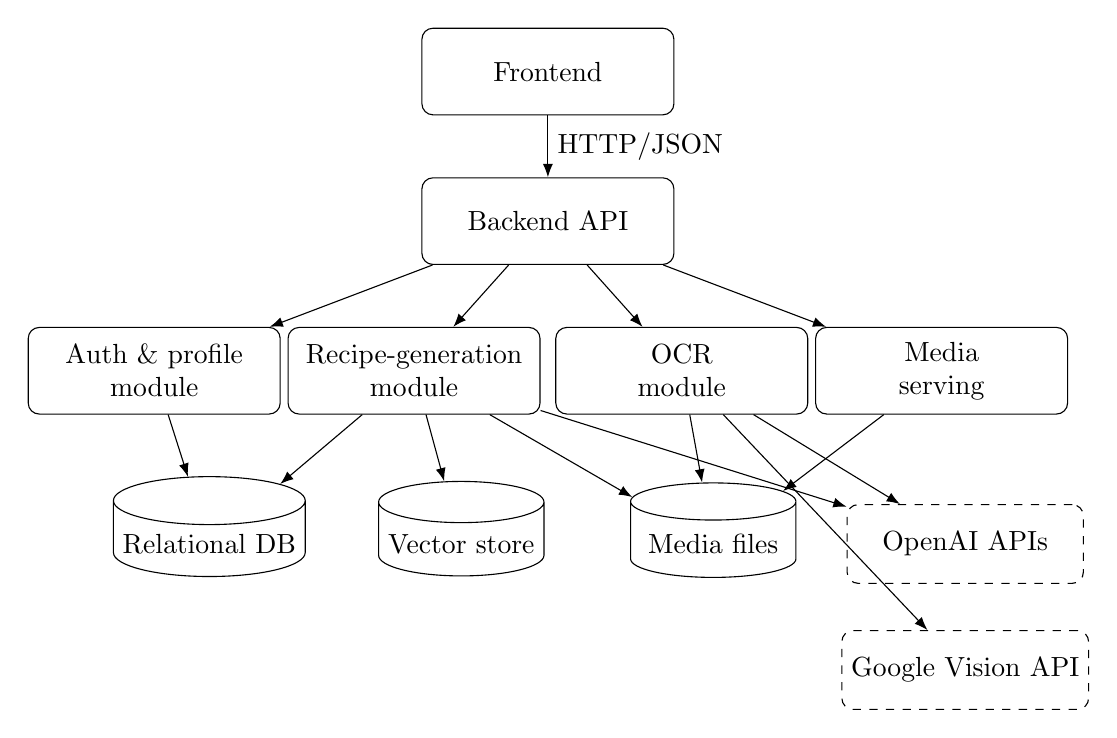
\begin{tikzpicture}[
		comp/.style={draw, rounded corners, minimum width=3.2cm, minimum height=1.1cm, align=center},
		store/.style={draw, cylinder, shape border rotate=90, aspect=0.25, minimum height=1.2cm, minimum width=2.1cm, align=center},
		ext/.style={draw, rounded corners, dashed, minimum width=3.0cm, minimum height=1.0cm, align=center},
		>=Latex
	]
	\node[comp] (frontend) at (0,5.6) {Frontend};
	\node[comp] (backend) at (0,3.7) {Backend API};

	\node[comp] (auth) at (-5.0,1.8) {Auth \& profile\\module};
	\node[comp] (recipes) at (-1.7,1.8) {Recipe-generation\\module};
	\node[comp] (ocr) at (1.7,1.8) {OCR\\module};
	\node[comp] (media) at (5.0,1.8) {Media\\serving};

	\node[store] (db) at (-4.3,-0.4) {Relational DB};
	\node[store] (chroma) at (-1.1,-0.4) {Vector store};
	\node[store] (files) at (2.1,-0.4) {Media files};
	\node[ext] (openai) at (5.3,-0.4) {OpenAI APIs};
	\node[ext] (vision) at (5.3,-2.0) {Google Vision API};

	\draw[-Latex] (frontend) -- node[right] {HTTP/JSON} (backend);

	\draw[-Latex] (backend) -- (auth);
	\draw[-Latex] (backend) -- (recipes);
	\draw[-Latex] (backend) -- (ocr);
	\draw[-Latex] (backend) -- (media);

	\draw[-Latex] (auth) -- (db);
	\draw[-Latex] (recipes) -- (db);
	\draw[-Latex] (recipes) -- (chroma);
	\draw[-Latex] (recipes) -- (files);
	\draw[-Latex] (recipes) -- (openai);
	\draw[-Latex] (ocr) -- (files);
	\draw[-Latex] (ocr) -- (vision);
	\draw[-Latex] (ocr) -- (openai);
	\draw[-Latex] (media) -- (files);
	\end{tikzpicture}}
	\caption{Component diagram of the system architecture}
	\label{fig:design-component}
\end{figure}

The component model also makes the layer boundaries visible. The
frontend never accesses the relational database, vector store, or
provider APIs directly. It talks only to the backend API. Within the backend, route modules remain
thin and delegate non-trivial work to services, providers, and storage
abstractions. This same decomposition reappears in the more detailed UML
artifacts presented next.

\begin{table}[H]
	\centering
	\scriptsize
	\renewcommand{\arraystretch}{1.2}
	\begin{tabularx}{\textwidth}{|p{2.8cm}|p{4.4cm}|X|}
		\hline
		\textbf{Layer} & \textbf{Implemented units} & \textbf{Primary responsibility} \\
		\hline
		Frontend interaction layer & React pages, navigation shell, shared auth context, reusable presentation components & Collect user input, maintain page-level interaction state, invoke backend routes, and render generated or retrieved results. \\
		\hline
		API boundary & FastAPI route modules and Pydantic request/response schemas & Validate request shape, enforce authentication or ownership checks, and expose a stable JSON contract to the browser. \\
		\hline
		Workflow and orchestration layer & Recipe-generation, OCR, retrieval, and image services & Execute multi-step application logic in a fixed order and isolate external-provider interactions from route handlers. \\
		\hline
		Provider integration layer & OCR and image-provider abstractions plus concrete adapters & Hide vendor-specific SDK calls behind application-facing interfaces such as \texttt{extract\_text()} and \texttt{generate\_png()}. \\
		\hline
		Transactional persistence layer & SQLAlchemy entities, database session handling, Alembic migrations & Store user accounts, generated recipes, OCR history, ownership relations, and pagination-supporting indexes. \\
		\hline
		Retrieval and media layer & Chroma vector store, recipe-indexing scripts, filesystem media storage & Persist retrieval documents and embeddings, store OCR uploads and thumbnails, and serve media files back to the frontend. \\
		\hline
	\end{tabularx}
\caption{Layer responsibilities in the implemented system}
	\label{tab:layer-responsibilities}
\end{table}

\subsubsection{Technology selection rationale}

The selected technologies follow the needs of the implemented
architecture instead of being chosen as a generic full-stack template.
The frontend is built as a React single-page application because the
main user tasks---recipe generation, OCR extraction, saved results, and
history browsing---share one navigation shell but require different
forms, loading states, and result layouts. A page-oriented React
frontend keeps those task flows separate while still allowing shared
authentication state and reusable result components.

The backend is built with FastAPI because the application depends on
clear request validation and on keeping route handlers thin. Recipe
generation, OCR extraction, save operations, and history listing all
accept structured input and return structured output, so schema-based
request and response handling fits the project well. This is especially
useful in the recipe workflow, where ingredient lists, allergies,
preferences, warnings, and nutrition fields all have to remain
well-formed across several processing stages.

Relational persistence is handled through SQLAlchemy with migration
support, because the project stores ownership-sensitive data rather than
anonymous prompt logs. User accounts, generated recipes, save state, and
OCR history need stable identifiers, foreign-key relationships, and
queryable timestamps. These requirements match a relational model more
closely than a document-only store.

The retrieval layer uses a persistent vector store because recipe
generation is grounded in a local recipe corpus. The system does not use
retrieval as an optional enhancement; it depends on retrieval to supply
context before prompt construction. For that reason, embeddings and
similarity search are treated as part of the architecture itself.

Media files are stored on the local filesystem because OCR uploads and
generated thumbnails act as supporting assets around the main
application data. The project needs these files to be saved, reused, and
served back to the frontend, but it does not need cloud-scale media
infrastructure for the bachelor-thesis scope. External AI providers are
used only where the project needs capabilities that are not implemented
locally, namely text generation, embeddings, OCR, and thumbnail
generation.

\subsubsection{Object-oriented modelling artifacts}

Although part of the backend is implemented in a function-oriented
style, the system still has a meaningful object-oriented structure. The
most important implemented classes fall into three groups:

\begin{itemize}
	\item \textbf{Persistent domain classes}, such as \texttt{User},
	\texttt{GeneratedRecipe}, and \texttt{OcrExtraction}.
	\item \textbf{Schema/data-transfer classes}, such as request and
	response models used at API boundaries.
	\item \textbf{Provider abstraction classes}, such as
	\texttt{OcrProvider}, \texttt{GoogleVisionOcrProvider},
	\texttt{RecipeImageProvider}, and
	\texttt{OpenAIRecipeImageProvider}.
\end{itemize}

The following class diagrams expand the earlier component view into the
implemented backend structures. The overview is split into two figures
to keep the diagrams readable at thesis page scale: one diagram focuses
on domain classes, provider abstractions, and the module-level service
boundaries around them, while the other focuses on schemas,
configuration, and infrastructure support.

\begin{figure}[htbp]
	\centering
	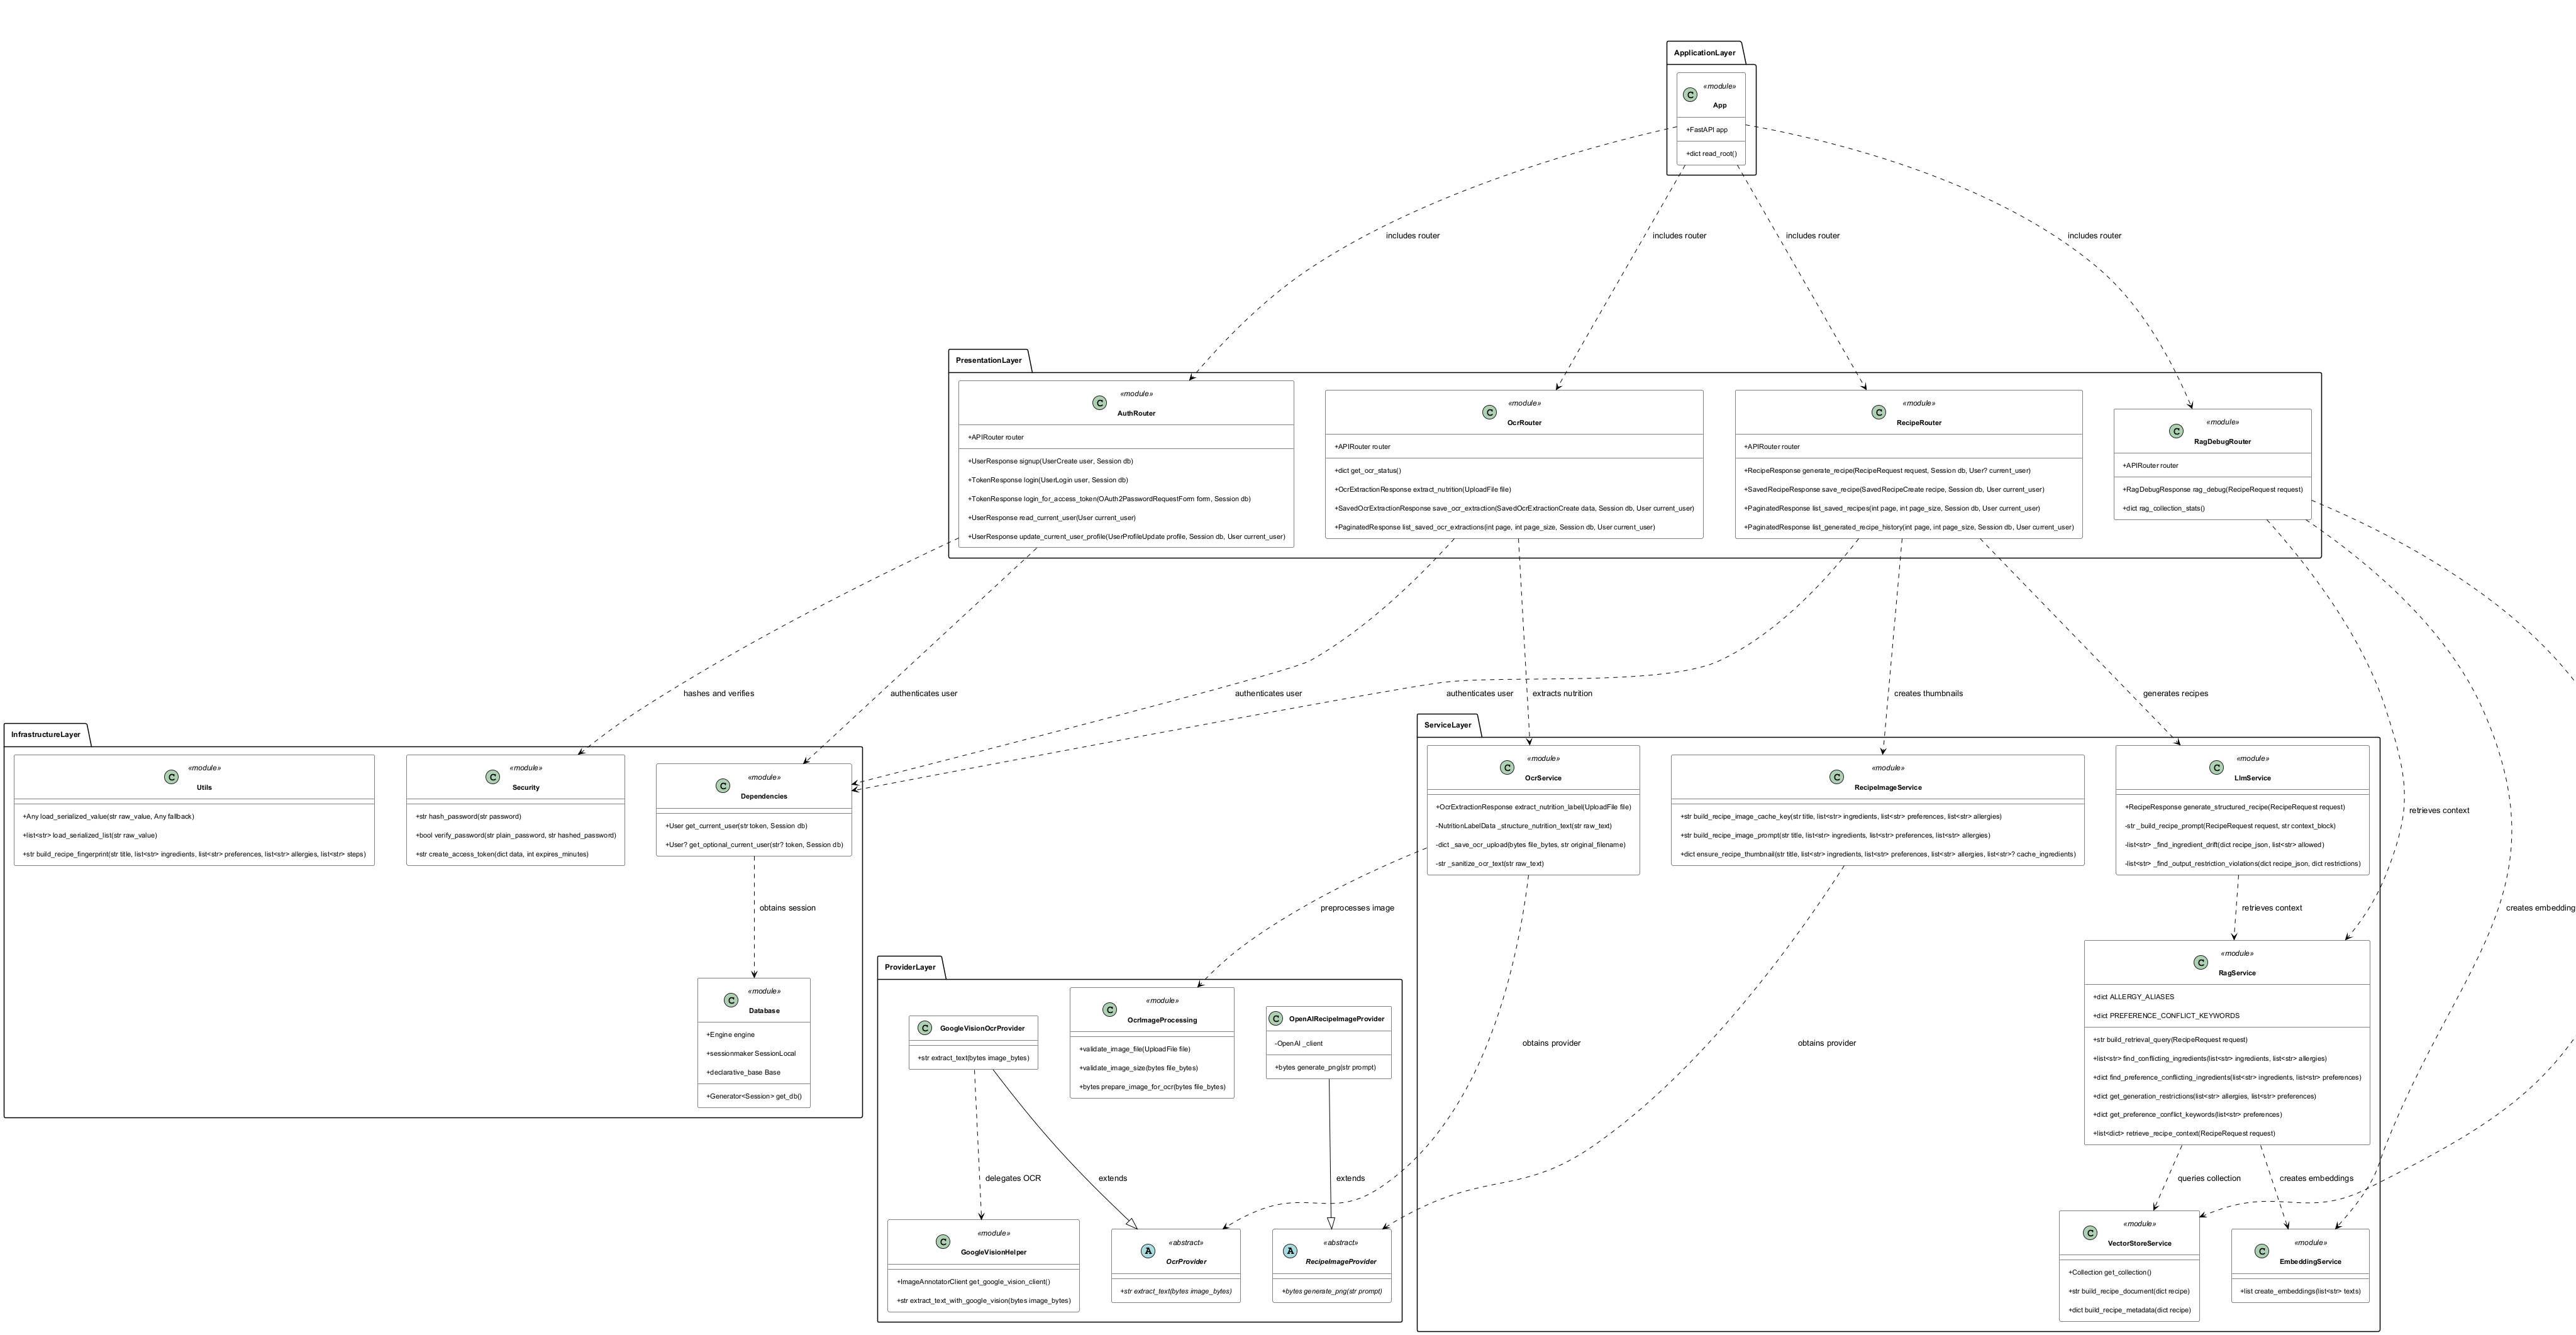
\includegraphics[width=\textwidth]{images/class-diagram-a.png}
	\caption{Class diagram of the domain and backend-service
	structure, showing implemented entity classes, provider
	abstractions, and their relationships}
	\label{fig:class-domain}
\end{figure}

\begin{figure}[htbp]
	\centering
	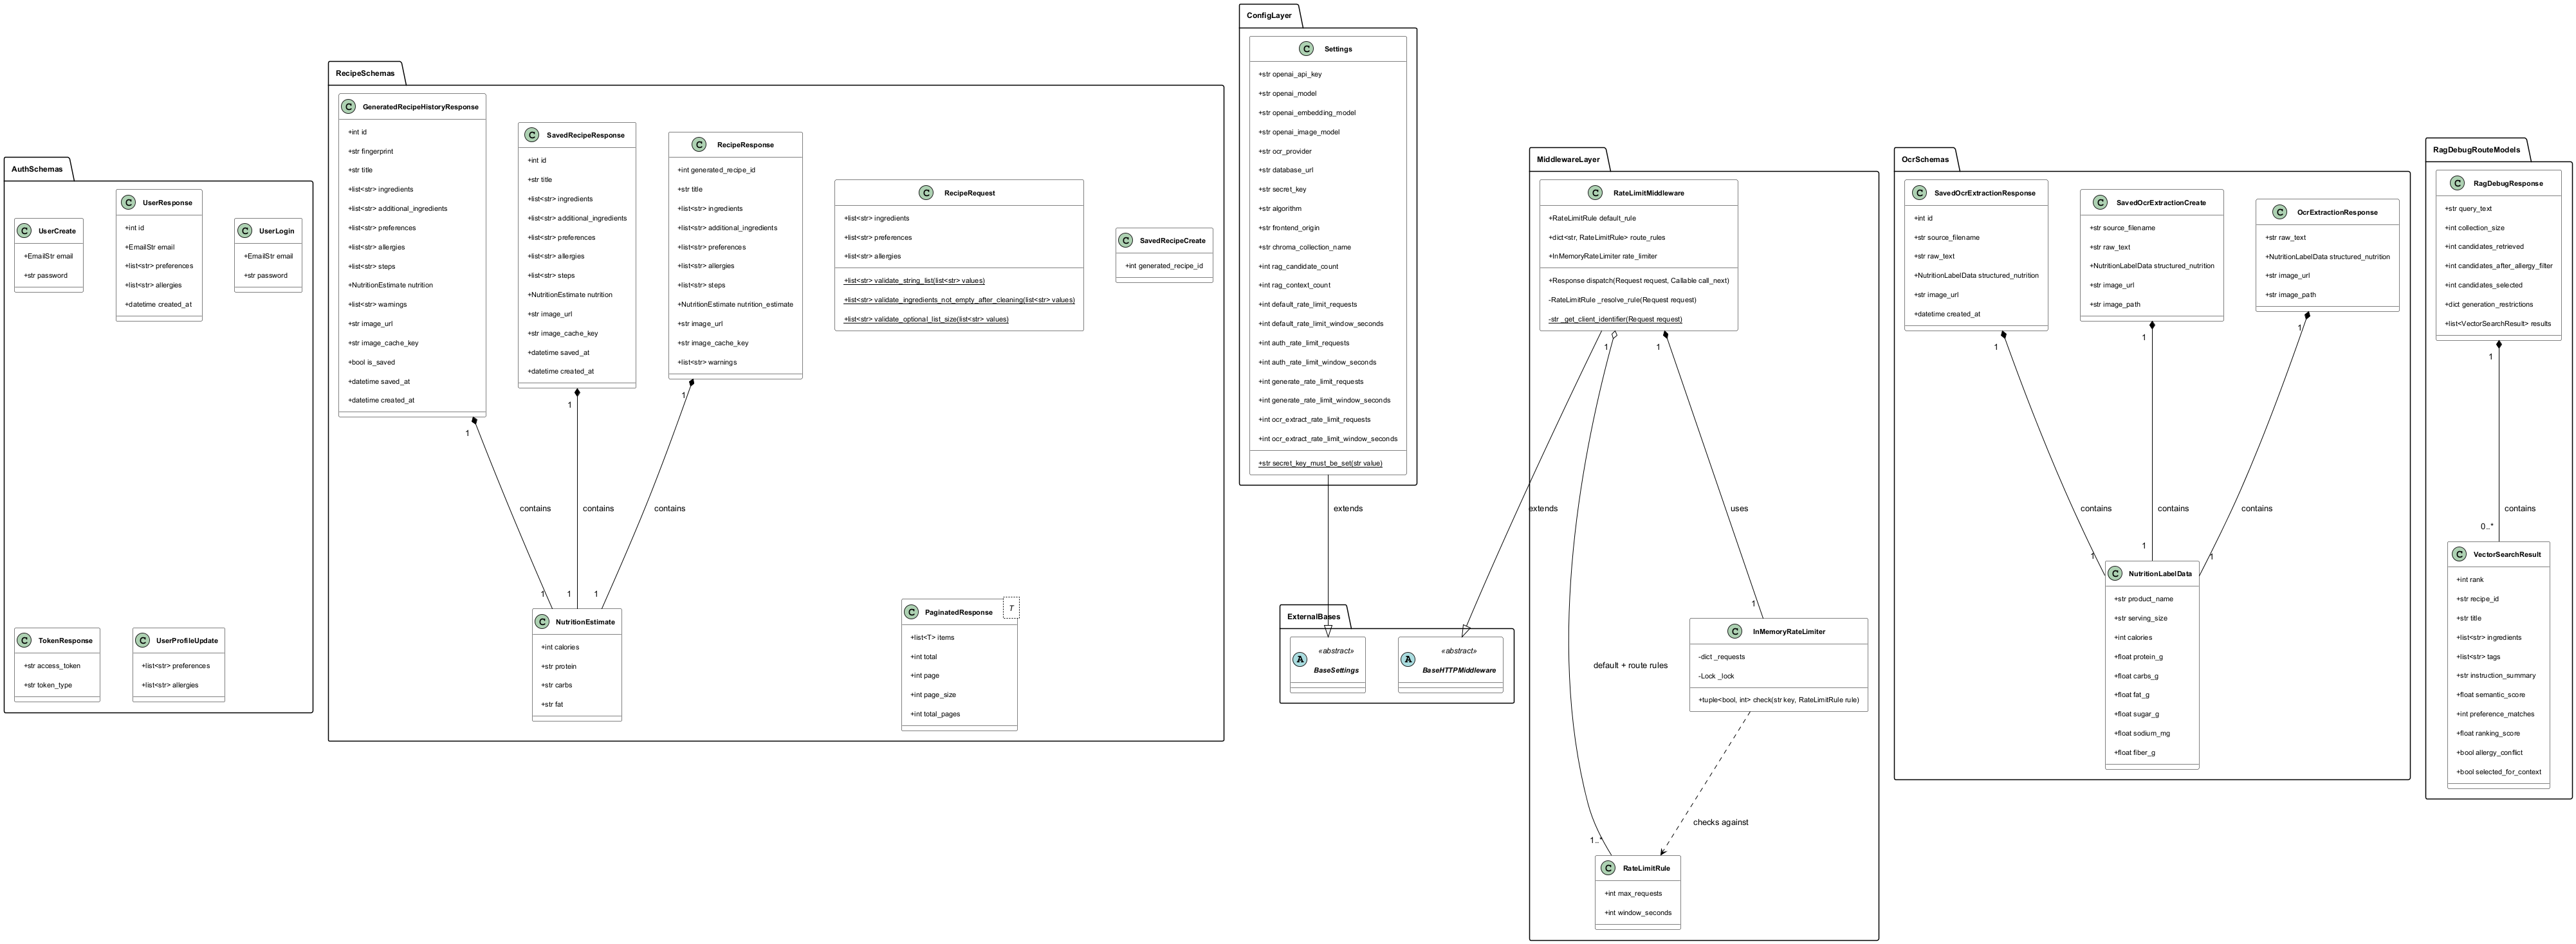
\includegraphics[width=\textwidth]{images/class-diagram-b.png}
	\caption{Class diagram of the infrastructure and schema
	layer, showing API contracts, configuration, middleware,
	and rate-limiting components}
	\label{fig:class-infrastructure}
\end{figure}

These diagrams describe the implemented structure of the system. The
persistent entities correspond to the relational model, the schema
classes define the API boundary, and the provider abstractions separate
vendor-specific OCR and image-generation logic from the rest of the
application. They are mixed on purpose: some parts of the backend are
class-based, while others are clearer as service modules. The diagrams
follow that split instead of pretending that every part of the system
fits one style equally well.

To make this correspondence explicit, Table~\ref{tab:diagram-code-map}
links the main structural artifacts to the implementation units they
describe most directly.

\begin{table}[H]
	\centering
	\scriptsize
	\renewcommand{\arraystretch}{1.2}
	\begin{tabularx}{\textwidth}{|p{2.8cm}|p{4.8cm}|X|}
		\hline
		\textbf{Diagram artifact} & \textbf{Most visible implemented elements} & \textbf{Implementation area} \\
		\hline
		Domain/service class view & \texttt{User}, \texttt{GeneratedRecipe}, \texttt{OcrExtraction}, provider abstractions, route-to-service dependencies & Domain model, recipe workflow services, OCR workflow services, and provider abstractions. \\
		\hline
		Infrastructure/schema class view & \texttt{Settings}, \texttt{RateLimitMiddleware}, \texttt{RateLimitRule}, request and response schemas & Configuration, middleware, and schema-definition modules. \\
		\hline
		Sequence view of recipe generation & Route entry, generation service, retrieval service, provider calls, conditional persistence & Recipe route handling together with retrieval and generation services. \\
		\hline
		State-transition view & Validation, filtering, retrieval, retry, image generation, authenticated persistence & Request validation, recipe orchestration, and thumbnail-generation modules. \\
		\hline
		Use-case and navigation views & User-visible routes and persistence-related page separation & Frontend routing, task pages, and authenticated navigation views. \\
		\hline
		ER and relational views & Entity ownership, nullable vs non-null foreign keys, indexes, and denormalized payload fields & ORM entity definitions and schema-migration history. \\
		\hline
	\end{tabularx}
	\caption{Direct correspondence between the design artifacts and the implementation units}
	\label{tab:diagram-code-map}
\end{table}

\subsubsection{Core workflow design}

The most important backend behavior is not a static entity relation but
a controlled multi-stage workflow. Recipe generation especially benefits
from dynamic modelling because its correctness depends on the order of
operations: validation must happen before retrieval, retrieval before
prompt construction, and output checking before persistence.

The following sequence diagram captures the expected interaction path
for a recipe request. It shows how the frontend, backend route, service
layer, retrieval subsystem, and provider calls cooperate during a single
end-to-end generation.

\begin{figure}[p]
	\centering
	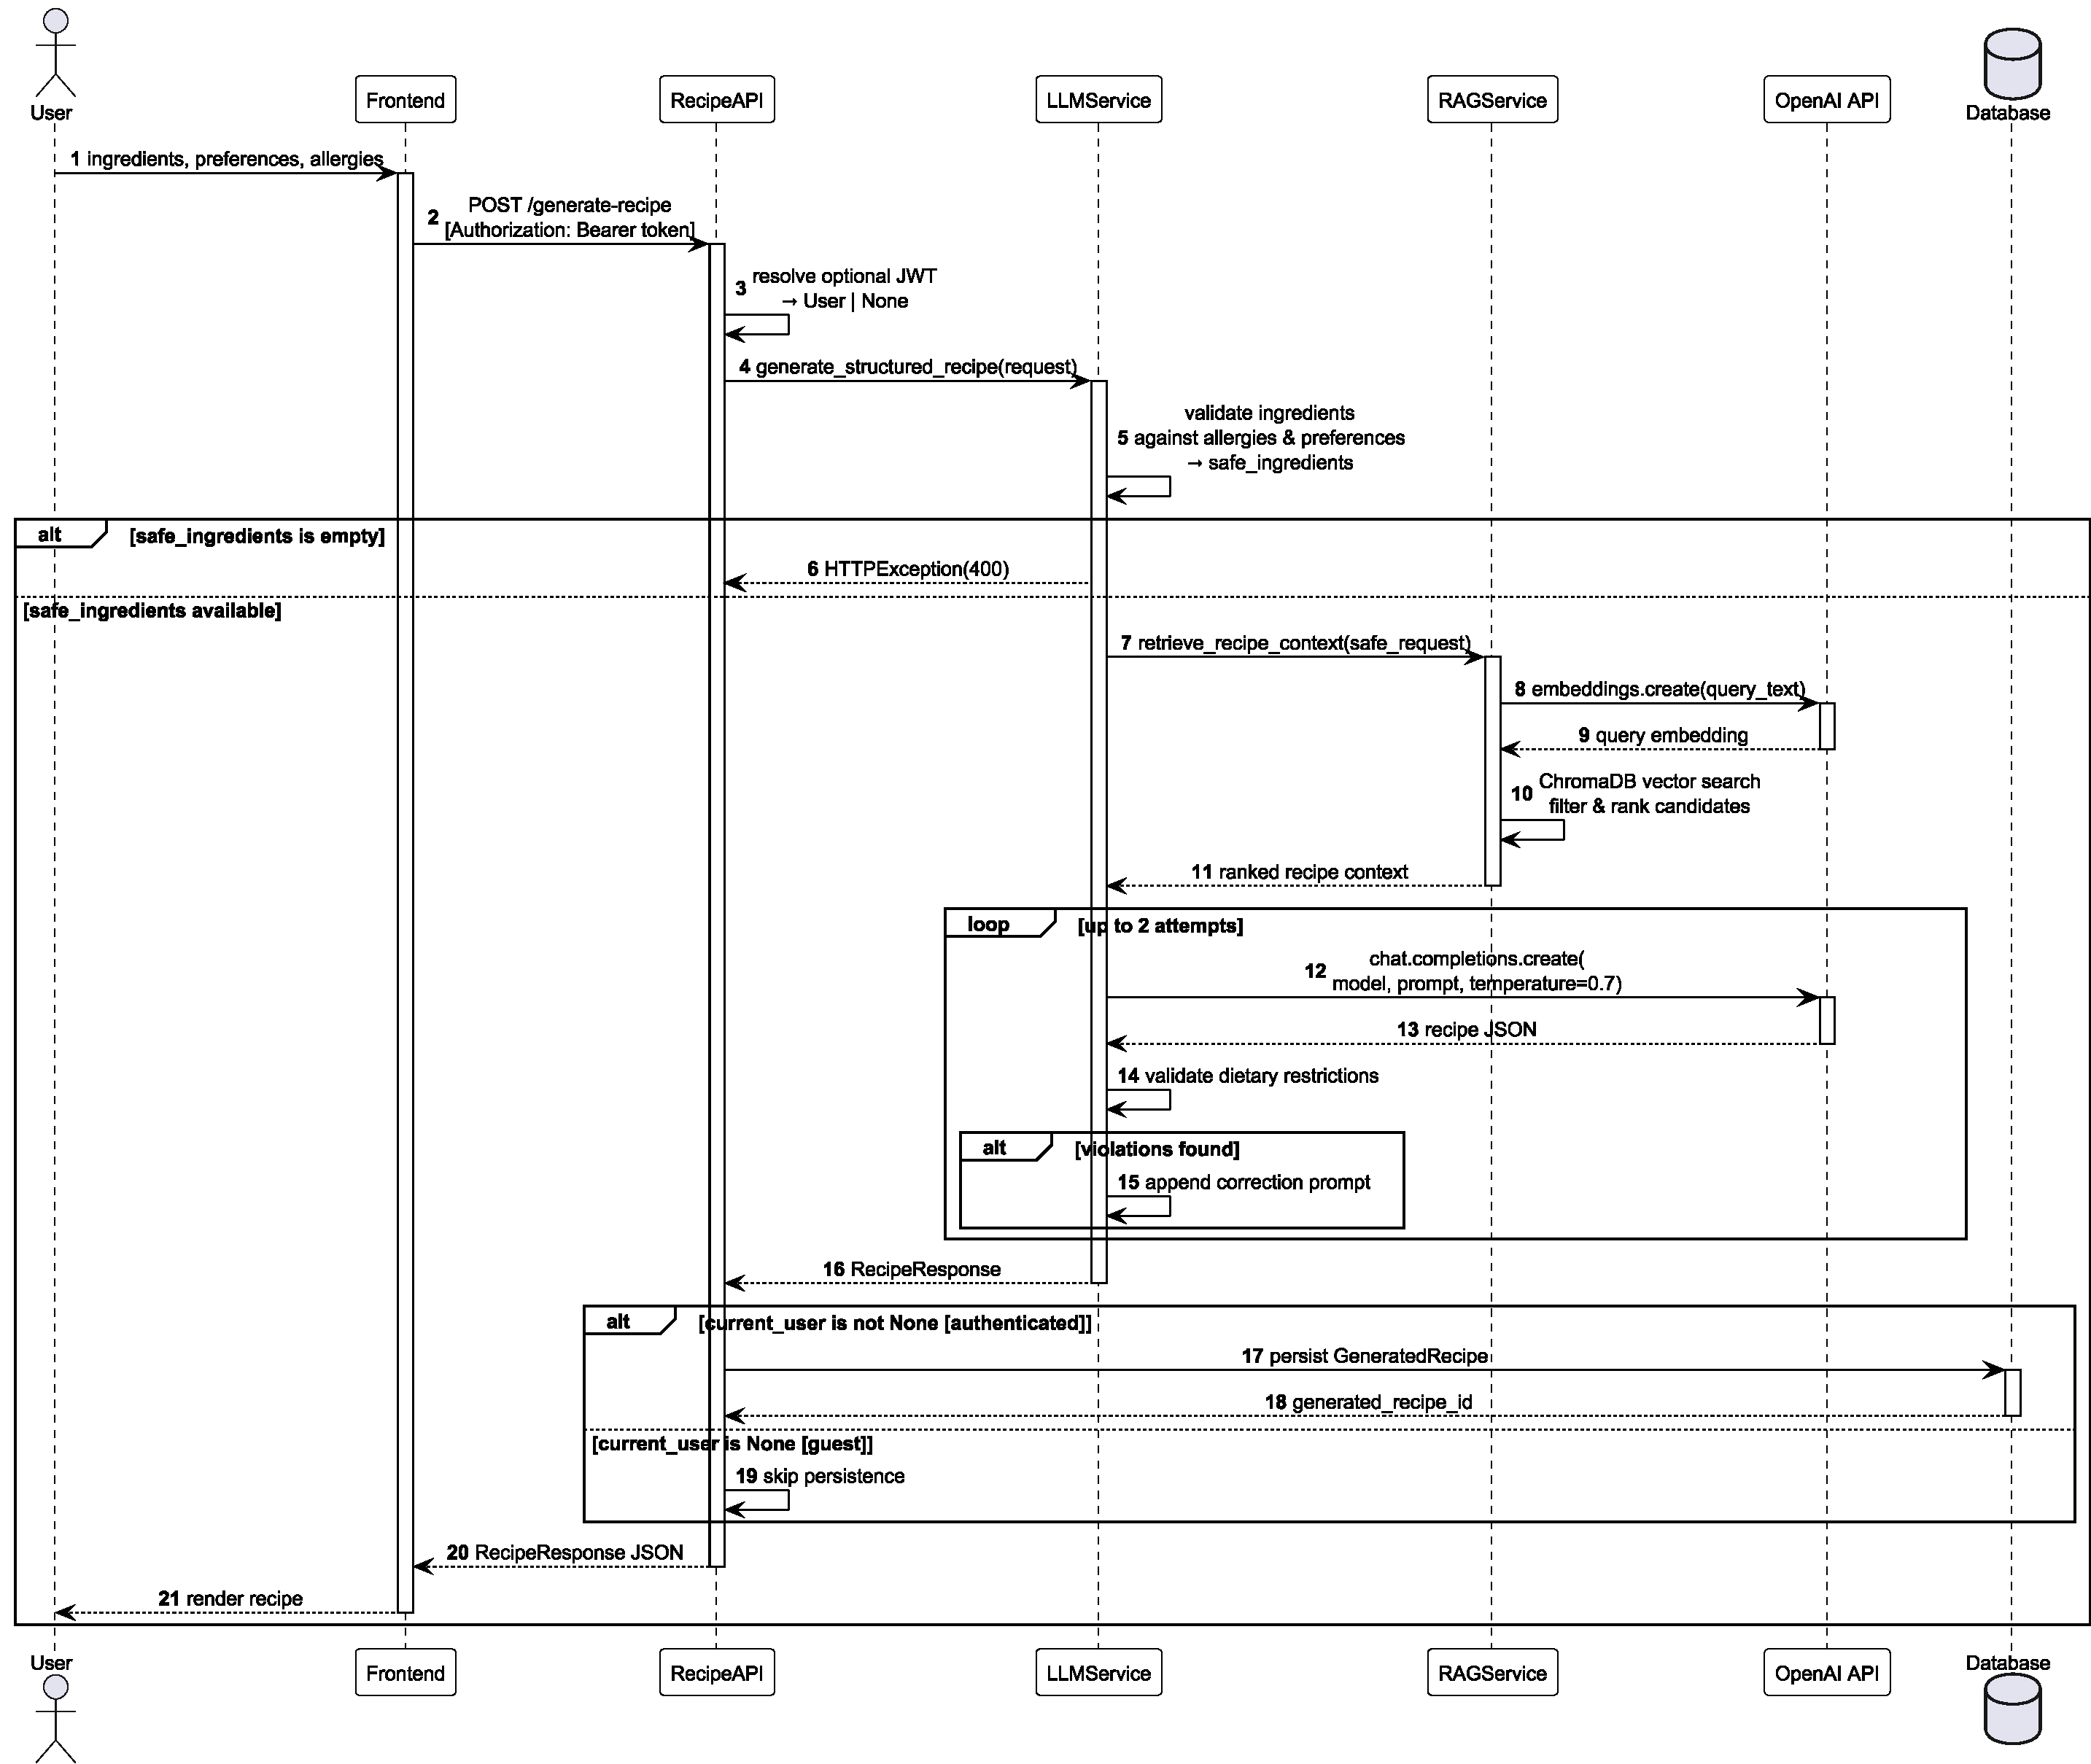
\includegraphics[width=\textwidth]{images/sequence-recipe-generation.pdf}
	\caption{Sequence diagram of the recipe-generation workflow,
	illustrating the call chain from user input through context retrieval,
	LLM invocation, and conditional database persistence}
	\label{fig:design-sequence}
\end{figure}

The sequence view is complemented by a state-oriented and a data-flow
view. The state machine is useful because a recipe request may pass
through correction states before it becomes acceptable, and because
thumbnail generation is intentionally modelled as a non-fatal step. The
data flow diagram is useful because it clarifies which data is produced
or transformed at each stage and which stores participate in the
pipeline. Together, these views document the static structure and the
dynamic behavior of the system from complementary angles.

\begin{figure}[p]
	\centering
	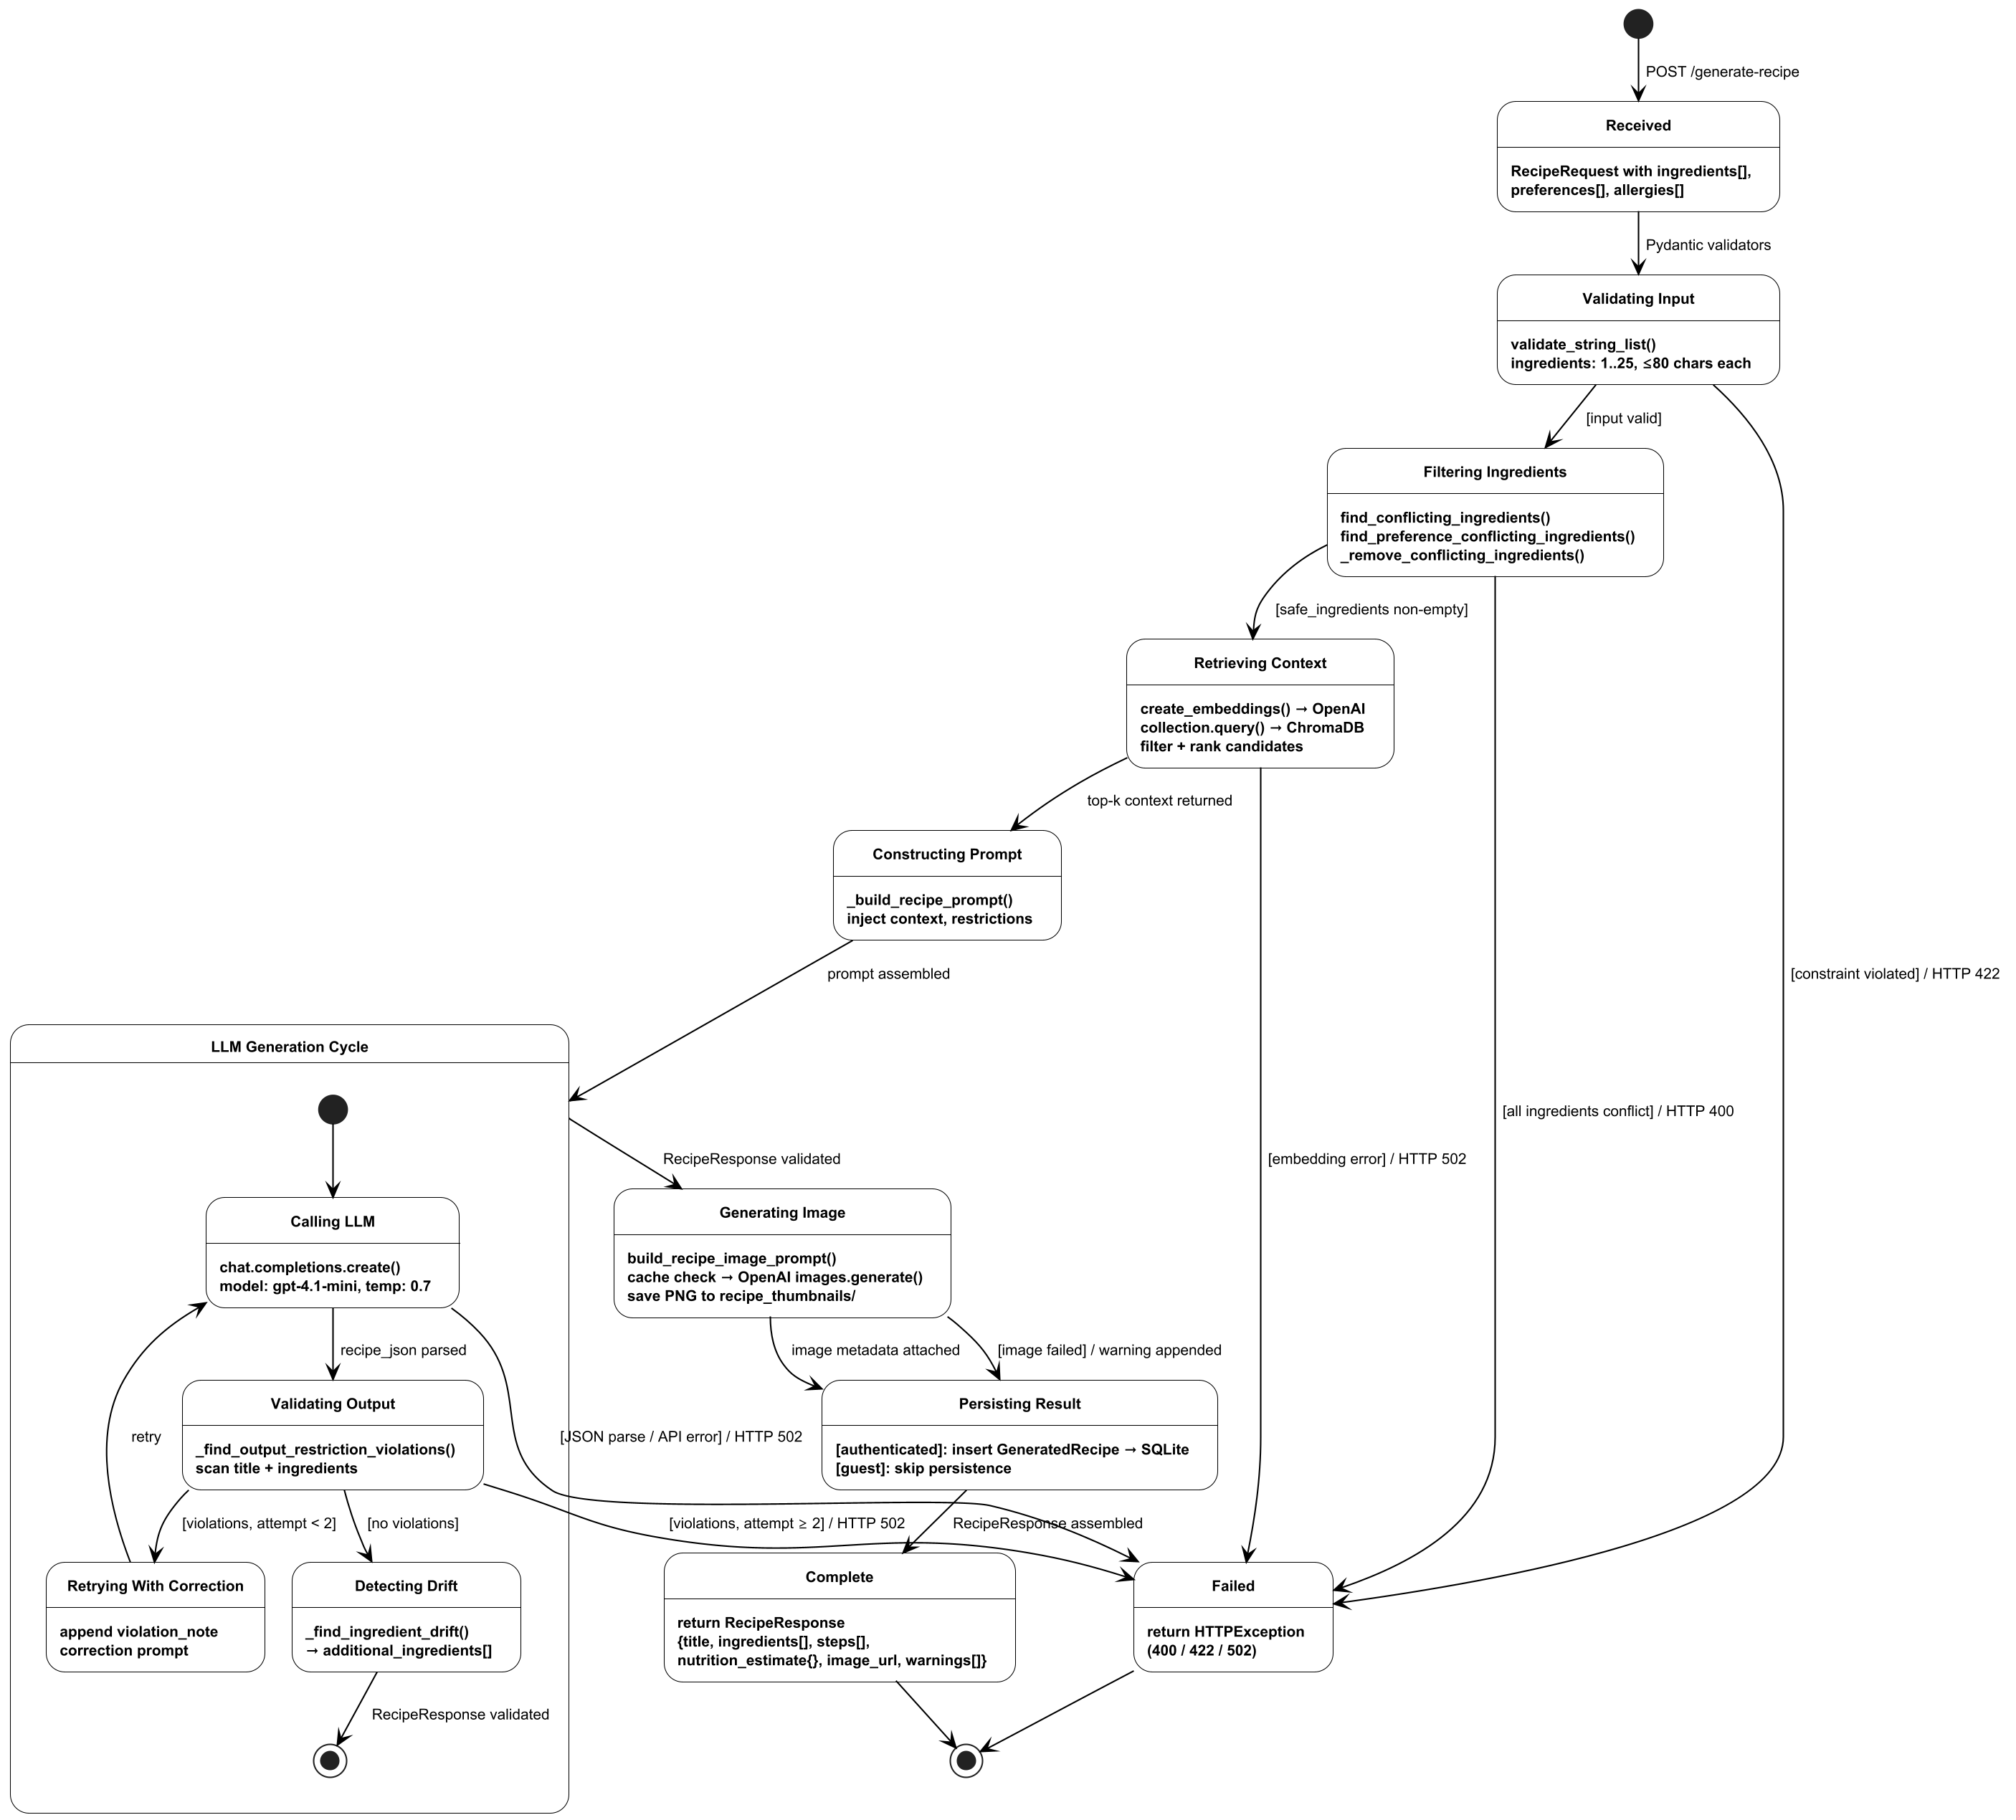
\includegraphics[width=\textwidth,height=0.85\textheight,keepaspectratio]{images/state-transition-recipe-lifecycle.png}
	\caption{State-transition diagram of the recipe request lifecycle,
	showing the path from initial submission through input validation,
	ingredient filtering, retrieval-augmented generation, output
	verification, thumbnail generation, and persistence}
	\label{fig:state-transition}
\end{figure}

\begin{figure}[p]
	\centering
	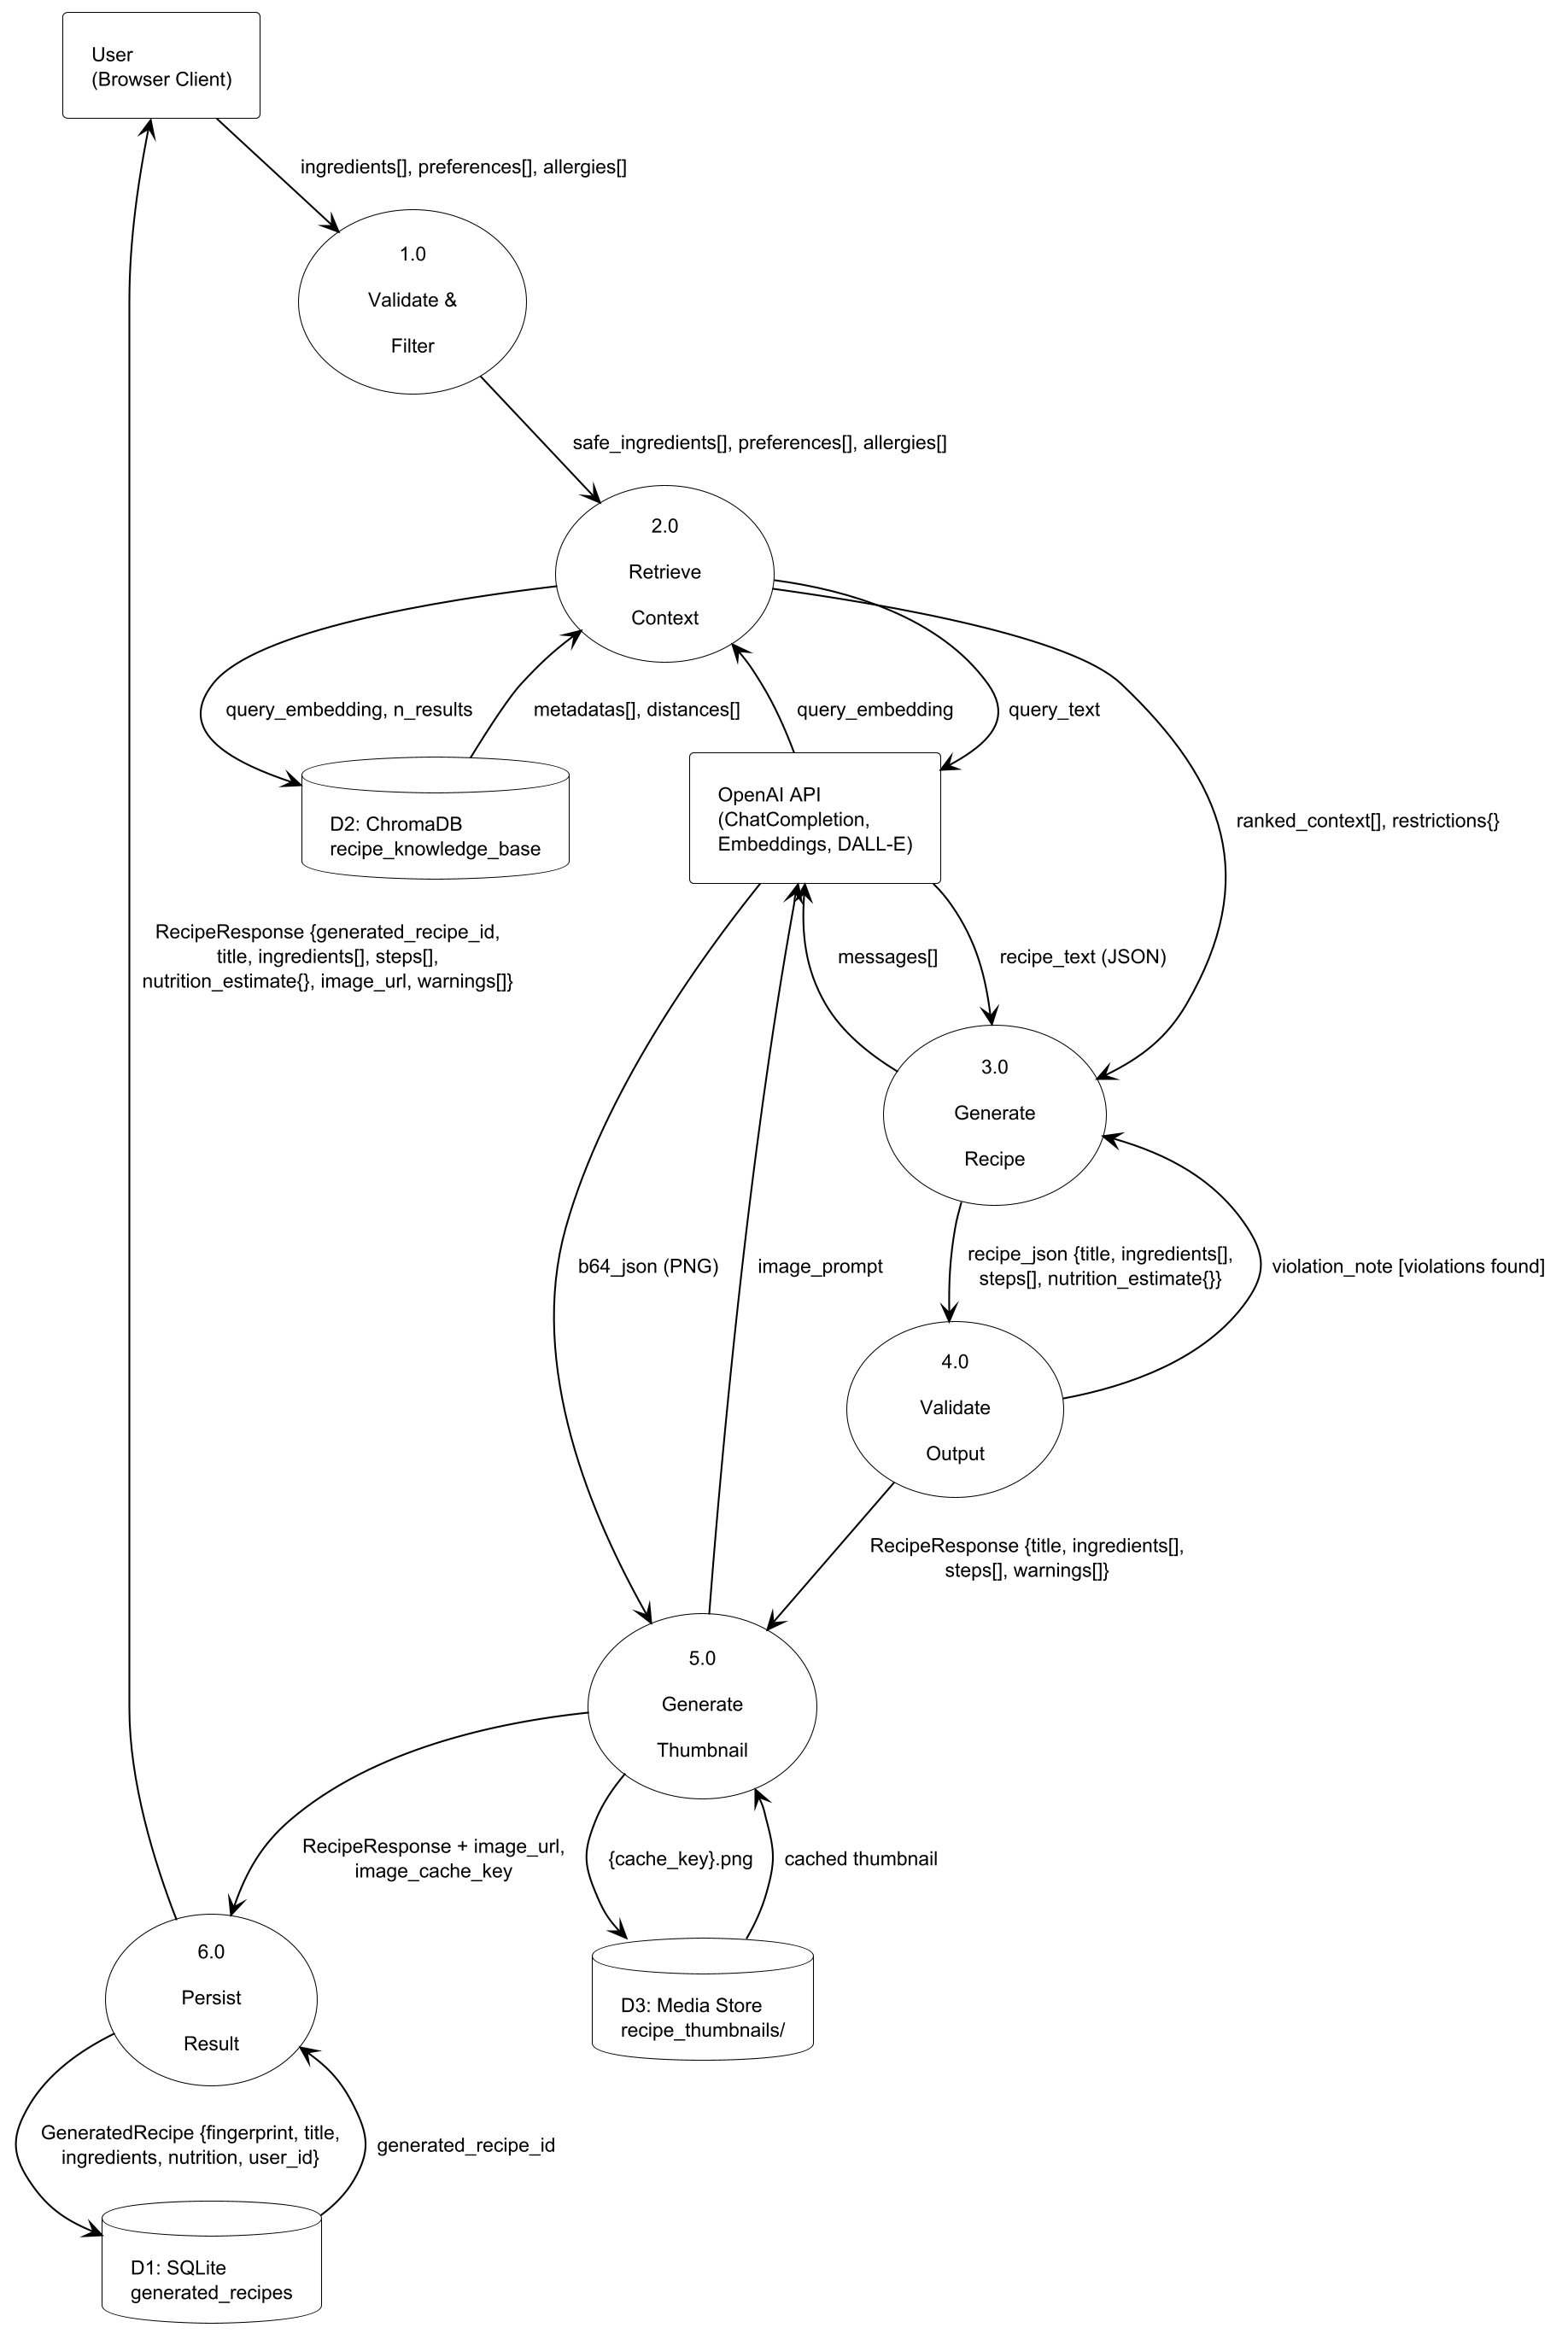
\includegraphics[width=\textwidth,height=0.85\textheight,keepaspectratio]{images/dfd-recipe-generation.png}
	\caption{Level~1 data flow diagram of the recipe-generation
	pipeline, showing processes, data stores, external entities, and
	field-level flows derived from the application codebase}
	\label{fig:dfd}
\end{figure}

Two design decisions are especially important at workflow level.
First, recipe generation is not a single prompt call. The workflow
performs input cleaning, conflict detection, safe-context retrieval,
prompt construction, output validation, optional retry, optional image
generation, and conditional persistence. Second, OCR is explicitly split
into optical extraction and semantic structuring. This separation keeps
failure causes easier to diagnose and allows the OCR provider and the
nutrition-structuring logic to evolve independently.

\subsubsection{API design and interaction model}

The frontend communicates with the backend almost entirely through JSON
API requests. The only exception is OCR upload, where the image itself
is transferred as multipart form data before the backend returns a
structured JSON result. In all cases, the interaction model remains the
same: the frontend sends user input to a dedicated backend route, the
backend validates the request, executes the relevant workflow, and
returns a structured response that the frontend can render directly.

This interaction model keeps the frontend simple. Each page only needs
to know which route to call and what response structure to expect. The
backend remains responsible for authentication, ownership checks,
workflow order, provider calls, and persistence.

\begin{table}[H]
	\centering
	\scriptsize
	\begin{tabular}{|p{2.8cm}|p{11.1cm}|}
		\hline
		\textbf{API area} & \textbf{Purpose and example responsibilities} \\
		\hline
		Authentication API & Supports signup, login, token issuance, current-user retrieval, and profile-default updates. Protected profile operations require authentication and always operate on the resolved current user rather than on client-supplied ownership identifiers. \\
		\hline
		Recipe API & Accepts recipe-generation requests, returns structured recipes with warnings and optional image metadata, persists generated history for authenticated users, and exposes saved-recipe and full-history listings filtered by the authenticated owner. \\
		\hline
		OCR API & Accepts nutrition-label uploads, validates image payloads, returns raw OCR text together with structured nutrition fields, and allows authenticated users to save and browse OCR history under their own account scope. \\
		\hline
		Media/static API & Exposes backend-managed OCR uploads and generated thumbnails as static files addressable from frontend result views and history pages. \\
		\hline
	\end{tabular}
	\caption{Main API areas and their responsibilities}
	\label{tab:api-areas}
\end{table}

\subsubsection{Decision transparency and user-visible evidence}

Because the application relies on external AI services, the design does
not hide intermediate evidence or corrective decisions from the user.
Transparency appears in several concrete forms. Recipe generation can
return warning messages when some provided ingredients were excluded,
when the generated result requires additional ingredients, or when
thumbnail generation fails and the recipe is returned without an image.
The OCR workflow displays the raw extracted text and the structured
nutrition interpretation side by side, which allows the user to judge
whether the semantic structuring step remained faithful to the visible
label content.

This transparency is part of making the system usable. OCR and
language-model services can still return imperfect results, so the
application should show what was read directly from the input and what
was inferred later in the workflow.

\subsubsection{Recurring design mechanisms}

The project uses a layered architecture together with a small number of
recurring design mechanisms that appear across multiple modules. This is
a better description of the system than forcing every decision into a
formal pattern taxonomy. The most important structural pressures in the
project are provider substitution, explicit API contracts, workflow
orchestration, and controlled persistence boundaries.

\begin{table}[H]
	\centering
	\scriptsize
	\renewcommand{\arraystretch}{1.2}
	\begin{tabularx}{\textwidth}{|p{2.5cm}|p{3.8cm}|p{3.8cm}|X|}
		\hline
		\textbf{Mechanism} & \textbf{Implemented form} & \textbf{Implementation area} & \textbf{Why it fits the system} \\
		\hline
		Provider substitution & OCR and image-generation interfaces with concrete implementations & Provider abstractions for OCR and recipe-image generation. & External providers can change without forcing route or workflow logic to depend on vendor-specific SDK calls. \\
		\hline
		Centralized provider construction & Backend-owned provider selection and reuse points & Provider setup and service initialization logic. & Route handlers and service code ask for capabilities, not concrete classes, which keeps creation logic out of application flow. \\
		\hline
		SDK adaptation & Thin wrappers around OpenAI and Google Vision calls & Concrete provider adapter modules. & External APIs are translated into application-level operations such as text extraction and image generation. \\
		\hline
		Service orchestration boundary & Route modules delegate non-trivial workflows to narrow service entry points & Route modules and workflow-service modules. & Multi-stage workflows stay reusable and testable instead of being duplicated across endpoints. \\
		\hline
		Validated data contracts & Request and response schemas separated from ORM entities & API schema layer. & API contracts remain explicit, validated, and independent from persistence concerns. \\
		\hline
		Cross-cutting middleware & Shared rate-limiting and CORS configuration installed at bootstrap time & Application bootstrap and middleware configuration. & Concerns that apply to many routes are kept out of endpoint logic and enforced uniformly. \\
		\hline
	\end{tabularx}
	\caption{Recurring design mechanisms used throughout the system}
	\label{tab:design-patterns}
\end{table}

These decisions matter mainly for maintainability. Route handlers do not
need to know how provider authentication works or how OCR and image
payloads are encoded; they rely on service or provider interfaces.
Likewise, the frontend depends on API contracts instead of the database
schema. That separation is useful in this project because recipe
generation, OCR, retrieval, and persistence all meet in the same
application. Some parts are best described through classes and
relationships, while others are better described as step-by-step
workflows, and the design chapter follows that same split.

\subsection{Data Design}

\subsubsection{Storage responsibilities}

The system uses three forms of storage because the data has three
different roles:

\begin{itemize}
	\item \textbf{Relational storage} for users and historical user data.
	\item \textbf{Vector storage} for recipe-context retrieval.
	\item \textbf{Filesystem storage} for OCR upload images and generated
	thumbnails.
\end{itemize}

This storage split follows the way the application actually uses data.
User accounts and ownership relations fit a relational model. Retrieval
needs embeddings and similarity search. Uploaded images and thumbnails
are easiest to keep as files referenced from the application data.
The dynamic behavior around recipe generation is documented earlier
through the sequence, state-transition, and data-flow diagrams in
Section~3.2, because the non-trivial data transformations in this
project arise from workflow execution rather than from the static
relational model alone.

\subsubsection{Entity--relationship model}

The relational core of the system contains three entities:
\texttt{User}, \texttt{GeneratedRecipe}, and \texttt{OcrExtraction}.

\begin{itemize}
	\item A \texttt{User} stores identity and profile-default information.
	\item A \texttt{GeneratedRecipe} stores the result of a recipe
	generation request and whether the result was explicitly saved.
	\item An \texttt{OcrExtraction} stores the result of a nutrition-label
	extraction associated with a user.
\end{itemize}

The entity relationships are intentionally simple, because the main
complexity of the application lies in workflow logic rather than in a
large relational domain model:

\begin{itemize}
	\item one user may have many generated recipes,
	\item one user may have many OCR extractions,
	\item each generated recipe belongs to at most one user,
	\item each OCR extraction belongs to exactly one user.
\end{itemize}

\begin{figure}[H]
	\centering
	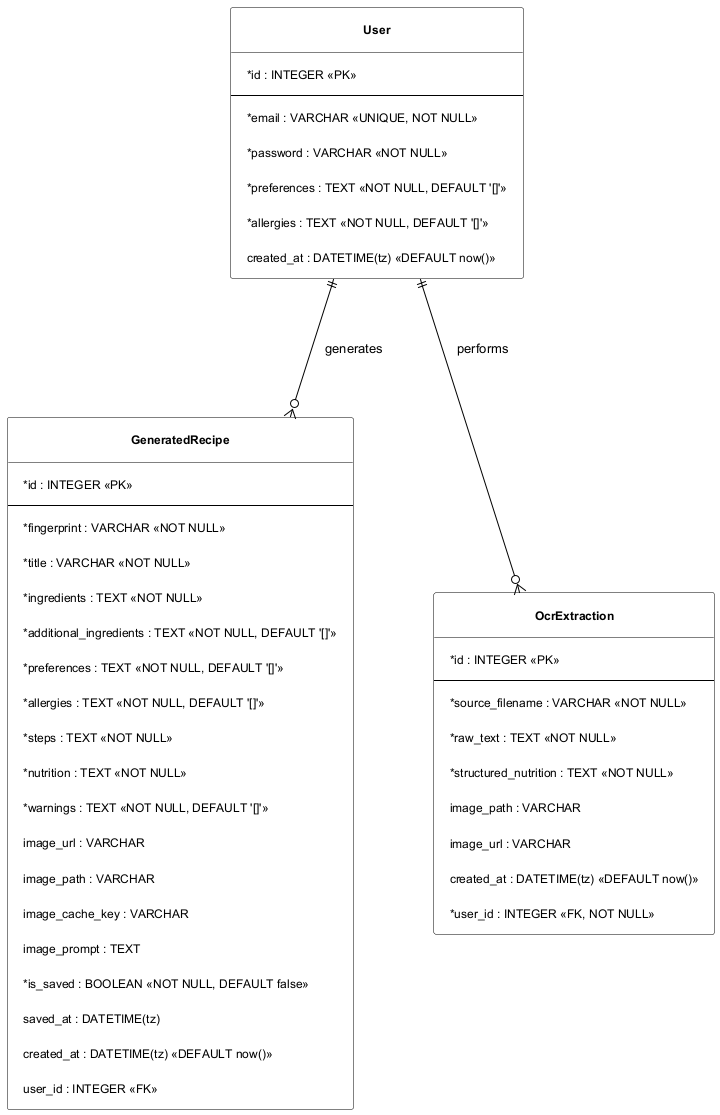
\includegraphics[width=\textwidth]{images/er-diagram.png}
	\caption{Entity-relationship diagram of the AI Cookbook system
	database, showing all entities, attributes, primary keys,
	foreign keys, and cardinality constraints}
	\label{fig:design-erd}
\end{figure}

\subsubsection{Derived relational schema}

From the ER model, the relational schema is derived as shown in
Figure~\ref{fig:relational-schema}. Every table is presented with its
complete column set, data types, key markers, integrity constraints, and
index definitions. The diagram makes the transformation from conceptual
entities to implementable tables explicit, which is important because
the application uses ORM classes but still relies on a concrete
relational design underneath.

The transformation from conceptual model to relational model is direct.
The \texttt{User} entity becomes the \texttt{users} table, the
\texttt{GeneratedRecipe} entity becomes the
\texttt{generated\_recipes} table, and the \texttt{OcrExtraction}
entity becomes the \texttt{ocr\_extractions} table. The two
one-to-many relationships from \texttt{User} are realized by the
\texttt{user\_id} foreign keys in \texttt{generated\_recipes} and
\texttt{ocr\_extractions}. In other words, the ER cardinality ``one
user may own many generated recipes'' is implemented as many rows in
\texttt{generated\_recipes} referencing one row in \texttt{users}, and
the same transformation is used for OCR history.

One detail deserves explicit mention. The
\texttt{generated\_recipes.user\_id} column is nullable at schema level.
This comes from the guest-generation flow, not from a different
ownership rule. The application allows guests to generate recipes, but
only authenticated users can persist them. Keeping the foreign key
nullable makes the schema compatible with that flow, while the
application logic still decides when persistence is allowed. By
contrast, \texttt{ocr\_extractions.user\_id} is non-null because OCR
history entries are created only through an authenticated save action.

\begin{figure}[H]
	\centering
	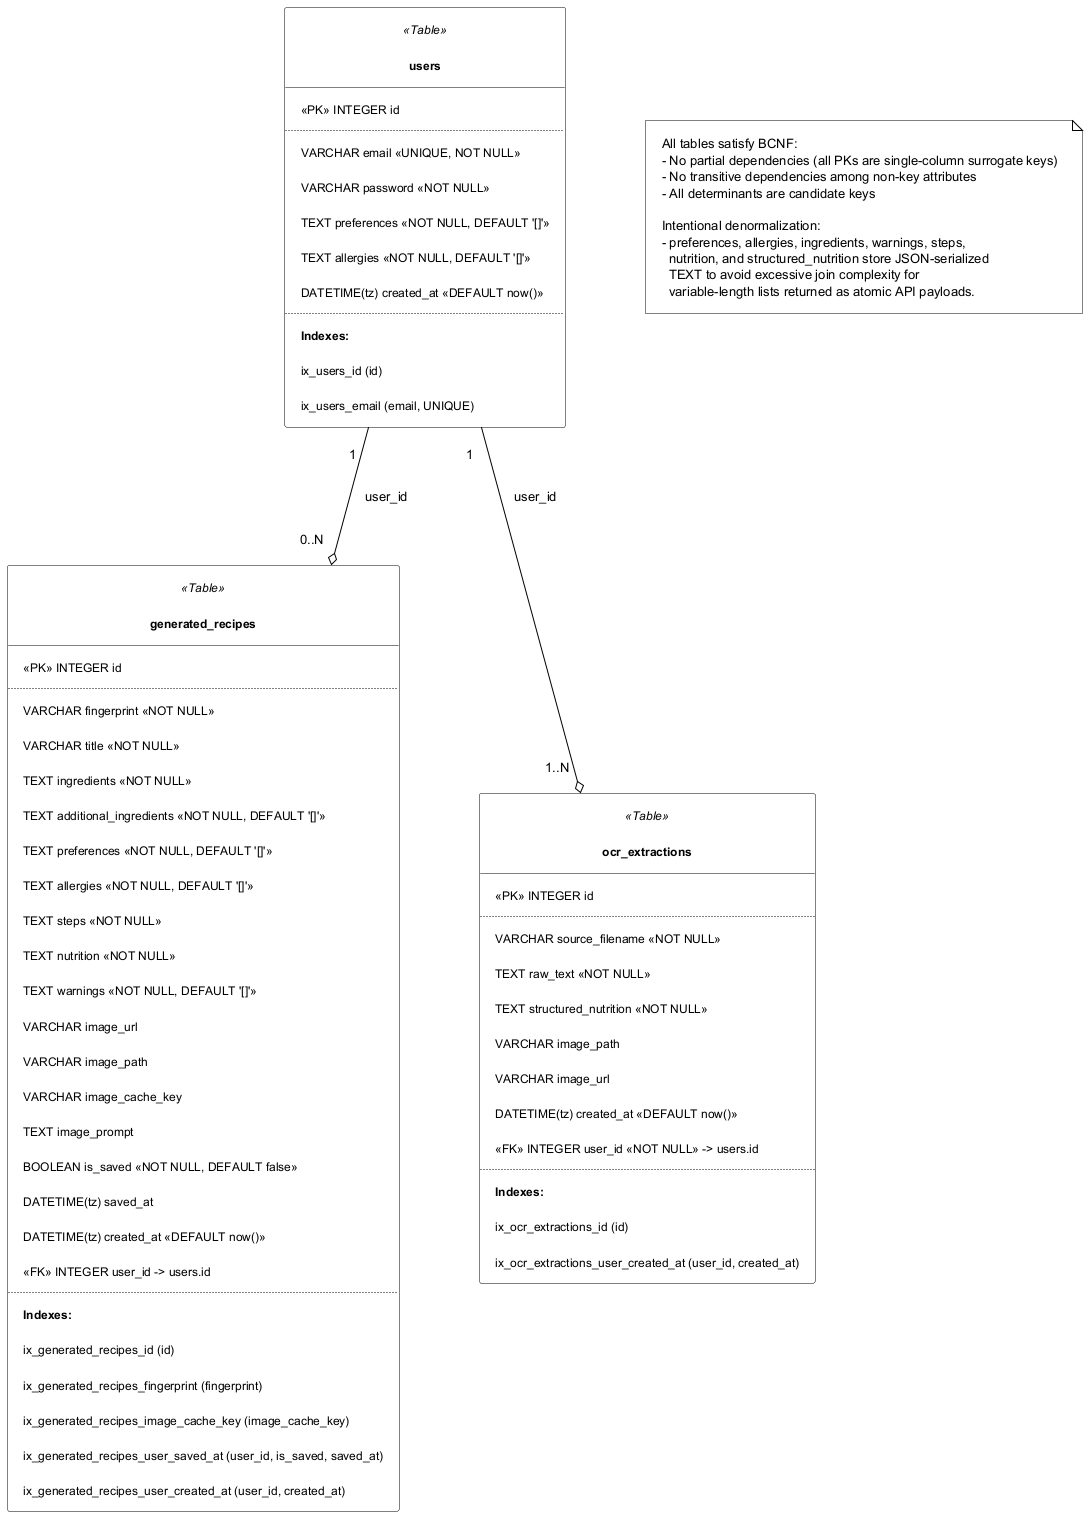
\includegraphics[width=\textwidth]{images/relational-schema.png}
	\caption{Relational schema derived from the ER model, showing all
	tables with primary keys, foreign keys, constraints, indexes, and
	inter-table relationships}
	\label{fig:relational-schema}
\end{figure}

\subsubsection{Normalization analysis}

The database schema of the AI Cookbook system consists of three
relations: \texttt{users}, \texttt{generated\_recipes}, and
\texttt{ocr\_extractions}. Each relation uses a single-column
surrogate integer primary key (\texttt{id}), which makes partial
dependencies structurally impossible and keeps ownership relations easy
to express through foreign keys.

At the relational level, the schema satisfies the usual normalization
requirements up to BCNF. The tables do not contain repeating groups,
their non-key attributes depend on the whole primary key, and there are
no transitive dependencies in which one non-key attribute determines
another. The strongest project-specific example is \texttt{users}: the
unique \texttt{email} attribute supports authentication lookup, while
\texttt{password}, \texttt{preferences}, \texttt{allergies}, and
\texttt{created\_at} all remain directly dependent on the row identity.
The same reasoning applies to \texttt{generated\_recipes} and
\texttt{ocr\_extractions}, where \texttt{user\_id} expresses ownership
but does not determine the remaining descriptive attributes of the row.

The schema does contain intentional denormalization in several
\texttt{TEXT} columns that store JSON-serialized arrays or objects
rather than being decomposed into separate child tables.
Specifically, the \texttt{preferences} and \texttt{allergies}
columns in both \texttt{users} and \texttt{generated\_recipes} store
serialized JSON arrays of strings. The \texttt{ingredients},
\texttt{additional\_ingredients}, \texttt{steps}, \texttt{warnings},
and \texttt{nutrition} columns in \texttt{generated\_recipes}, as
well as \texttt{structured\_nutrition} in
\texttt{ocr\_extractions}, similarly store JSON-encoded structured
data. A strictly normalized design would decompose each of these
into separate child relations. However, this denormalization is a
deliberate design choice driven by the application's access patterns:
every API endpoint that retrieves a recipe or extraction returns
these fields as complete JSON structures in a single response, and
the application never filters or aggregates on individual elements
within them at SQL level. Decomposing them would introduce extra join
cost and mapping complexity for every read while providing little
benefit to the actual queries used by the system.

\subsubsection{Index strategy and query design}

The index design reflects the dominant access paths of the application.

\begin{itemize}
	\item A unique index on \texttt{users.email} supports fast lookup
	during registration and login.
	\item An index on \texttt{generated\_recipes.fingerprint} supports
	recipe-result traceability.
	\item An index on \texttt{generated\_recipes.image\_cache\_key}
	supports thumbnail reuse.
	\item A composite index on
	\texttt{generated\_recipes(user\_id, is\_saved, saved\_at)} supports
	the saved-recipes listing query.
	\item A composite index on
	\texttt{generated\_recipes(user\_id, created\_at)} supports recipe
	history pagination.
	\item A composite index on
	\texttt{ocr\_extractions(user\_id, created\_at)} supports OCR history
	pagination.
\end{itemize}

These indexes are justified directly by the route behavior. The
principal query patterns of the system are the following:

\begin{itemize}
	\item \textbf{Authentication lookup:} find a user by unique
	\texttt{email} during registration, login, and JWT resolution.
	\item \textbf{Ownership-scoped recipe save:} find one generated recipe
	by \texttt{id} and \texttt{user\_id} before setting
	\texttt{is\_saved} and \texttt{saved\_at}.
	\item \textbf{Saved-recipe listing:} filter by \texttt{user\_id} and
	\texttt{is\_saved}, then order primarily by \texttt{saved\_at}.
	\item \textbf{Recipe-history listing:} filter by \texttt{user\_id} and
	order by descending \texttt{created\_at}.
	\item \textbf{OCR-history listing:} filter by \texttt{user\_id} and
	order by descending \texttt{created\_at}.
\end{itemize}

Saved recipes are filtered by owner and save state, then ordered by
\texttt{saved\_at} and \texttt{created\_at}. Recipe history and OCR
history are filtered by owner and ordered by descending creation time.
The indexes were chosen from these concrete queries, not added in
advance without a matching access pattern.

\subsubsection{ORM mapping rationale}

The relational model is reflected in the backend through ORM entity
classes. This was preferred over hand-written SQL-only access because
the application repeatedly converts between request schemas, database
objects, and response schemas. Using ORM-mapped entities keeps the
persistent structure close to the application domain and reduces
duplication between route logic and storage definitions. The design
still remains relationally explicit because the ER diagram, relational
schema, and index strategy are documented independently of the ORM
syntax.

\subsubsection{Vector-store design}

The retrieval subsystem stores recipe documents in a persistent vector
collection. Each stored recipe has two design layers:

\begin{itemize}
	\item \textbf{Document text}, which is embedded and used for semantic
	similarity search.
	\item \textbf{Structured metadata}, which stores title, ingredients,
	tags, steps, summary, and source information used after retrieval.
\end{itemize}

This matters because retrieval is not the final result shown to the
user. The vector store supplies context for later generation. Once a
candidate recipe has been retrieved, its metadata becomes just as
important as the similarity score, because filtering, ranking, and
prompt formatting all depend on those fields.

\subsubsection{Media-storage design}

The media layer stores OCR uploads and recipe thumbnails under
backend-managed directories and exposes them through a static route.
This design is intentionally simple because the project focuses on local
deployment and demonstrable workflows. A file-based approach is enough
here because images support the main features, but they are not queried
as central domain objects.

\subsection{UI/UX Design}

\subsubsection{Low-fidelity wireframes}

The wireframes in Figures~\ref{fig:design-wireframes-main}
and~\ref{fig:design-wireframes-secondary} capture the intended screen
composition before the final interface was polished. Their role is to
show page zoning, information hierarchy, and the separation of the main
user tasks, not the final visual details of the implemented interface.
This is especially important in this project because recipe generation,
OCR verification, persistence, and account management are distinct
workflows with different information needs on screen.

\begin{figure}[p]
	\centering
	\begin{subfigure}[t]{0.48\textwidth}
		\centering
		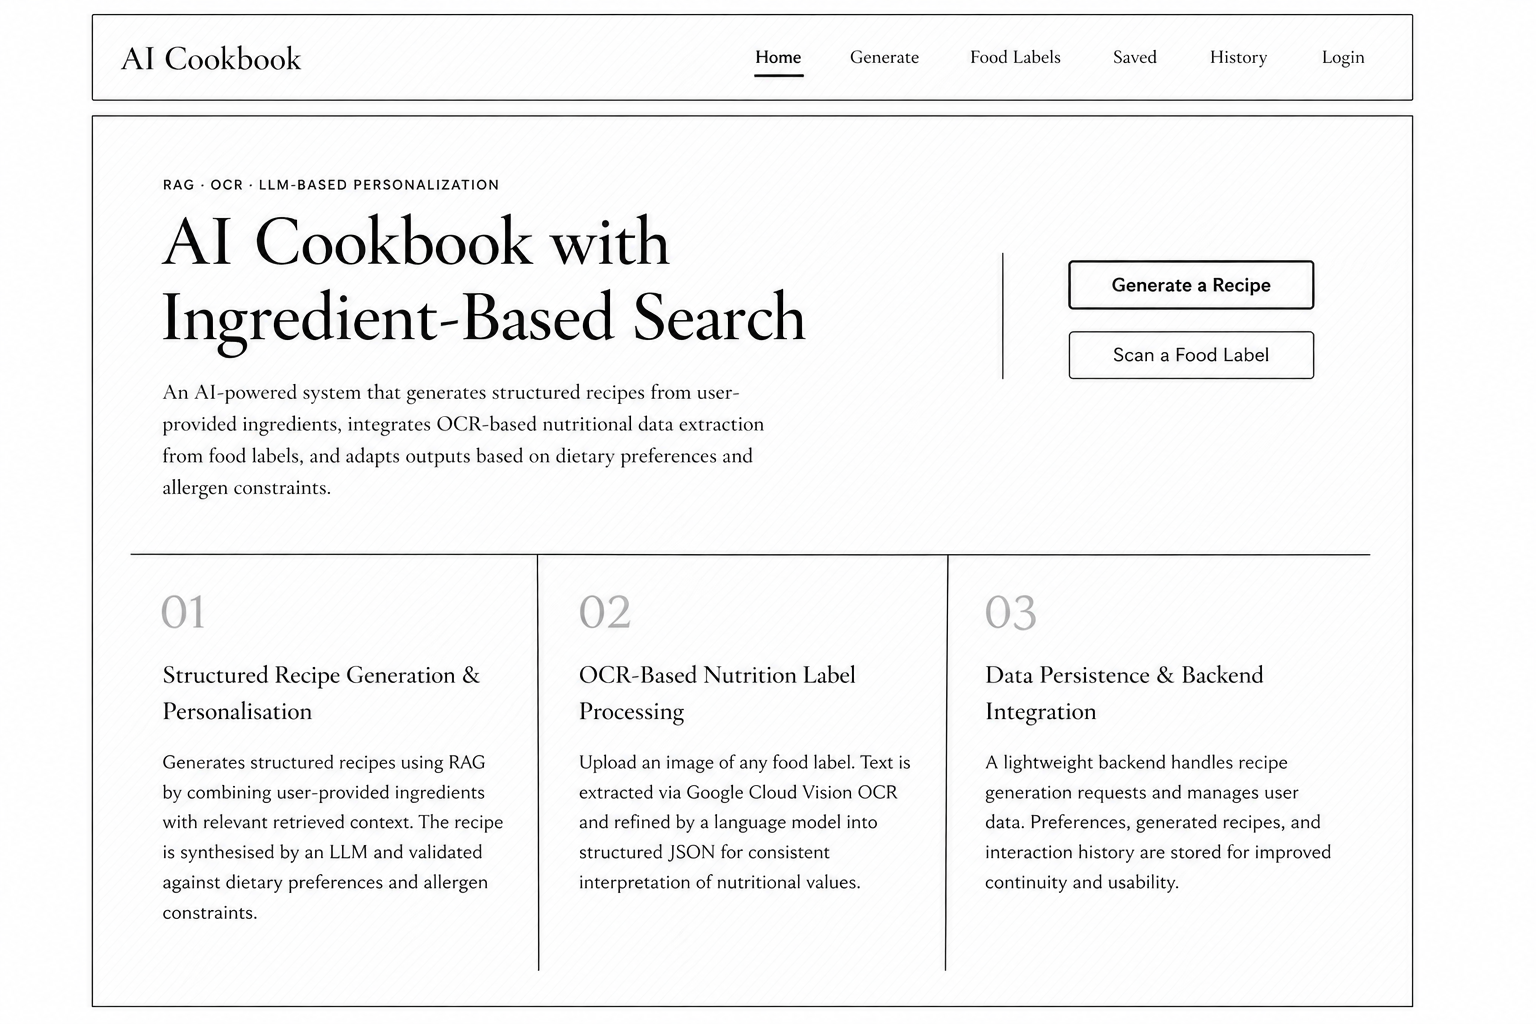
\includegraphics[width=\textwidth]{images/UI/HomeWireframe.png}
		\caption{Home page wireframe}
	\end{subfigure}
	\hfill
	\begin{subfigure}[t]{0.48\textwidth}
		\centering
		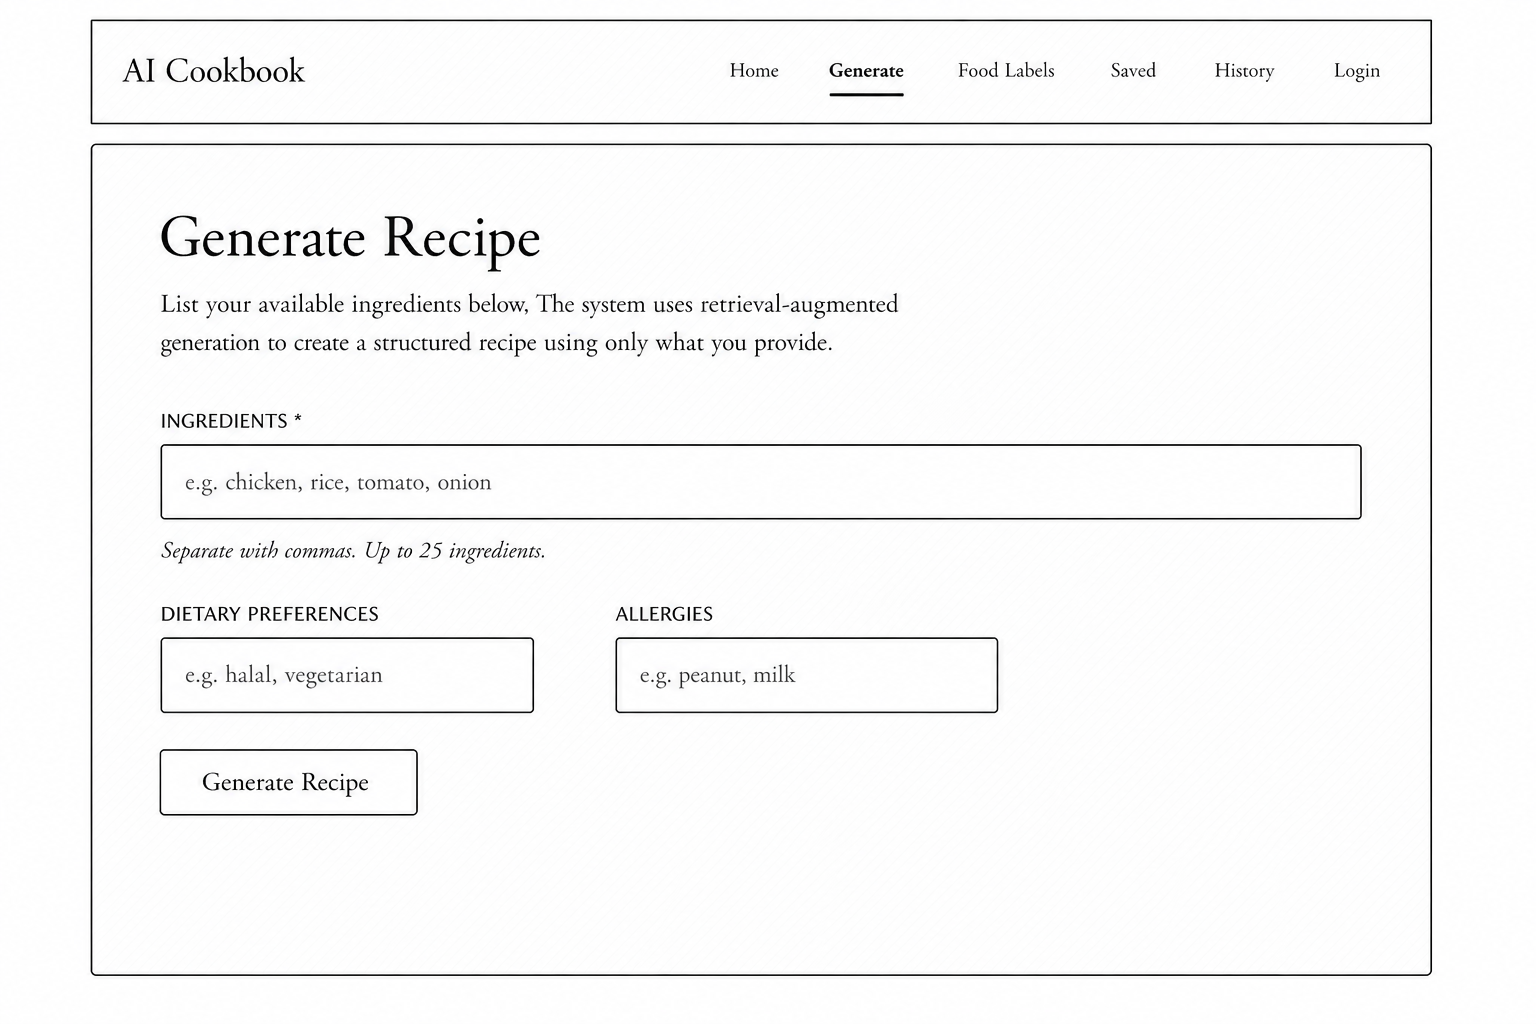
\includegraphics[width=\textwidth]{images/UI/GenerateWireframe.png}
		\caption{Generate page wireframe}
	\end{subfigure}

	\vspace{0.8em}

	\begin{subfigure}[t]{0.48\textwidth}
		\centering
		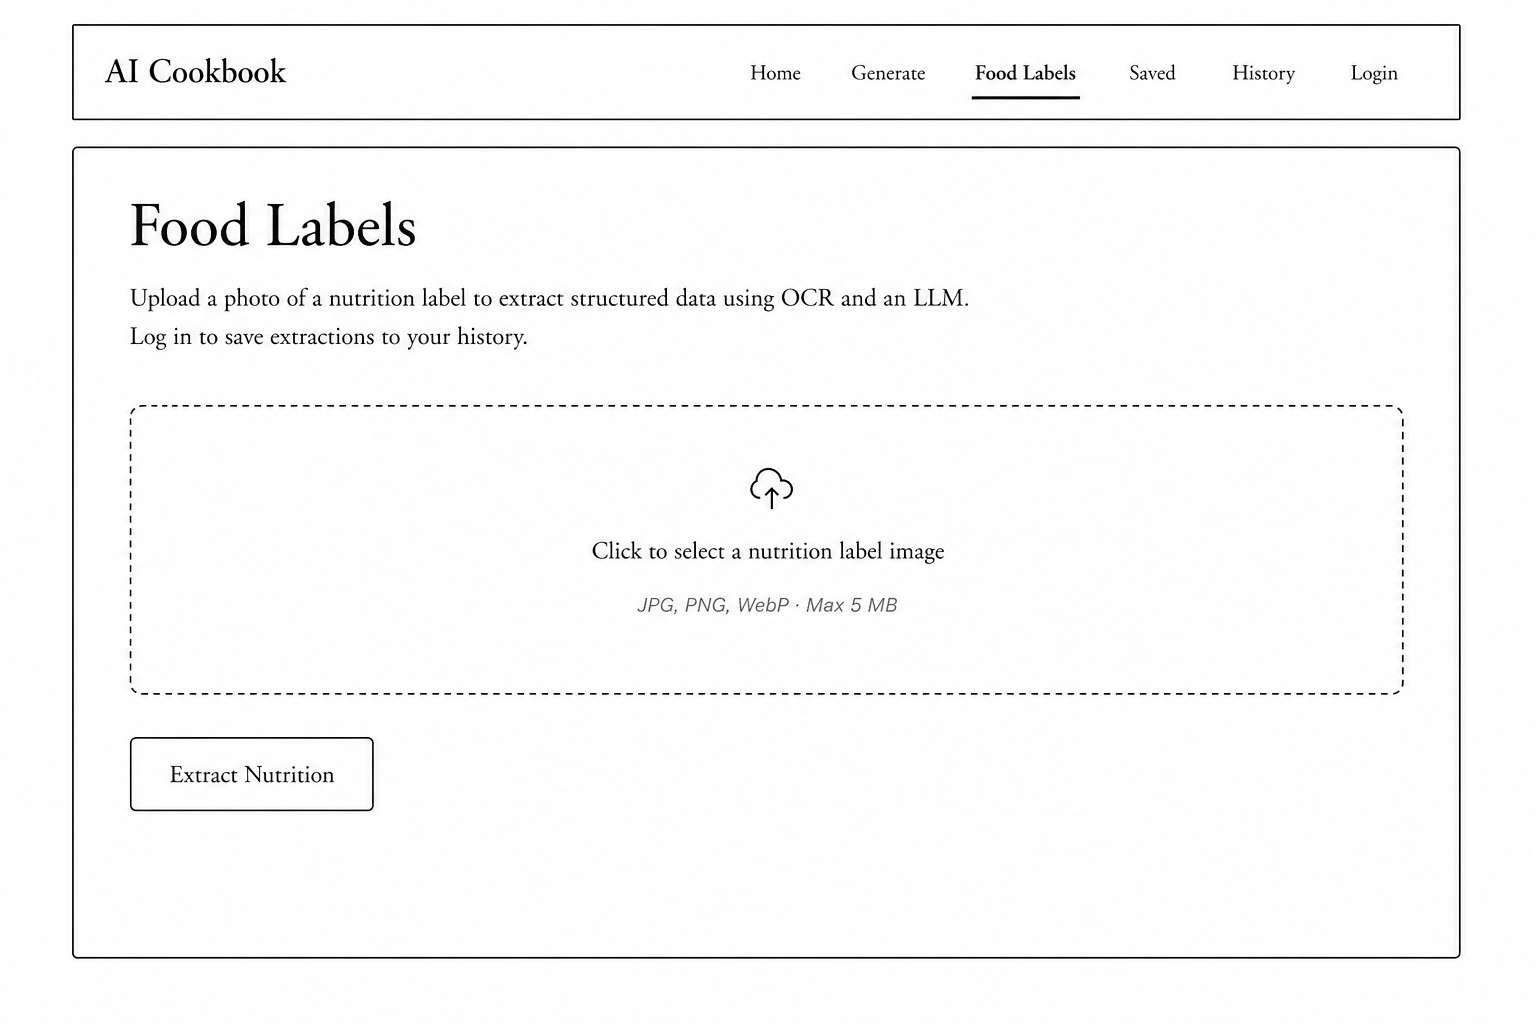
\includegraphics[width=\textwidth]{images/UI/OCRWireframe.png}
		\caption{Food Labels page wireframe}
	\end{subfigure}
	\hfill
	\begin{subfigure}[t]{0.48\textwidth}
		\centering
		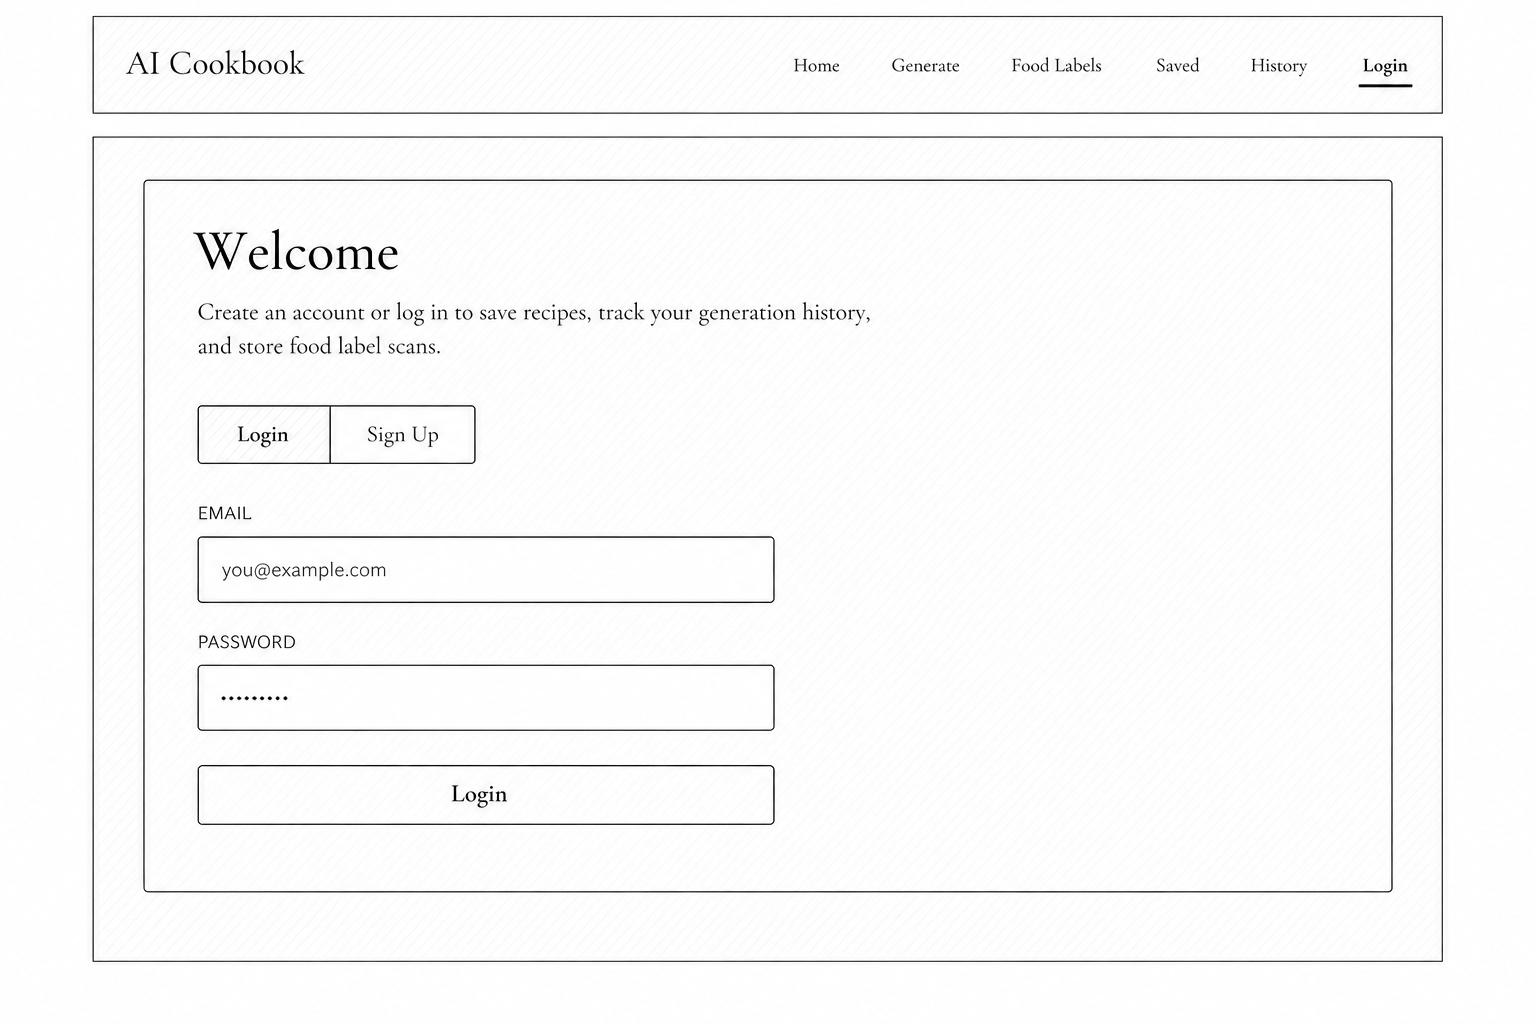
\includegraphics[width=\textwidth]{images/UI/LoginWireframe.png}
		\caption{Login page wireframe}
	\end{subfigure}
	\caption{Primary design-stage wireframes of the main entry and task-oriented pages}
	\label{fig:design-wireframes-main}
\end{figure}

\begin{figure}[p]
	\centering
	\begin{subfigure}[t]{0.48\textwidth}
		\centering
		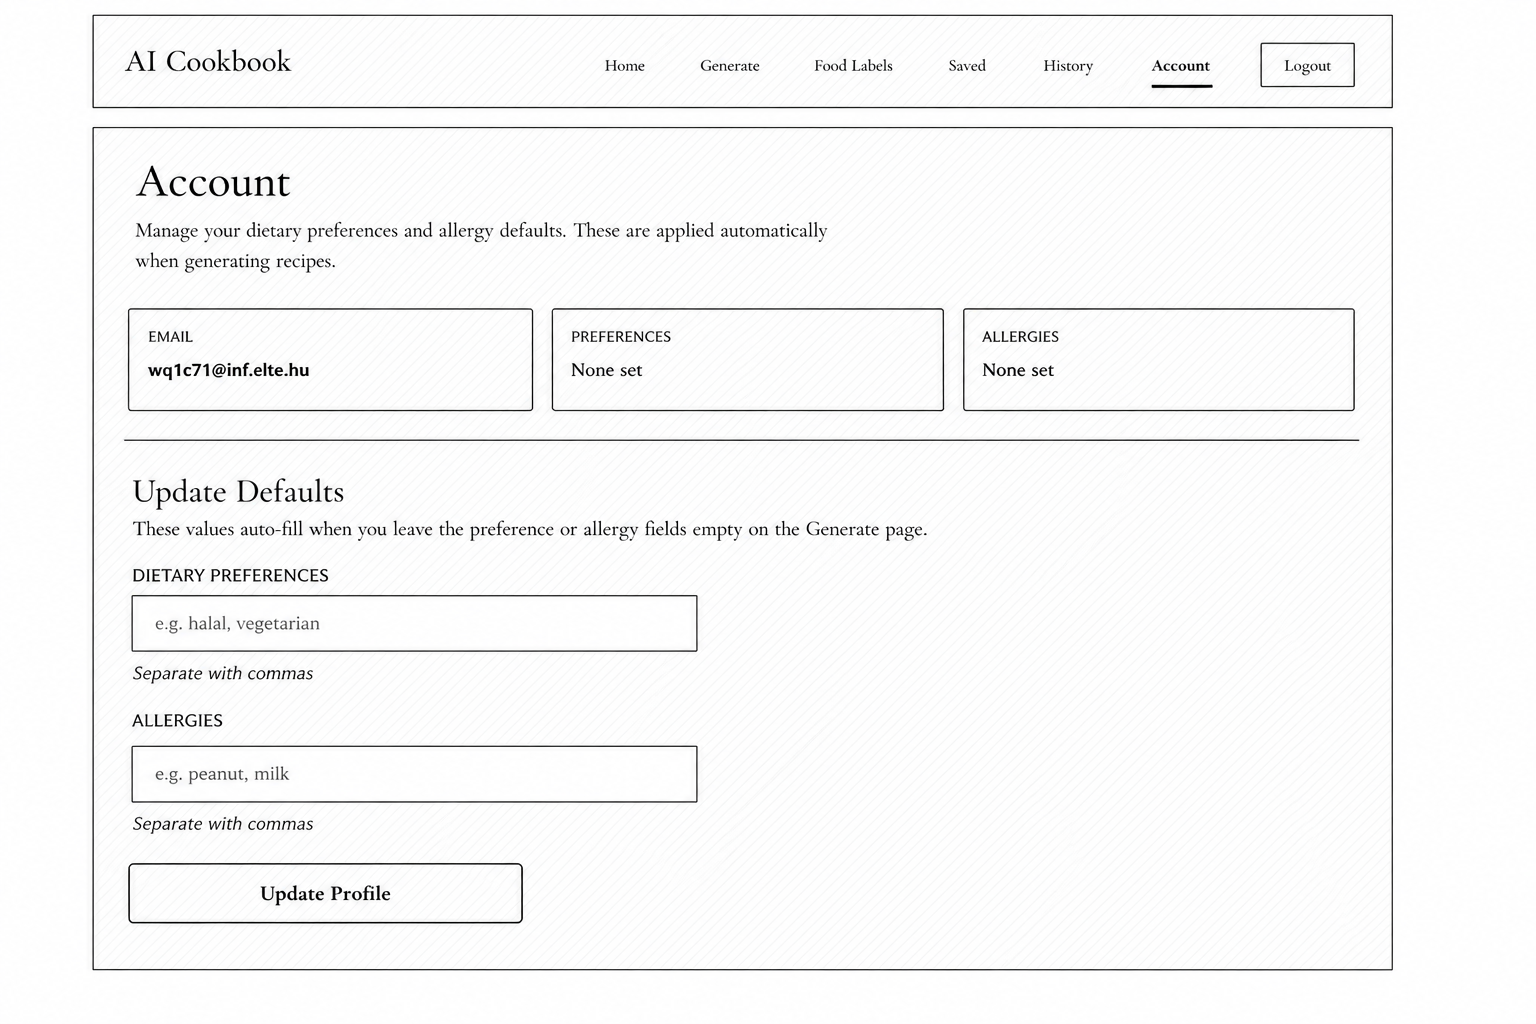
\includegraphics[width=\textwidth]{images/UI/AccountWireframe.png}
		\caption{Account page wireframe}
	\end{subfigure}
	\hfill
	\begin{subfigure}[t]{0.48\textwidth}
		\centering
		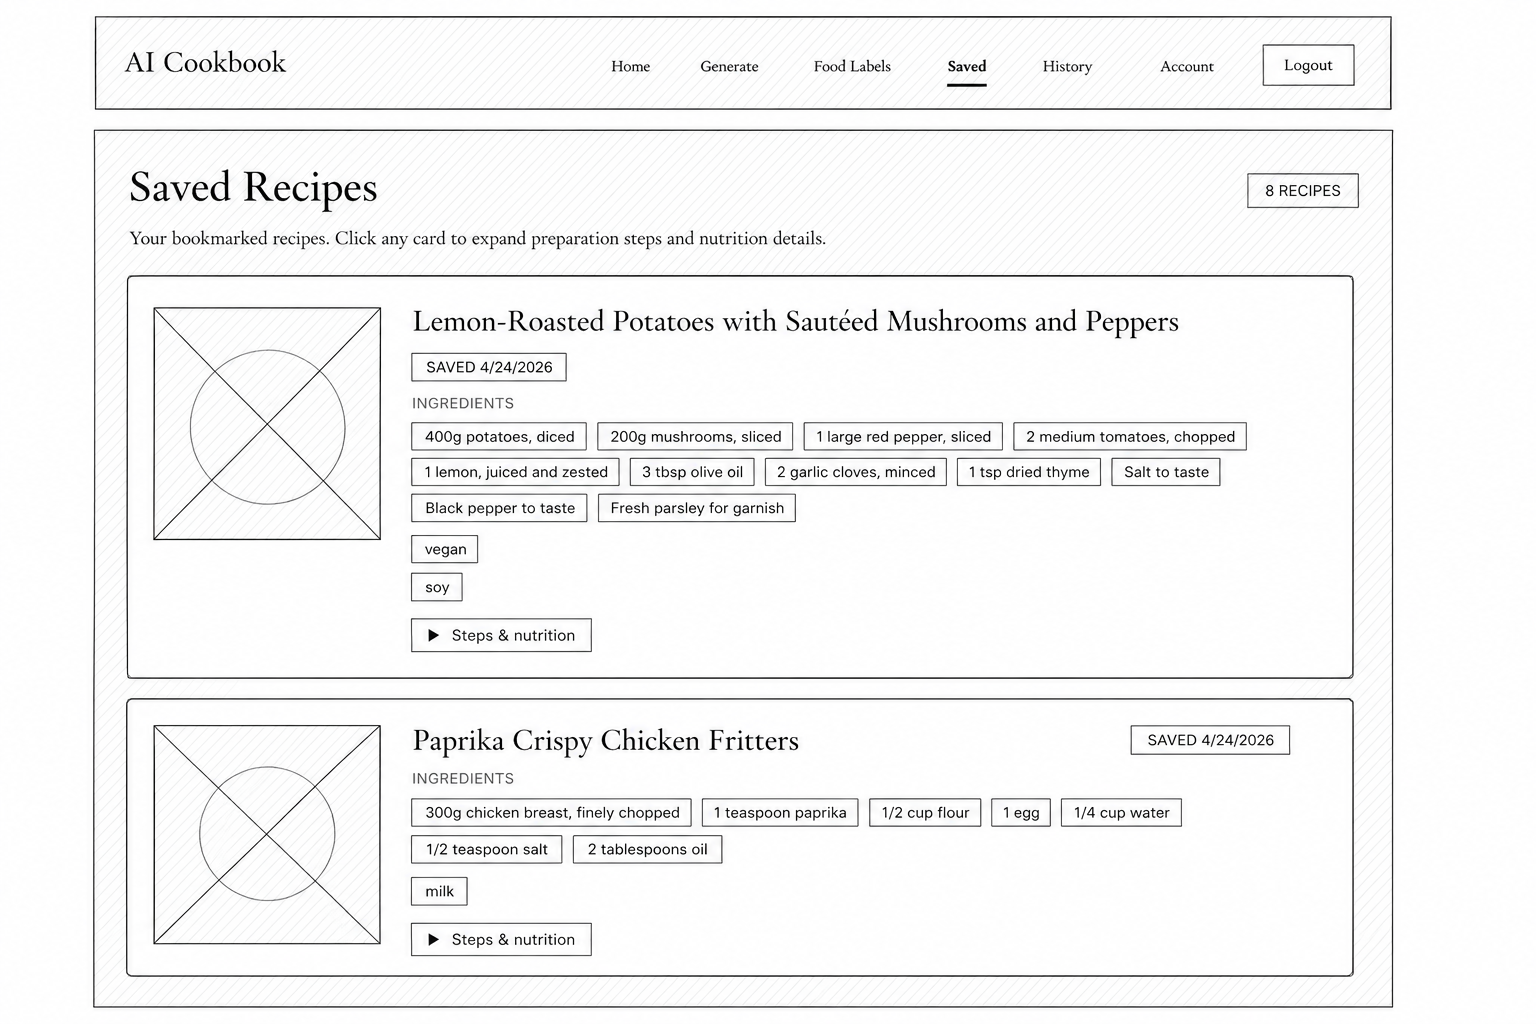
\includegraphics[width=\textwidth]{images/UI/SavedWireframe.png}
		\caption{Saved recipes page wireframe}
	\end{subfigure}

	\vspace{0.8em}

	\begin{subfigure}[t]{0.48\textwidth}
		\centering
		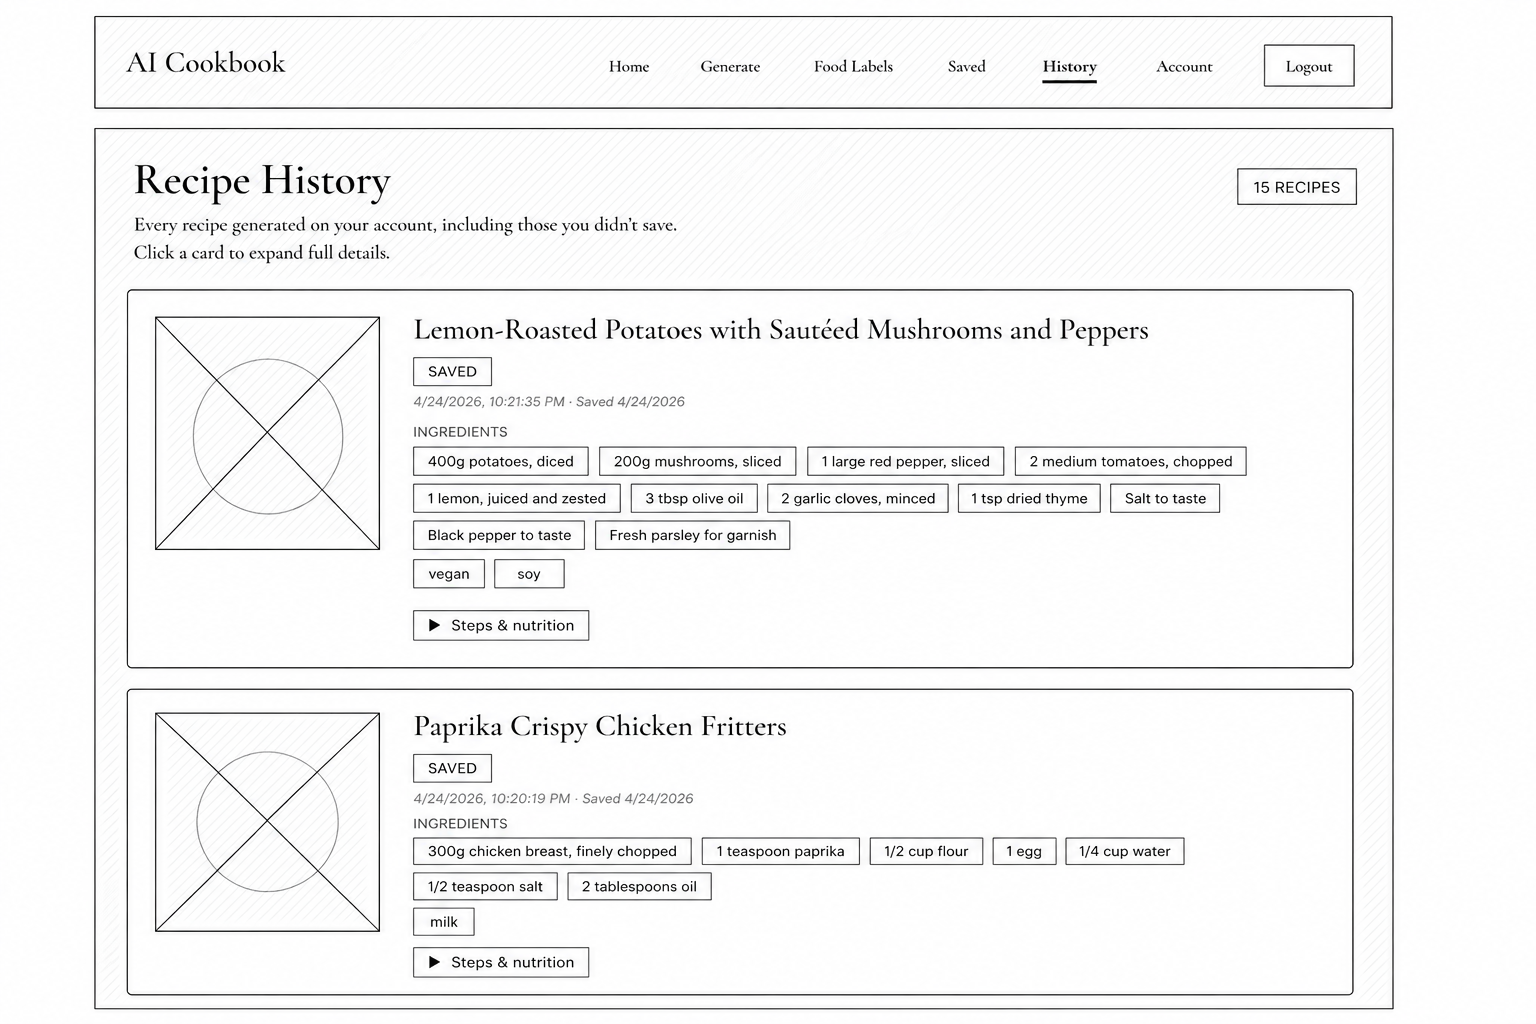
\includegraphics[width=\textwidth]{images/UI/HistoryWireframe.png}
		\caption{History page wireframe}
	\end{subfigure}
	\caption{Secondary design-stage wireframes for persistence and account-related pages}
	\label{fig:design-wireframes-secondary}
\end{figure}

These wireframes already show the three UI decisions that most strongly
influenced the implementation. First, the Generate page reserves space
for dietary constraints near the ingredient input because those
constraints directly shape the generation workflow and warning logic.
Second, recipe warnings deserve a visible zone in the result card
because they communicate safety-relevant information rather than merely
cosmetic status messages. Third, the Food Labels page shows raw OCR text
and the structured nutrition result within the same task view so that
the user can verify how the extraction was interpreted. Finally, save
actions are attached to the result views rather than hidden in secondary
menus, because persistence is a continuation of the primary task rather
than a separate administrative action.

\subsubsection{Navigation structure}

The user interface is organized around a small number of stable routes.
This reduces navigation complexity and makes the main features visible
from the top-level navigation bar.

\begin{itemize}
	\item Home page for overview and entry.
	\item Generate page for recipe-generation tasks.
	\item Food Labels page for OCR extraction tasks.
	\item Saved page for bookmarked recipes.
	\item History page for all generated recipes.
	\item Login / Account page for authentication and default settings.
\end{itemize}

The navigation structure is intentionally task-oriented. Generation,
OCR, persistence, and profile management each have a dedicated visible
location instead of being merged into a single crowded interface.

\subsubsection{Screen-flow design}

\begin{figure}[H]
	\centering
	\resizebox{\textwidth}{!}{
	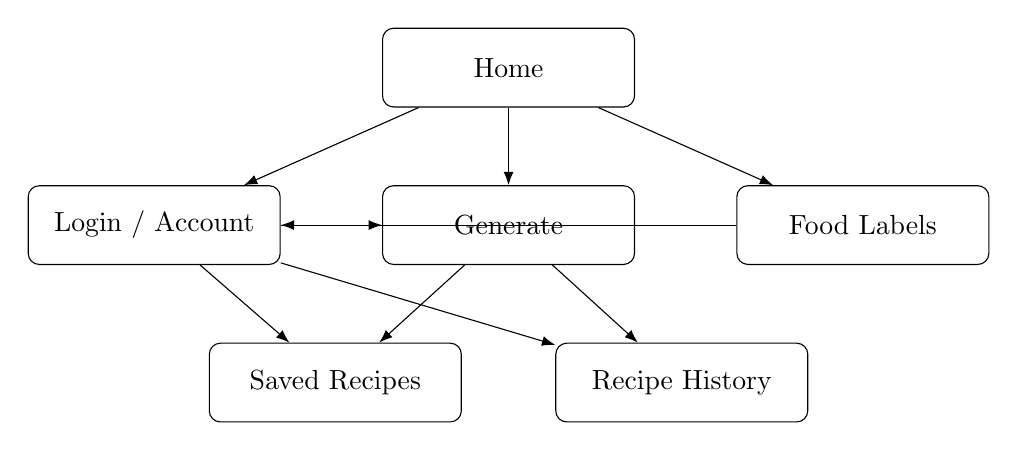
\begin{tikzpicture}[
		screen/.style={draw, rounded corners, minimum width=3.2cm, minimum height=1.0cm, align=center},
		>=Latex
	]
	\node[screen] (home) at (0,0) {Home};
	\node[screen] (login) at (-4.5,-2.0) {Login / Account};
	\node[screen] (gen) at (0,-2.0) {Generate};
	\node[screen] (ocr) at (4.5,-2.0) {Food Labels};
	\node[screen] (saved) at (-2.2,-4.0) {Saved Recipes};
	\node[screen] (hist) at (2.2,-4.0) {Recipe History};

	\draw[-Latex] (home) -- (login);
	\draw[-Latex] (home) -- (gen);
	\draw[-Latex] (home) -- (ocr);
	\draw[-Latex] (login) -- (gen);
	\draw[-Latex] (login) -- (saved);
	\draw[-Latex] (login) -- (hist);
	\draw[-Latex] (gen) -- (saved);
	\draw[-Latex] (gen) -- (hist);
	\draw[-Latex] (ocr) -- (login);
	\end{tikzpicture}}
	\caption{Navigation and screen-transition map of the main frontend pages}
	\label{fig:design-screen-flow}
\end{figure}

\subsubsection{Interaction design decisions}

Three interaction decisions are especially important at design level.

First, recipe-generation warnings are shown prominently in the result
view because they communicate safety-related information about excluded
ingredients, dietary conflicts, and missing thumbnails.

Second, the OCR page shows both the raw extracted text and the
structured nutrition result. This makes the transformation visible to
the user and supports trust, debugging, and manual verification.

Third, saved recipes and full recipe history are separated into
different pages because they represent different user intentions.
Saved recipes act as a curated personal collection, while history acts
as a chronological activity log.

\subsection{Design alternatives considered}

Several alternative designs were considered, but the final choices were
shaped by the scope of the thesis and by what needed to be implemented
and evaluated clearly.

The first alternative was to use a single-prompt language-model
approach for recipe generation without retrieval grounding. That design
would have been simpler to implement, but it would also have made the
generation process less controllable and less tied to an explicit recipe
knowledge base. Retrieval-augmented generation was chosen because it
creates a stronger connection between user input, reusable corpus
content, and the final prompt while still remaining manageable within
the thesis scope.

The second alternative was to process nutrition labels through one
end-to-end image-to-JSON step. The chosen design instead separates OCR
from semantic structuring. This produces a clearer workflow, supports
debugging through raw OCR text, and makes failure causes easier to
locate when the image-processing and interpretation stages behave
differently.

The third alternative was to use fully cloud-oriented persistence for
the relational database, vector store, and media assets. The project
instead keeps SQLite, Chroma persistence, and local media directories.
This local-storage design is appropriate for a thesis because it keeps
deployment reproducible, reduces infrastructure overhead, and still
demonstrates the architectural responsibilities clearly.

The fourth alternative was to require authentication for every feature.
The chosen guest-plus-authenticated model supports easier exploration of
the main AI-supported workflows while still reserving personal history
and profile persistence for authenticated users. This makes the system
easier to demonstrate and test without weakening the ownership model for
private data.

\subsection{Section Summary}

The design chapter establishes the AI Cookbook as a modular
AI-assisted web application with explicit requirements, a layered
architecture, and a mixed persistence strategy. The use-case,
component, class, sequence, state-transition, data-flow, ER, relational
schema, navigation, and wireframe figures document the system from
complementary viewpoints instead of relying on a single diagram type.

The chapter also makes the project-specific rationale explicit: recipe
generation is implemented as a constrained RAG pipeline rather than as a
single prompt call, OCR is split into optical extraction and semantic
structuring, relational persistence is kept intentionally compact, and
the user interface is organized around a small set of dedicated task
pages. This design forms the basis for the implementation chapter, where
these abstractions are mapped to the final modules and code.

\cleardoublepage

\section{Implementation}
\label{ch:implementation}

This section shows how the design from Section~\ref{sec:design} appears in the
codebase. It connects the class, sequence, component, and data design
artifacts to the implemented backend and frontend modules so that the
design decisions can be checked against the actual source code.

\subsection{Development environment and technology stack}

The project is implemented as a monorepo with separate backend and
frontend runtimes. The backend uses Python~3 and FastAPI~0.133.1
\cite{python2026setup,fastapi2026docs}, SQLAlchemy~2.0.48 and
Alembic~1.7.7 \cite{sqlalchemy2026docs,alembic2026docs},
ChromaDB~1.5.5, OpenAI~2.26.0, and Google Cloud Vision~3.11.0
\cite{chromadb2026docs,openai2026platform,google2026vision}, and
Pillow~12.0.0, Pydantic~2.12.5, Pydantic Settings~2.12.5, and
Uvicorn~0.41.0
\cite{pillow2026docs,pydantic2026docs,pydanticsettings2026docs,uvicorn2026docs}.
The frontend uses React~19.2.0, React Router DOM~7.13.1, and
Vite~7.3.1 \cite{react2026docs,reactrouter2026docs,vite2026docs}.
These exact versions are defined in \texttt{backend/requirements.txt}
and \texttt{frontend/package.json}, which makes the implementation
reproducible instead of describing only a generic stack.

The development environment was intentionally lightweight and local.
Source code was edited primarily in Visual Studio Code
\cite{vscode2026docs}, while Git \cite{git2026docs} was used for
version control across both frontend and backend changes. The backend
runtime was managed through a Python virtual environment
and the dependency manifest in
\texttt{backend/requirements.txt}. The frontend runtime was managed
through Node.js and npm \cite{node2026docs,npm2026docs} and the
dependency manifests \texttt{frontend/package.json} and
\texttt{frontend/package-lock.json}. Database schema evolution was
handled through Alembic migration files.

The technology choices follow the layered architecture from
Section~3.2. FastAPI supports thin route modules with built-in request
validation. SQLAlchemy and Alembic realize the relational model in
code. React and Vite support the page-oriented frontend structure, and
ChromaDB makes retrieval part of the working system instead of a design
idea described only on paper.

\subsection{Repository structure and code organization}

The repository structure makes the architectural decomposition visible
before reading individual modules:

\begin{lstlisting}[caption={Repository structure of the implemented system},label={lst:repo-tree}]
ai-cookbook-thesis/
|-- backend/
|   |-- main.py
|   |-- config.py
|   |-- database.py
|   |-- dependencies.py
|   |-- models.py
|   |-- schemas.py
|   |-- security.py
|   |-- rate_limit.py
|   |-- routes/
|   |   |-- auth.py
|   |   |-- ocr.py
|   |   |-- rag_debug.py
|   |   `-- recipes.py
|   |-- services/
|   |   |-- embedding_service.py
|   |   |-- llm_service.py
|   |   |-- ocr_image_processing.py
|   |   |-- ocr_provider.py
|   |   |-- ocr_service.py
|   |   |-- recipe_image_provider.py
|   |   |-- recipe_image_service.py
|   |   |-- rag_service.py
|   |   `-- vector_store_service.py
|   |-- scripts/
|   |   |-- prepare_recipes.py
|   |   `-- index_recipes.py
|   |-- tests/
|   `-- requirements.txt
|-- frontend/
|   |-- package.json
|   `-- src/
|       |-- App.jsx
|       |-- context/AuthContext.jsx
|       |-- lib/api.js
|       |-- components/NutritionGrid.jsx
|       `-- pages/
|           |-- GenerateRecipePage.jsx
|           |-- NutritionPage.jsx
|           |-- SavedRecipesPage.jsx
|           |-- RecipeHistoryPage.jsx
|           `-- LoginPage.jsx
`-- alembic/
    |-- env.py
    `-- versions/
\end{lstlisting}

Table~\ref{tab:repo-directories} summarizes the purpose of the main
directories and shows how the repository structure reflects the
implemented architecture.

\begin{table}[H]
	\centering
	\scriptsize
	\renewcommand{\arraystretch}{1.2}
	\begin{tabular}{|p{3.4cm}|p{10.5cm}|}
		\hline
		\textbf{Directory or area} & \textbf{Purpose in the project} \\
		\hline
		\texttt{backend/} & Contains the server-side application, including routing, validation, business logic, persistence, security, and integration with retrieval and external AI services. \\
		\hline
		\texttt{backend/routes/} & Defines the HTTP entry points for authentication, recipe generation, recipe persistence, OCR extraction, and debugging-oriented retrieval access. \\
		\hline
		\texttt{backend/services/} & Holds the multi-step workflow logic for recipe generation, retrieval, OCR, image handling, and provider abstraction so that route handlers remain thin. \\
		\hline
		\texttt{backend/scripts/} & Contains offline preparation utilities used to clean the recipe corpus and build the persistent retrieval index. \\
		\hline
		\texttt{backend/tests/} & Stores automated backend tests for routes, validation, security behavior, and service-level logic. \\
		\hline
		\texttt{frontend/} & Contains the browser-facing application, its dependency manifest, and the React source used for the main user workflows. \\
		\hline
		\texttt{frontend/src/pages/} & Implements the top-level task pages such as recipe generation, OCR extraction, saved recipes, history, and login/account management. \\
		\hline
		\texttt{frontend/src/components/} & Stores reusable presentation elements shared across pages, such as structured result display components. \\
		\hline
		\texttt{frontend/src/context/} & Maintains shared frontend state, most importantly authentication state and current-profile information. \\
		\hline
		\texttt{frontend/src/lib/} & Groups client-side utility code for API access and URL construction so that request logic is not duplicated across pages. \\
		\hline
		\texttt{alembic/} and \texttt{alembic/versions/} & Store migration configuration and revision history for relational schema changes, keeping database evolution explicit and reproducible. \\
		\hline
	\end{tabular}
	\caption{Purpose of the main repository directories}
	\label{tab:repo-directories}
\end{table}

This file system mirrors the layered design from Section~\ref{sec:design}. Route
modules act as a thin API boundary, service modules contain business
logic and provider orchestration, schema classes define validated data
contracts, and ORM models implement persistence. This is also the point
where the service-orchestration boundary described in the design chapter
becomes visible:
\texttt{routes/recipes.py} exposes one endpoint to the client, while
multiple service modules collaborate behind that boundary.

\subsubsection{Development workflow and repository discipline}

The development workflow was organized around small, feature-oriented
changes rather than large monolithic rewrites. Backend services, API
routes, migrations, frontend pages, and tests were versioned together in
the same repository so that every non-trivial feature could be traced as
one coherent change set. In practice, this was especially important for
features that crossed multiple layers, such as profile-default-aware
recipe generation or OCR history persistence, because they required
coordinated updates in route logic, schemas, frontend state handling,
and tests.

Version-control work followed the same feature-oriented structure.
Changes were developed as focused units around one task or one related
set of tasks instead of mixing unrelated edits into the same revision.
For example, a persistence-related change typically combined the route
logic, schema updates, frontend integration, and migration file needed
for that feature. This kept the history easier to review and reduced the
risk of partial changes that would compile but leave one layer out of
sync with the others.

Dependency and environment management were also repository-driven. The
backend dependency set is declared in
\texttt{backend/requirements.txt}, frontend dependencies in
\texttt{frontend/package.json}, and environment-dependent settings are
centralized through the backend configuration layer and the
\texttt{.env} file format. Database evolution is versioned explicitly
through Alembic revision files instead of implicit schema changes. This
workflow keeps the implementation reproducible: a given repository state
contains not only application code, but also the dependency manifests,
migration history, and indexing scripts needed to reconstruct the
working system.

\subsection{Core application logic and complex features}

This section focuses on the implementation of the main complex features
promised in the project proposal. The first two are the structured
recipe-generation workflow and the OCR-based nutrition-label workflow.
The third, data persistence and backend integration, is covered in
detail later in this section because it spans relational schema design,
ORM mapping, migration history, and query behavior.

\subsubsection{Application bootstrap and request entry points}

The backend entry point is \texttt{backend/main.py}. It does more than
create a FastAPI object: it prepares the runtime environment, installs
cross-cutting middleware, mounts media storage, and registers feature
routers \cite{fastapi2026docs}. This directly realizes the component
diagram from Figure~3.2.

\begin{lstlisting}[language=Python,caption={FastAPI bootstrap in \texttt{backend/main.py}},label={lst:main-bootstrap}]
app = FastAPI(title="AI Cookbook API")
Path("backend/media").mkdir(parents=True, exist_ok=True)
Path(settings.recipe_thumbnail_directory).mkdir(parents=True, exist_ok=True)
Path(settings.ocr_upload_directory).mkdir(parents=True, exist_ok=True)

app.add_middleware(
    CORSMiddleware,
    allow_origins=[settings.frontend_origin],
    allow_credentials=True,
    allow_methods=["*"],
    allow_headers=["*"],
)
app.add_middleware(
    RateLimitMiddleware,
    default_rule=RateLimitRule(
        max_requests=settings.default_rate_limit_requests,
        window_seconds=settings.default_rate_limit_window_seconds,
    ),
    route_rules={
        "/signup": RateLimitRule(...),
        "/generate-recipe": RateLimitRule(...),
        "/ocr/extract": RateLimitRule(...),
    },
)

app.mount("/media", StaticFiles(directory="backend/media"), name="media")
app.include_router(auth.router)
app.include_router(recipes.router)
app.include_router(ocr.router)
app.include_router(rag_debug.router)
\end{lstlisting}

This bootstrap code mainly provides the shared runtime context for the
feature-specific workflows discussed next. It registers the route groups
and installs the middleware and media handling that those workflows rely
on.

\subsubsection{User-specific defaults and authenticated request context}

Authentication is implemented in three modules that work together:
\texttt{backend/security.py} contains Argon2-backed password hashing
and JWT helpers \cite{argon22026docs,pythonjose2026docs,jwt2015rfc7519},
\texttt{backend/dependencies.py} resolves the current user from the
token, and \texttt{backend/routes/auth.py} exposes the HTTP endpoints.
The hashing and verification calls are implemented as follows:

\begin{lstlisting}[language=Python,caption={Password hashing utilities in \texttt{backend/security.py}},label={lst:auth-hashing}]
password_hash = PasswordHash.recommended()

def hash_password(password: str) -> str:
    return password_hash.hash(password)

def verify_password(plain_password: str, hashed_password: str) -> bool:
    return password_hash.verify(plain_password, hashed_password)
\end{lstlisting}

The dependency that enforces ownership of user-specific data is defined
in \texttt{backend/dependencies.py}:

\begin{lstlisting}[language=Python,caption={JWT-based current-user dependency},label={lst:current-user-dependency}]
oauth2_scheme = OAuth2PasswordBearer(tokenUrl="/token")

def get_current_user(
    token: str = Depends(oauth2_scheme),
    db: Session = Depends(get_db),
) -> User:
    user = _get_user_from_token(token, db)
    if user is None:
        raise credentials_exception
    return user
\end{lstlisting}

This function is the implementation-level counterpart of the ownership
relations in the use-case and class diagrams. Endpoints for saving
recipes, browsing history, and saving OCR results depend on the
resolved \texttt{User} instance instead of trusting client-supplied
identifiers.

Profile defaults are persisted in \texttt{backend/routes/auth.py} and
later reused by the frontend when generation fields are left empty:

\begin{lstlisting}[language=Python,caption={Profile update persistence in \texttt{backend/routes/auth.py}},label={lst:profile-update}]
@router.put("/me", response_model=UserResponse)
def update_current_user_profile(...):
    current_user.preferences = json.dumps(profile.preferences)
    current_user.allergies = json.dumps(profile.allergies)
    db.add(current_user)
    db.commit()
    db.refresh(current_user)
    return _user_to_response(current_user)
\end{lstlisting}

\subsubsection{Structured recipe generation and personalization}

Recipe generation is the most complex workflow in the system. It
combines request validation, safety filtering, retrieval, prompt
construction, output verification, optional image generation, and
persistence. The route in \texttt{backend/routes/recipes.py} acts as a
thin facade: it delegates generation to the language-model service and
thumbnail generation to the image service, then optionally persists the
result for the authenticated user.

Personalization enters the workflow at more than one point. User
preferences and allergies can arrive directly in the request or through
stored profile defaults, and they influence both the initial filtering
step and the later prompt construction.

The first non-trivial step is conflict detection. The service checks
whether user-provided ingredients violate allergy or preference
constraints before retrieval or generation starts:

\begin{lstlisting}[language=Python,caption={Conflict analysis in \texttt{backend/services/llm\_service.py}},label={lst:conflict-analysis}]
allergy_conflicts = find_conflicting_ingredients(
    request.ingredients,
    request.allergies,
)
preference_conflicts = find_preference_conflicting_ingredients(
    request.ingredients,
    request.preferences,
)
safe_ingredients = _remove_conflicting_ingredients(
    request.ingredients,
    conflicting_ingredients,
)

if not safe_ingredients:
    raise HTTPException(
        status_code=status.HTTP_400_BAD_REQUEST,
        detail="All provided ingredients conflict with the selected allergies or dietary preferences.",
    )
\end{lstlisting}

This safety-oriented preprocessing is the concrete implementation of the
restriction logic discussed in Section~\ref{sec:design}. It is also one of the points
where the sequence diagram can be verified against real code.

After filtering, the backend retrieves grounded context from the Chroma
collection \cite{chromadb2026docs}. The retrieval call is implemented
in \texttt{backend/services/rag\_service.py}, and the query vector is
created through the embeddings service \cite{openai2026embeddings}:

\begin{lstlisting}[language=Python,caption={Vector retrieval query in \texttt{backend/services/rag\_service.py}},label={lst:rag-query}]
collection = get_collection()
query_text = build_retrieval_query(request)
query_embedding = create_embeddings([query_text])[0]
response = collection.query(
    query_embeddings=[query_embedding],
    n_results=settings.rag_candidate_count,
    include=["metadatas", "distances"],
)
\end{lstlisting}

The prompt sent to the LLM through the OpenAI API
\cite{openai2026api} is not generic. It is assembled from the
filtered ingredient list, user constraints, and retrieved recipe
context. A shortened version of the prompt builder shows this clearly:

\begin{lstlisting}[language=Python,caption={Prompt construction in \texttt{backend/services/llm\_service.py}},label={lst:recipe-prompt}]
return f"""
You are generating a new recipe for an AI cookbook application.

User ingredients: {ingredient_list}.
Dietary preferences: {", ".join(request.preferences) if request.preferences else "none"}.
Allergies to avoid: {", ".join(request.allergies) if request.allergies else "none"}.

Retrieved recipe context (use only as structural inspiration, do NOT copy ingredients):
{context_block}

Return only valid JSON with this exact structure:
{{
  "title": "string",
  "ingredients": ["string", "string"],
  "preferences": ["string"],
  "allergies": ["string"],
  "steps": ["string", "string", "string"],
  "nutrition_estimate": {{
    "calories": 0,
    "protein": "string",
    "carbs": "string",
    "fat": "string"
  }}
}}
""".strip()
\end{lstlisting}

The implementation does not trust the first model response blindly. It
checks for restriction violations and performs one correction cycle when
necessary:

\begin{lstlisting}[language=Python,caption={Output validation and retry loop in \texttt{backend/services/llm\_service.py}},label={lst:retry-loop}]
messages: list[dict] = [{"role": "user", "content": prompt}]

for _ in range(2):
    response = client.chat.completions.create(
        model=settings.openai_model,
        messages=messages,
        temperature=0.7,
    )
    recipe_text = _strip_code_fences(response.choices[0].message.content or "")
    recipe_json = json.loads(recipe_text)
    last_violations = _find_output_restriction_violations(recipe_json, restrictions)

    if not last_violations:
        additional = _find_ingredient_drift(recipe_json, safe_ingredients)
        recipe_json["additional_ingredients"] = additional
        recipe_json["warnings"] = warnings
        return RecipeResponse.model_validate(recipe_json)

    violation_note = (
        "The previous output violated these rules and must be corrected: "
        + "; ".join(last_violations)
    )
    messages.append({"role": "assistant", "content": recipe_text})
    messages.append({"role": "user", "content": violation_note})
\end{lstlisting}

This retry loop is the strongest implementation evidence that recipe
generation is realized as a fixed multi-stage workflow rather than a
single opaque model call. Validation, retrieval, prompt construction,
output checking, corrective retry, and response shaping appear as
explicit stages in code, which is the implementation-level counterpart
of the workflow diagrams and design rationale from Section~\ref{sec:design}.

The implementation also includes dedicated RAG inspection endpoints in
\texttt{backend/routes/rag\_debug.py}. These endpoints are not part of
the normal browser workflow, but they were useful during development
because they expose the same retrieval pipeline that recipe generation
uses internally. The \texttt{/rag/debug} endpoint returns the generated
retrieval query text, the candidates returned by Chroma, the
allergy-conflict filtering result, the ranking score assigned to each
candidate, and which items were ultimately selected as context. The
\texttt{/rag/collection-stats} endpoint provides a lighter diagnostic
view over the indexed corpus. In practice, these endpoints made it
possible to verify that failures or weak recipe outputs came from
retrieval quality, filtering, or prompt behavior rather than from a
single opaque model response.

\subsubsection{OCR-based nutrition label processing}

The OCR subsystem is implemented as a two-stage pipeline: optical text
recognition followed by semantic structuring into validated nutrition
fields. The abstraction boundary for OCR providers is defined in
\texttt{backend/services/ocr\_provider.py}
\cite{google2026vision}:

\begin{lstlisting}[language=Python,caption={OCR provider strategy in \texttt{backend/services/ocr\_provider.py}},label={lst:ocr-provider}]
class OcrProvider(ABC):
    @abstractmethod
    def extract_text(self, image_bytes: bytes) -> str:
        """Extract raw OCR text from an image payload."""

class GoogleVisionOcrProvider(OcrProvider):
    def extract_text(self, image_bytes: bytes) -> str:
        return extract_text_with_google_vision(image_bytes)

@lru_cache(maxsize=1)
def get_ocr_provider() -> OcrProvider:
    if settings.ocr_provider == "google_vision":
        return GoogleVisionOcrProvider()
\end{lstlisting}

This implements the provider-substitution mechanism described in the
design chapter. The OCR workflow depends on an application-level
interface and can switch concrete providers without changing the route
or higher-level service logic.

Before OCR is executed, images are validated and normalized in
\texttt{backend/services/ocr\_image\_processing.py} with Pillow
\cite{pillow2026docs}:

\begin{lstlisting}[language=Python,caption={Image preprocessing for OCR},label={lst:ocr-preprocess}]
def prepare_image_for_ocr(file_bytes: bytes) -> bytes:
    image = Image.open(BytesIO(file_bytes))
    image.load()

    normalized = ImageOps.exif_transpose(image)
    grayscale = ImageOps.grayscale(normalized)
    contrast_ready = ImageOps.autocontrast(grayscale)
    enlarged = contrast_ready.resize(
        (contrast_ready.width * 2, contrast_ready.height * 2)
    )

    buffer = BytesIO()
    enlarged.save(buffer, format="PNG")
    return buffer.getvalue()
\end{lstlisting}

The second OCR stage turns raw text into structured JSON
\cite{json2017rfc8259}. The LLM prompt shows that the expected schema
is explicit and validated later through Pydantic
\cite{pydantic2026docs}:

\begin{lstlisting}[language=Python,caption={Nutrition-structuring prompt in \texttt{backend/services/ocr\_service.py}},label={lst:ocr-prompt}]
prompt = f"""
You are given OCR text from a food nutrition label.
Extract only the nutrition information you can confidently identify.

Return only valid JSON in this exact structure:
{{
  "product_name": "string or null",
  "serving_size": "string or null",
  "calories": 0,
  "protein_g": 0,
  "carbs_g": 0,
  "fat_g": 0,
  "sugar_g": 0,
  "sodium_mg": 0,
  "fiber_g": 0
}}
""".strip()
\end{lstlisting}

\subsubsection{Supporting image generation and caching}

Recipe thumbnails are generated only after the textual recipe has
already been accepted. The implementation first derives a deterministic
cache key from normalized ingredient data:

\begin{lstlisting}[language=Python,caption={Thumbnail cache key derivation in \texttt{backend/services/recipe\_image\_service.py}},label={lst:image-cache-key}]
def build_recipe_image_cache_key(
    title: str,
    ingredients: list[str],
    preferences: list[str],
    allergies: list[str],
) -> str:
    normalized_ingredients = sorted(
        _normalize_text(item) for item in ingredients if item.strip()
    )
    digest_source = ",".join(normalized_ingredients)
    return hashlib.sha256(digest_source.encode("utf-8")).hexdigest()[:24]
\end{lstlisting}

The cache lookup and provider delegation are implemented in the same
service:

\begin{lstlisting}[language=Python,caption={Thumbnail reuse and generation logic},label={lst:image-cache-lookup}]
thumbnail_path = _get_thumbnail_path(cache_key)

if thumbnail_path.exists():
    return {
        "image_cache_key": cache_key,
        "image_path": str(thumbnail_path.as_posix()),
        "image_url": _to_public_image_url(cache_key),
        "image_prompt": prompt,
    }

image_bytes = get_recipe_image_provider().generate_png(prompt)
thumbnail_path.write_bytes(image_bytes)
\end{lstlisting}

The concrete provider for image generation is again represented through
an abstract interface and a provider-specific implementation
\cite{openai2026images,openai2026api}:

\begin{lstlisting}[language=Python,caption={Recipe image provider in \texttt{backend/services/recipe\_image\_provider.py}},label={lst:image-provider}]
class RecipeImageProvider(ABC):
    @abstractmethod
    def generate_png(self, prompt: str) -> bytes:
        """Generate a PNG image for the given prompt."""

class OpenAIRecipeImageProvider(RecipeImageProvider):
    def generate_png(self, prompt: str) -> bytes:
        response = self._client.images.generate(
            model=settings.openai_image_model,
            prompt=prompt,
            size="1024x1024",
            quality="low",
            output_format="png",
        )
\end{lstlisting}

This code provides supporting infrastructure for the recipe-generation
feature. Thumbnail generation is not the primary feature outcome, but it
improves the usability of generated results and saved-history views
without changing the main textual workflow.

\subsubsection{Request protection}

Request throttling is implemented in \texttt{backend/rate\_limit.py} as
custom middleware instead of an external gateway dependency. The
middleware keeps an in-memory bucket per client and route:

\begin{lstlisting}[language=Python,caption={Rate-limiting middleware structure},label={lst:rate-limit}]
@dataclass(frozen=True)
class RateLimitRule:
    max_requests: int
    window_seconds: int

class RateLimitMiddleware(BaseHTTPMiddleware):
    async def dispatch(self, request: Request, call_next):
        rule = self._resolve_rule(request)
        client_identifier = self._get_client_identifier(request)
        key = f"{request.method}:{request.url.path}:{client_identifier}"
        allowed, retry_after = self.rate_limiter.check(key, rule)

        if not allowed:
            return JSONResponse(
                status_code=429,
                content={"detail": "Rate limit exceeded. Please try again later."},
                headers={"Retry-After": str(retry_after)},
            )
\end{lstlisting}

The route-specific limits visible earlier in Listing~\ref{lst:main-bootstrap}
show that authentication, recipe generation, and OCR extraction are
protected more strictly than ordinary reads. This is a concrete example
of a cross-cutting concern being realized in middleware rather than
inside every individual route function.

\subsection{Frontend implementation}

\subsubsection{Application shell and routing}

The frontend is organized as a React single-page application whose
top-level router maps directly to the main workflows from the use-case
and navigation diagrams. The routes are declared in
\texttt{frontend/src/App.jsx}, while each major use case is implemented
as its own page component under \texttt{frontend/src/pages/}. This
keeps the frontend aligned with the screen-flow diagram from
Section~3.4 and follows the React and React Router application model
\cite{react2026docs,reactrouter2026docs}.

The page organization is intentionally task-oriented. The Home page
provides entry points into the two primary AI-supported workflows,
Generate and Food Labels. The Login/Account page combines
authentication-related interaction with profile-default management, so
the user does not have to navigate to a separate settings area. The
Saved and History pages then separate two different persistence views:
one for explicitly bookmarked recipes and one for the full generation
history. This mirrors the frontend route structure visible in
\texttt{App.jsx} and keeps each page responsible for one coherent user
task.

\subsubsection{Centralized API access}

HTTP communication \cite{http2022rfc9110} is centralized in
\texttt{frontend/src/lib/api.js}. This module provides a single base URL
resolver and a reusable
\texttt{apiFetch()} wrapper that turns non-success responses into
JavaScript errors with backend-supplied detail messages when available.
This design keeps page components focused on user interaction and local
state instead of repeating low-level request boilerplate. It also gives
the frontend one consistent place to adapt API-base configuration across
development environments.

\subsubsection{Authentication state management}

Shared authentication state is implemented through the React context in
\texttt{frontend/src/context/AuthContext.jsx} \cite{react2026docs}:

\begin{lstlisting}[language=Java,caption={Authentication context in \texttt{frontend/src/context/AuthContext.jsx}},label={lst:auth-context}]
const AuthContext = createContext(null);

export function AuthProvider({ children }) {
  const [token, setToken] = useState(() => localStorage.getItem("token"));
  const [profile, setProfile] = useState(null);
  const [profileLoading, setProfileLoading] = useState(false);

  useEffect(() => {
    if (!token) {
      setProfile(null);
      return;
    }

    const loadProfile = async () => {
      const data = await apiFetch("/me", {
        headers: { Authorization: `Bearer ${token}` },
      });
      setProfile(data);
    };

    loadProfile();
  }, [token]);
}
\end{lstlisting}

This module is the frontend counterpart of the backend
\texttt{get\_current\_user} dependency. The context stores the token,
loads the user profile from \texttt{/me}, and exposes state that other
pages use to decide whether save actions or account-aware defaults are
available.

\subsubsection{Recipe-generation page}

The most interesting frontend behavior is the fallback from manual
fields to stored profile defaults. It is implemented directly in
\texttt{frontend/src/pages/GenerateRecipePage.jsx}:

\begin{lstlisting}[language=Java,caption={Profile-default fallback on the generation page},label={lst:profile-fallback-frontend}]
const manualPreferences = preferences.split(",").map((i) => i.trim()).filter(Boolean);
const manualAllergies = allergies.split(",").map((i) => i.trim()).filter(Boolean);

const payload = {
  ingredients: parsedIngredients,
  preferences: manualPreferences.length > 0 ? manualPreferences : profile?.preferences || [],
  allergies: manualAllergies.length > 0 ? manualAllergies : profile?.allergies || [],
};
\end{lstlisting}

This short block is an important implementation detail because it shows
how profile management and recipe generation are connected across the
frontend and backend. The feature was discussed in the design chapter,
but here it becomes visible as a concrete data-flow decision.

The same page also shows how the generated recipe identifier is used to
persist a bookmarked recipe only after successful generation:

\begin{lstlisting}[language=Java,caption={Saving a generated recipe from the frontend},label={lst:save-recipe-frontend}]
await apiFetch("/recipes", {
  method: "POST",
  headers: {
    "Content-Type": "application/json",
    Authorization: `Bearer ${token}`,
  },
  body: JSON.stringify({ generated_recipe_id: recipe.generated_recipe_id }),
});
\end{lstlisting}

The same page also illustrates the frontend state pattern used
throughout the application: input state is kept locally, asynchronous
actions toggle explicit loading flags, and result or error state is
rendered conditionally. Recipe generation, OCR extraction, profile
updates, and history loading all follow this same approach, which keeps
page behavior easy to reason about without introducing a heavier global
state solution.

\subsubsection{OCR and history-oriented pages}

The Food Labels page combines upload interaction, OCR result rendering,
save behavior, and paginated history loading in a single task-oriented
view. After the user selects an image, the page constructs a
\texttt{FormData} payload for \texttt{/ocr/extract}, renders the raw OCR
text together with the structured nutrition result, and conditionally
enables saving when the user is authenticated. The page also loads
saved OCR history through page-number and page-size query parameters,
which makes the backend pagination contract visible in the frontend.

The Saved Recipes page and Recipe History page follow the same
data-access pattern. Both request paginated backend data, maintain local
\texttt{loading}, \texttt{error}, \texttt{page}, and
\texttt{totalPages} state, and render pagination controls only when more
than one page exists. The difference is semantic rather than structural:
the Saved page filters for explicitly bookmarked recipes, while the
History page displays all generated recipe entries, including unsaved
ones and their warnings. This close structural similarity is useful
because it keeps persistence-related pages consistent for the user while
still preserving their different purposes.

\subsubsection{Structured result presentation}

Structured nutritional output is rendered through the reusable
\texttt{frontend/src/components/NutritionGrid.jsx} component. The
component accepts a nutrition object and an optional field list, which
allows the same grid to display the compact recipe nutrition estimate on
the Generate, Saved, and History pages, and the richer OCR nutrition
schema on the Food Labels page. This is a small but meaningful frontend
abstraction: presentation logic for structured nutrition data is kept in
one component instead of being duplicated across multiple pages.

\subsection{Persistence implementation}

\subsubsection{Relational schema in executable form}

The relational design from Section~\ref{sec:design} is not only diagrammed; it is
materialized through ORM mappings and migration files. The resulting
tables remain small in number but rich enough to capture ownership,
save-state transitions, timestamps, and the denormalized structured
payloads returned by the application. The following DDL-style excerpt
shows the schema shape that the ORM and Alembic revisions realize
\cite{sqlalchemy2026docs,alembic2026docs}:

\begin{lstlisting}[language=SQL,caption={Representative relational DDL for the implemented schema},label={lst:ddl-schema}]
CREATE TABLE users (
    id INTEGER PRIMARY KEY,
    email VARCHAR NOT NULL UNIQUE,
    password VARCHAR NOT NULL,
    preferences TEXT NOT NULL DEFAULT '[]',
    allergies TEXT NOT NULL DEFAULT '[]',
    created_at DATETIME DEFAULT CURRENT_TIMESTAMP
);

CREATE TABLE generated_recipes (
    id INTEGER PRIMARY KEY,
    fingerprint VARCHAR NOT NULL,
    title VARCHAR NOT NULL,
    ingredients TEXT NOT NULL,
    additional_ingredients TEXT NOT NULL DEFAULT '[]',
    preferences TEXT NOT NULL DEFAULT '[]',
    allergies TEXT NOT NULL DEFAULT '[]',
    steps TEXT NOT NULL,
    nutrition TEXT NOT NULL,
    warnings TEXT NOT NULL DEFAULT '[]',
    image_url VARCHAR,
    image_path VARCHAR,
    image_cache_key VARCHAR,
    image_prompt TEXT,
    is_saved BOOLEAN NOT NULL DEFAULT FALSE,
    saved_at DATETIME,
    created_at DATETIME DEFAULT CURRENT_TIMESTAMP,
    user_id INTEGER REFERENCES users(id)
);

CREATE TABLE ocr_extractions (
    id INTEGER PRIMARY KEY,
    source_filename VARCHAR NOT NULL,
    raw_text TEXT NOT NULL,
    structured_nutrition TEXT NOT NULL,
    image_path VARCHAR,
    image_url VARCHAR,
    created_at DATETIME DEFAULT CURRENT_TIMESTAMP,
    user_id INTEGER NOT NULL REFERENCES users(id)
);
\end{lstlisting}

This representation is useful because it makes the key decisions
visible in one place: the ownership model is implemented through foreign
keys, recipe persistence permits a nullable owner because guest
generation exists conceptually, and structured variable-length content
is stored as serialized text rather than decomposed into many auxiliary
tables.

The \texttt{fingerprint} field in \texttt{generated\_recipes} is also an
implementation detail with practical value rather than a decorative
schema element. In \texttt{backend/utils.py}, the application builds
this fingerprint by normalizing the recipe title, ingredients,
preferences, allergies, and steps, serializing the normalized payload,
and hashing it with SHA-256. This makes the identity
of a generated recipe depend on its meaningful content instead of
surface formatting differences such as extra whitespace or input order.
The result is a stable identifier that can be stored together with the
generated row and reused in later comparisons or debugging.

\subsubsection{ORM entities}

The relational model from Section~\ref{sec:design} is implemented in
\texttt{backend/models.py} with SQLAlchemy
\cite{sqlalchemy2026docs}. The \texttt{GeneratedRecipe} entity is the
most important example because it combines ownership, save state,
thumbnail metadata, and several intentionally serialized fields:

\begin{lstlisting}[language=Python,caption={\texttt{GeneratedRecipe} ORM mapping},label={lst:generated-recipe-model}]
class GeneratedRecipe(Base):
    __tablename__ = "generated_recipes"

    id = Column(Integer, primary_key=True, index=True)
    fingerprint = Column(String, nullable=False, index=True)
    title = Column(String, nullable=False)
    ingredients = Column(Text, nullable=False)
    additional_ingredients = Column(Text, nullable=False, default="[]")
    preferences = Column(Text, nullable=False, default="[]")
    allergies = Column(Text, nullable=False, default="[]")
    steps = Column(Text, nullable=False)
    nutrition = Column(Text, nullable=False)
    warnings = Column(Text, nullable=False, default="[]")
    image_url = Column(String, nullable=True)
    image_path = Column(String, nullable=True)
    image_cache_key = Column(String, nullable=True, index=True)
    is_saved = Column(Boolean, nullable=False, default=False, server_default="false")
    saved_at = Column(DateTime(timezone=True), nullable=True)
    created_at = Column(DateTime(timezone=True), server_default=func.now())
    user_id = Column(Integer, ForeignKey("users.id"), nullable=True)

    owner = relationship("User", back_populates="generated_recipes")
\end{lstlisting}

This mapping closes the loop between the ER diagram, the relational
schema, and the implementation. The JSON-serialized text fields are a
deliberate denormalization tradeoff already justified in
Section~3.3.4: they simplify storage of variable-length ingredient,
warning, and step lists without introducing multiple auxiliary tables
for a thesis-scale application.

\subsubsection{Schema migration history}

Schema evolution is managed through Alembic \cite{alembic2026docs}. The migration
\texttt{a3f9c2d1e804\_ocr\_image\_fields\_and\_pagination\_indexes.py}
is a good example because it adds both new columns and composite
indexes:

\begin{lstlisting}[language=Python,caption={Alembic revision adding image fields and pagination indexes},label={lst:alembic-indexes}]
def upgrade() -> None:
    op.add_column("ocr_extractions", sa.Column("image_path", sa.String(), nullable=True))
    op.add_column("ocr_extractions", sa.Column("image_url", sa.String(), nullable=True))

    with op.batch_alter_table("generated_recipes") as batch_op:
        batch_op.create_index(
            "ix_generated_recipes_user_saved_at",
            ["user_id", "is_saved", "saved_at"],
        )
        batch_op.create_index(
            "ix_generated_recipes_user_created_at",
            ["user_id", "created_at"],
        )
\end{lstlisting}

This revision demonstrates that the relational design did not remain
static after the ERD was drawn. The database schema evolved together
with the implementation needs of OCR history and paginated history
views.

The same evolution also shows where the implementation became more
precise than the first conceptual sketch. The design stabilized around
three adjustments in particular. First, recipe history and explicit
saved recipes were kept in the same table instead of being split into
two separate persistence models, because save-state is an attribute of a
generated result rather than a different domain object. Second, OCR
history gained image-path and image-URL fields only once the frontend
history view made image recall part of the user-visible workflow.
Third, pagination support led directly to composite indexes on
\texttt{generated\_recipes} and \texttt{ocr\_extractions}, so the final
schema reflects not only domain entities but also the access patterns
that emerged during implementation.

\subsubsection{Query and indexing implementation}

The composite indexes above are used by the saved-recipes and history
queries in \texttt{backend/routes/recipes.py}. The saved-recipes query
is shown below:

\begin{lstlisting}[language=Python,caption={Saved-recipes query using the ownership and save-state fields},label={lst:saved-query}]
base_query = db.query(GeneratedRecipe).filter(
    GeneratedRecipe.user_id == current_user.id,
    GeneratedRecipe.is_saved.is_(True),
)
rows = (
    base_query
    .order_by(GeneratedRecipe.saved_at.desc(), GeneratedRecipe.created_at.desc())
    .offset((page - 1) * page_size)
    .limit(page_size)
    .all()
)
\end{lstlisting}

This query is not only persistence code but also evidence that the
index strategy described in Section~\ref{sec:design} is connected to an actual access
pattern in the system.

The same query can be expressed at SQL level as follows:

\begin{lstlisting}[language=SQL,caption={SQL form of the saved-recipes listing query},label={lst:saved-query-sql}]
SELECT
    id,
    title,
    ingredients,
    additional_ingredients,
    preferences,
    allergies,
    steps,
    nutrition,
    image_url,
    image_cache_key,
    saved_at,
    created_at
FROM generated_recipes
WHERE user_id = :current_user_id
  AND is_saved = TRUE
ORDER BY saved_at DESC, created_at DESC
LIMIT :page_size OFFSET :offset;
\end{lstlisting}

This query uses the same ownership and save-state conditions that
appear in the ORM code and benefits directly from the composite index on
\texttt{(user\_id, is\_saved, saved\_at)}. The ordering also reflects a
domain choice: once a recipe becomes part of the saved collection, the
most relevant timestamp is the save action rather than the original
generation time.

Although the user-facing application mainly executes ownership-scoped
single-table reads, the same relational model also supports more
analytical queries when needed. For example, the following aggregation
query can summarize per-user recipe activity by combining a join,
conditional aggregation, and descending ranking:

\begin{lstlisting}[language=SQL,caption={Analytical SQL over the implemented recipe-history schema},label={lst:activity-aggregation-sql}]
SELECT
    u.email,
    COUNT(gr.id) AS generated_recipe_count,
    SUM(CASE WHEN gr.is_saved = TRUE THEN 1 ELSE 0 END) AS saved_recipe_count,
    MAX(gr.created_at) AS latest_generation_at
FROM users AS u
LEFT JOIN generated_recipes AS gr
    ON gr.user_id = u.id
GROUP BY u.id, u.email
ORDER BY generated_recipe_count DESC, latest_generation_at DESC;
\end{lstlisting}

This query is not part of the current browser workflow, but it is still
important documentation evidence because it shows that the schema
supports not only transactional reads and writes but also higher-level
reporting over the same ownership model.

The retrieval corpus is indexed offline through
\texttt{backend/scripts/index\_recipes.py}:

\begin{lstlisting}[language=Python,caption={Offline recipe-corpus indexing for ChromaDB},label={lst:index-script}]
def index_recipe_corpus() -> None:
    recipes = load_recipe_corpus(corpus_path)
    collection = get_collection()
    existing = collection.get(include=[])
    existing_ids = existing.get("ids", [])
    if existing_ids:
        collection.delete(ids=existing_ids)

    for start in range(0, len(recipes), batch_size):
        batch = recipes[start : start + batch_size]
        documents = [build_recipe_document(recipe) for recipe in batch]
        embeddings = create_embeddings(documents)
        collection.add(
            ids=[str(recipe["recipe_id"]) for recipe in batch],
            documents=documents,
            embeddings=embeddings,
            metadatas=[build_recipe_metadata(recipe) for recipe in batch],
        )
\end{lstlisting}

The indexed recipe corpus is based on a cleaned subset of the Food.com
dataset obtained from Kaggle and stored locally in
\texttt{backend/data/recipes\_subset.json} \cite{foodcom2019kaggle}.
This indexing script shows that the retrieval layer is not abstract or
purely conceptual. The corpus preparation and embedding workflow
\cite{openai2026embeddings} are
implemented as executable code that can rebuild the persistent Chroma
store \cite{chromadb2026docs} used during generation.

However, the indexing script is only the second half of the retrieval
pipeline. Before any embeddings are created, the raw Food.com export is
cleaned by \texttt{backend/scripts/prepare\_recipes.py}. This script
parses the CSV source, decodes list-like fields, normalizes ingredient
text, removes duplicates, filters invalid recipes, and builds a short
instruction summary for each retained item. The resulting
\texttt{recipes\_subset.json} file is therefore not a raw dataset dump
but a project-specific intermediate corpus shaped specifically for later
retrieval. This preprocessing step is important implementation evidence
because the quality of retrieval depends not only on the embedding model
but also on how consistently the local corpus is cleaned and reduced
before it enters Chroma.

The vector-store layer itself is implemented in
\texttt{backend/services/vector\_store\_service.py}. That module creates
the persistent Chroma collection, converts each recipe into a compact
document containing the title, ingredients, tags, and instruction
summary, and stores the richer structured fields as metadata alongside
the embedding \cite{chromadb2026docs}. This means that the retrieval
representation used by the project is deliberately asymmetric: the
document text is optimized for semantic matching, while metadata keeps
the structured recipe fields available for later filtering, ranking, and
prompt construction.

\subsection{Known implementation limitations}

Several implementation limitations remain and are important for honest
evaluation.

\subsubsection{Known bugs and unresolved issues}

The first unresolved issue is that the quality of recipe generation and
nutrition-label extraction depends partly on upstream AI-provider
behavior. Even when the local validation and control flow operate
correctly, the application may still receive weak OCR text, malformed
model output, or structurally poor generated content from the external
services it relies on. In such cases, the backend may reject the
response, return a lower-quality result, or surface warnings instead of
producing a fully satisfactory output. This is not a control-flow bug in
the local application logic, but it remains an unresolved reliability
issue because output quality cannot be guaranteed purely by local code.

A second unresolved issue concerns OCR upload persistence. In
\texttt{backend/services/ocr\_service.py}, the system attempts to store
the uploaded image before OCR extraction begins, but a failure during
that media-write step does not stop the extraction workflow. As a
result, OCR processing may still succeed and return structured nutrition
data even when the uploaded image itself was not persisted correctly.
This behavior keeps the core extraction feature available in the
presence of non-critical storage errors, but it also means that a saved
history entry may lack a usable stored-image reference.

A third practical weakness is the limited recovery strategy around
AI-generated recipe validity. The recipe workflow validates generated
content against restriction rules and performs one corrective retry when
the first result violates allergy or dietary constraints. However, if
both attempts fail, the request is rejected. This keeps the safety model
strict, but it also means that transient or provider-specific output
instability can still cause complete request failure even when the input
itself is valid.

\subsubsection{Technical debt and maintainability concerns}

The default relational database is SQLite \cite{sqlite2026docs}, as configured in
\texttt{backend/config.py}. This is appropriate for a local thesis-scale
deployment, but it is not designed for larger multi-user or
high-concurrency scenarios. The same applies to the custom rate limiter
in \texttt{backend/rate\_limit.py}, which stores counters in process
memory. Its limits are therefore reset when the backend restarts and are
not shared across multiple application instances.

Authentication state on the frontend is currently stored in browser
\texttt{localStorage}, as implemented in
\texttt{frontend/src/context/AuthContext.jsx}. This keeps the frontend
logic simple, but it is a weaker session-management approach than using
refresh tokens, httpOnly cookies, or server-managed session renewal.
Similarly, account management remains intentionally minimal: the current
implementation supports signup, login, logout, and profile-default
updates, but it does not include password reset, email verification, or
role-based authorization features.

The persistence model also contains an intentional denormalization
tradeoff. Several structured values, such as recipe ingredients, steps,
warnings, and OCR nutrition payloads, are stored as serialized text
rather than being decomposed into separate relational child tables. This
keeps the schema compact and matches the JSON-shaped API contracts
\cite{json2017rfc8259} well,
but it reduces query flexibility and would become harder to maintain if
the system evolved toward more complex reporting or cross-record
analytics.

Media handling is likewise optimized for simplicity rather than for a
strong deployment model. OCR upload images and generated recipe
thumbnails are stored on the local filesystem under the backend
workspace. This is sufficient for local development and demonstration,
but it would need to be replaced by a more robust object-storage
strategy in a larger deployment.

The thumbnail cache also reflects a pragmatic compromise. In
\texttt{backend/services/recipe\_image\_service.py}, the cache key is
derived mainly from normalized ingredient input. This reduces repeated
image-generation calls and API cost, but it can also cause requests with
the same base ingredient set to reuse the same thumbnail even when
preference or allergy context differs.

The application also remains dependent on external AI services for its
main intelligent features. Recipe generation, embedding creation
\cite{openai2026embeddings}, OCR text structuring, and recipe-image
generation all require upstream API access and therefore do not
currently support a fully offline execution mode. This is acceptable
for the current thesis-scale deployment model, but it defines a clear
operational boundary for the implementation.

\subsubsection{Planned but unimplemented improvements}

Several improvements were deliberately left outside the thesis scope.
The recipe workflow does not yet support editing and re-saving generated
recipes after the initial result is stored. The system does not yet
provide editing or deletion for saved recipes or saved OCR history
entries. The OCR subsystem exposes a provider abstraction, but only the
Google Vision-based implementation \cite{google2026vision} is currently
available in production form. Likewise, recipe image generation is
represented through a provider interface, but only the OpenAI-backed
path \cite{openai2026images,openai2026api} is implemented.

The current application also lacks more advanced administrative and
analytical functionality. For example, there is no dedicated dashboard
for aggregate usage statistics, no administrator view over user activity
patterns, and no richer moderation or review workflow for generated
content. These omissions do not prevent the core thesis goals from being
demonstrated, but they remain natural extension points.

\subsubsection{Future development directions}

Future work should first strengthen operational robustness. The most
important infrastructure-oriented improvements would be replacing the
in-memory rate limiter with a shared backing store, migrating from
SQLite to a stronger multi-user database when needed, and making media
persistence more explicit and failure-aware.

On the AI side, future development should broaden provider support,
improve evaluation coverage, and strengthen output control. Useful next
steps would include adding alternative OCR backends, expanding the
recipe and OCR evaluation datasets, refining retrieval and prompt
construction, and introducing more flexible post-generation revision
controls for users.

From a product perspective, the most valuable user-facing improvements
would be edit/delete support for stored content, stronger account
management, and clearer lifecycle handling for generated artifacts and
saved OCR media. These directions follow directly from the current
implementation and would extend the project without requiring a
fundamental redesign.

\subsection{Section Summary}

The design section presented the architecture and design rationale of the
project; this implementation section showed their realization in code.
The FastAPI bootstrap, route modules, service classes, and React
context/page structure demonstrate that the UML and architectural
diagrams reflect the actual repository. The persistence layer, Alembic
revisions, and Chroma indexing script likewise show that the database
and retrieval designs were implemented as executable program components
rather than remaining design-only artifacts. This concrete
implementation basis is used in the testing section to evaluate
functional behavior, robustness, and output quality.

\cleardoublepage

\section{Testing}
\label{ch:testing}

This chapter documents the executed tests for the implemented system.
The testing evidence covers software correctness, user-interface
behavior, API integration, operational robustness, and the quality
boundary of the AI-assisted features. The executed validation includes
automated backend tests, automated frontend tests, screenshot-based UI
verification, API-level integration checks in Postman, manual workflow
tests, reliability-oriented backend tests, and AI-specific evaluation.

\subsection{Testing Strategy and Methodology}

The testing structure follows the architecture of the implemented
system. The backend contains route handlers, validation schemas,
persistence logic, RAG retrieval, OCR preprocessing, and provider
abstractions. The frontend contains page-level workflows for
authentication, recipe generation, recipe history, saved recipes, and
nutrition-label extraction. The executed tests are therefore grouped
into multiple layers with different goals.

\begin{itemize}
	\item \textbf{Unit and functional testing} validates backend route
	behavior, schema validation, service logic, and frontend rendering
	behavior under controlled conditions.
	\item \textbf{UI testing} verifies that the main user-facing pages are
	usable and display the expected workflow states.
	\item \textbf{Integration and end-to-end API testing} verifies that the
	HTTP layer, authentication flow, persistence layer, and paginated
	history endpoints work together correctly.
	\item \textbf{Advanced reliability testing} checks whether the backend
	remains stable under repeated requests and small mocked bursts without
	measuring uncontrollable external-provider latency.
\end{itemize}

Deterministic behavior such as authentication and history scoping is
validated with automated assertions. User-visible workflow states are
documented through rendered pages and screenshots. Integration behavior
is validated through HTTP requests in Postman. Reliability checks use
mocked provider dependencies so that the observed results reflect local
system behavior rather than external service latency.

Coverage was used as a supporting indicator together with functional
evidence. The backend focus was the public route groups,
authentication guards, persistence flows, schema validation, OCR
preprocessing, and RAG support logic. The frontend focus was the main
pages and their most important guest and authenticated branches.

\subsection{Unit and Functional Testing}

\subsubsection{Backend automated test suite}

The backend test suite was executed with \texttt{pytest} against the
FastAPI application and its supporting modules. The tests cover
authentication, protected-route behavior, recipe generation endpoints,
OCR persistence endpoints, schema validation, service-provider
selection, RAG retrieval logic, image preprocessing, rate limiting, and
mocked reliability scenarios. The executed suite therefore covers both
internal helper logic and the request/response contracts exposed by the
backend to the frontend.

The backend suite completed successfully with \textbf{46 passing tests}.
The terminal output is shown in Figure~\ref{fig:pytest-suite}.

\begin{figure}[H]
	\centering
	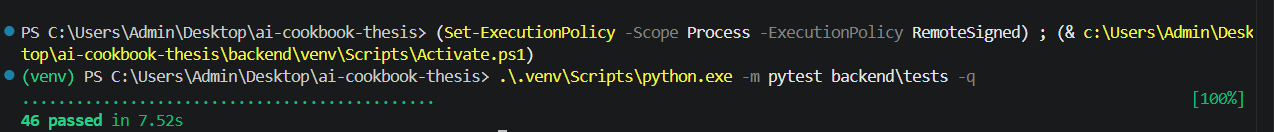
\includegraphics[width=0.9\textwidth]{images/PytestScreenshot.png}
	\caption{Successful backend automated test execution with \texttt{pytest}}
	\label{fig:pytest-suite}
\end{figure}

The executed backend tests are concentrated in four areas:

\begin{itemize}
	\item \textbf{Authentication and authorization:} signup, login, token
	validation, invalid-token rejection, expired-token rejection, and
	protected-route access control.
	\item \textbf{Persistence and user scoping:} saving generated recipes,
	listing recipe history, saving OCR extractions, and ensuring that one
	user cannot see another user's saved content.
	\item \textbf{Validation and preprocessing:} request-schema cleaning,
	image-type checks, image-size limits, and OCR preprocessing rules.
	\item \textbf{Retrieval and orchestration logic:} ingredient conflict
	detection, preference conflict detection, retrieval query formation,
	candidate ranking behavior, and provider selection.
\end{itemize}

The backend evidence covers security, persistence, and intermediate
business logic in addition to basic route responses.

\subsubsection{Frontend automated functional tests}

The frontend test suite was executed with \texttt{Vitest} and the
\texttt{jsdom} environment. These tests validate the behavior of the
React pages and components, including form handling, conditional
rendering, authenticated page states, and structured result display.

The frontend suite completed successfully with \textbf{12 passing tests
across 6 test files}, as shown in
Figure~\ref{fig:vitest-suite}. The tested areas include the login page,
generate-recipe page, saved-recipes page, recipe-history page,
nutrition-label page, and the shared nutrition-grid component.

\begin{figure}[H]
	\centering
	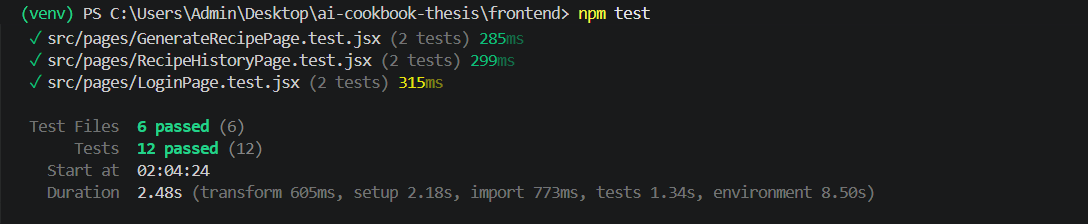
\includegraphics[width=0.9\textwidth]{images/VitestScreenshot.png}
	\caption{Successful frontend automated test execution with \texttt{Vitest}}
	\label{fig:vitest-suite}
\end{figure}

The frontend tests verify several behaviors that are visible to the end
user:

\begin{itemize}
	\item validation errors are shown when required fields are missing,
	\item saved profile defaults are reused correctly during recipe
	generation,
	\item login and profile-update requests are sent with the expected
	payloads,
	\item protected pages display correct guest-only guidance when the user
	is not authenticated,
	\item history entries can be rendered and expanded correctly,
	\item nutrition data is rendered consistently in both recipe and OCR
	contexts.
\end{itemize}

The backend and frontend automated suites provide the main
deterministic correctness evidence for the application.

\subsubsection{Measured test coverage}

In addition to counting passing tests, the executed suites were also
measured for implementation coverage. Backend coverage was measured with
\texttt{coverage.py} over the \texttt{pytest} run, while frontend
coverage was measured with the \texttt{Vitest} V8 coverage provider.
Table~\ref{tab:coverage-summary} summarizes the resulting indicators.

\begin{table}[H]
	\centering
	\small
	\renewcommand{\arraystretch}{1.2}
	\begin{tabularx}{\textwidth}{|p{2.3cm}|p{2.4cm}|p{2.5cm}|>{\raggedright\arraybackslash}X|}
		\hline
		\textbf{Layer} & \textbf{Tool} & \textbf{Metric} & \textbf{Result} \\
		\hline
		Backend & \texttt{coverage.py} + \texttt{pytest} & Statement coverage & \textbf{77\%} overall (1138 of 1474 statements executed). \\
		\hline
		Frontend & \texttt{Vitest} V8 coverage & Statement / line coverage & \textbf{72.98\%} statements and \textbf{74.90\%} lines. \\
		\hline
		Frontend & \texttt{Vitest} V8 coverage & Branch / function coverage & \textbf{55.18\%} branches and \textbf{64.93\%} functions. \\
		\hline
		\end{tabularx}
	\caption{Coverage indicators measured for the automated test suites}
	\label{tab:coverage-summary}
\end{table}

These percentages should be interpreted together with the covered
modules. The backend coverage is strongest in the directly relevant
application layers: \texttt{main.py} reached 100\%, route modules such
as \texttt{auth.py}, \texttt{ocr.py}, and \texttt{recipes.py} reached
98\%, 97\%, and 94\%, \texttt{schemas.py} reached 98\%, and
\texttt{rag\_service.py} reached 91\%. The lower backend totals are
mainly caused by thin provider-adapter and externally dependent modules
such as \texttt{llm\_service.py}, \texttt{ocr\_google\_vision\_provider.py},
\texttt{recipe\_image\_service.py}, and \texttt{vector\_store\_service.py},
which are harder to execute comprehensively in a deterministic local
test environment without turning the thesis suite into a network-
dependent integration harness.

The frontend coverage similarly reflects the actual design of the
application. The most important page-level flows are exercised, but some
secondary branches, especially inside the saved-recipes page, remain
less covered because the current suite prioritizes core navigation,
validation, authenticated state handling, and result rendering over
exhaustive UI edge-case permutation.

\subsubsection{Representative executed test cases}

Table~\ref{tab:representative-test-cases} presents a representative
selection of executed test cases, including the test steps, expected
result, and observed result.

\begin{table}[H]
	\centering
	\scriptsize
	\renewcommand{\arraystretch}{1.2}
	\begin{tabularx}{\textwidth}{|>{\raggedright\arraybackslash}p{1.6cm}|>{\raggedright\arraybackslash}p{2.4cm}|>{\raggedright\arraybackslash}X|>{\raggedright\arraybackslash}X|>{\raggedright\arraybackslash}X|}
		\hline
		\textbf{Layer} & \textbf{Case} & \textbf{Test Steps} & \textbf{Expected Result} & \textbf{Observed Result} \\
		\hline
		Frontend automated & Empty recipe submission validation & Open the Generate page, leave the ingredient field empty, and press \texttt{Generate Recipe}. & A validation error is shown and no API request is sent. & The executed \texttt{Vitest} case rendered the message ``Please enter at least one ingredient'' and confirmed that the mocked API function was not called. \\
		\hline
		Backend automated & Protected profile access without token & Send \texttt{GET /me} without an authorization header. & The endpoint rejects the request with \texttt{401 Unauthorized}. & The executed \texttt{pytest} case returned status code 401, confirming correct protected-route enforcement. \\
		\hline
		Backend automated & Authenticated recipe generation persists history & Generate a recipe as an authenticated user, then request \texttt{/recipes/history}. & The generated recipe is stored and later visible in history with the expected metadata. & The executed backend test verified one history item with the generated identifier, the expected title, and unsaved state metadata. \\
		\hline
		Frontend automated & Saved defaults reused during generation & Render the Generate page for a logged-in user with stored preferences and allergies, enter only ingredients, and submit. & The request payload automatically includes the saved defaults and the page renders a structured recipe response. & The executed \texttt{Vitest} case confirmed both the outgoing payload and the displayed recipe result. \\
		\hline
		Manual scenario & Successful login and account view & Open the Login page, submit valid credentials, and navigate to the Account page. & Authentication succeeds and profile information is displayed. & The executed manual run displayed the account page together with the saved dietary-preference and allergy sections. \\
		\hline
		Manual + OCR evaluation & OCR extraction on a clear nutrition label & Upload \texttt{nutrition-facts.jpg} and execute extraction on the Food Labels page. & Structured nutrition values and raw OCR text are returned without page failure. & The executed case returned calories 257, protein 8\,g, carbohydrates 39.8\,g, fat 9.4\,g, sugar 2.1\,g, sodium 41\,mg, fiber 10\,g, and readable raw OCR output. \\
		\hline
		\end{tabularx}
	\caption{Representative executed test cases with steps, expected result, and observed result}
	\label{tab:representative-test-cases}
\end{table}

\subsection{UI Testing}

\subsubsection{Purpose of screenshot-based UI verification}

Automated frontend tests confirm logic and rendering decisions, but
visual verification was also documented for the main user-facing
workflows. The application contains multiple screens where the
arrangement of controls, messages, cards, and structured outputs is
part of the observed result. Screenshot-based UI verification therefore
documents the implemented pages and the expected sequence of user
actions.

\subsubsection{Main workflow screens}

Figure~\ref{fig:ui-home-login} shows the home page and the
authentication screen. These screenshots document the entry point into
the main workflows and the dedicated authentication view for login and
sign-up.

\begin{figure}[H]
	\centering
	\begin{minipage}{0.48\textwidth}
		\centering
		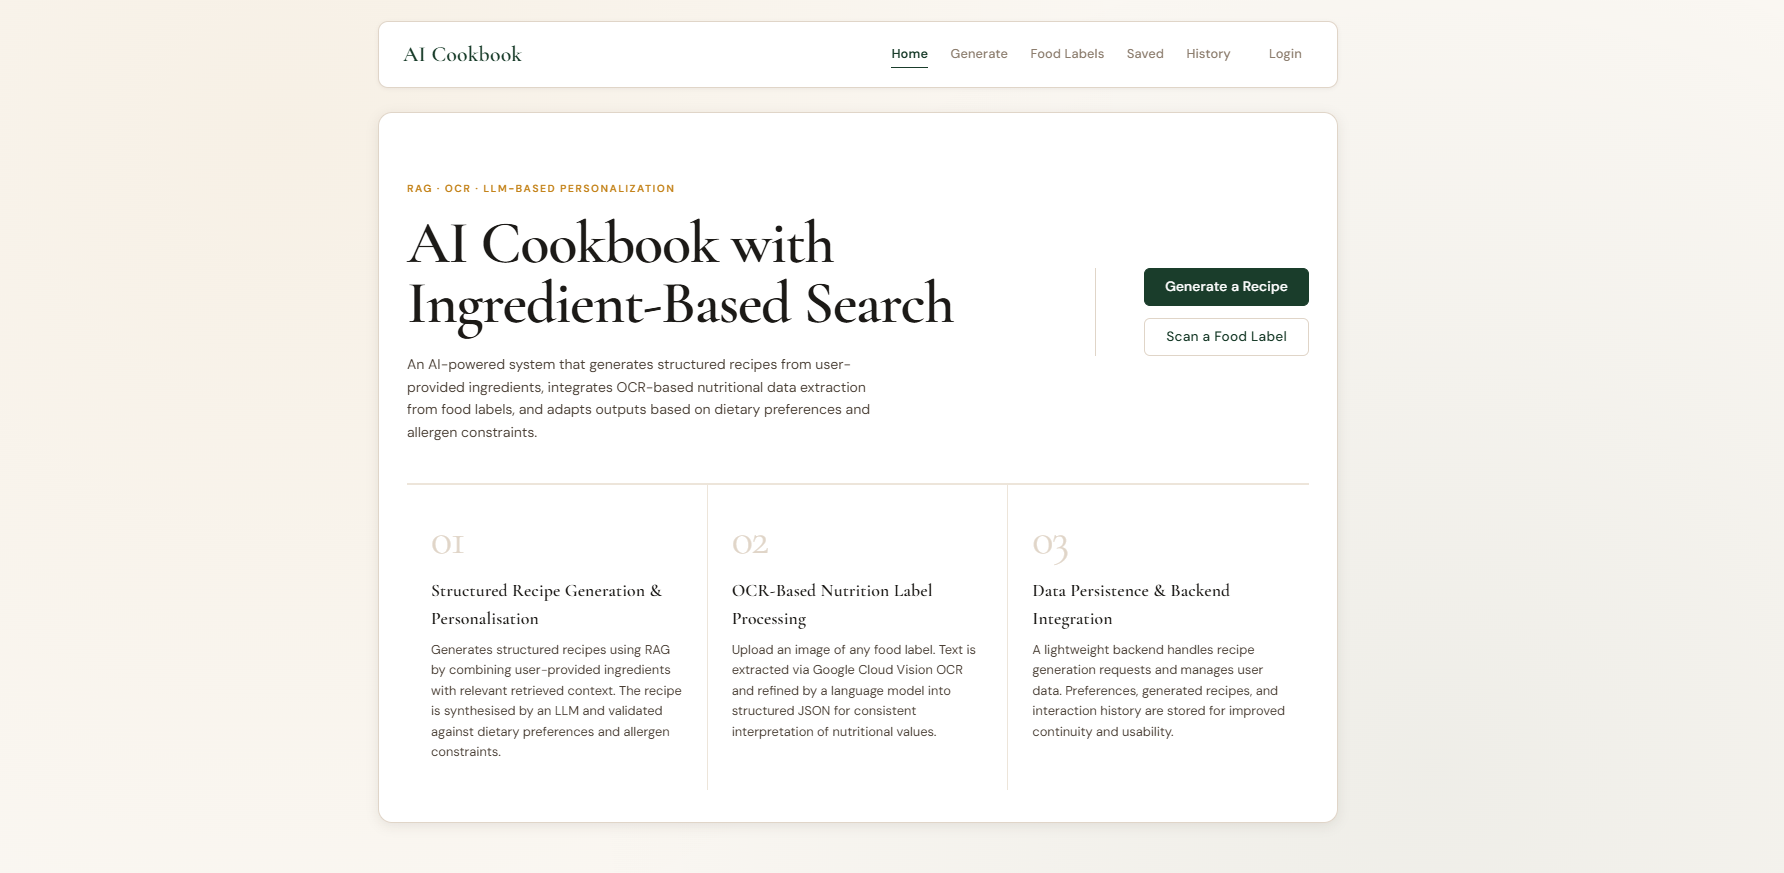
\includegraphics[width=\textwidth]{images/HomePage.png}
		\caption*{(a) Home page}
	\end{minipage}\hfill
	\begin{minipage}{0.48\textwidth}
		\centering
		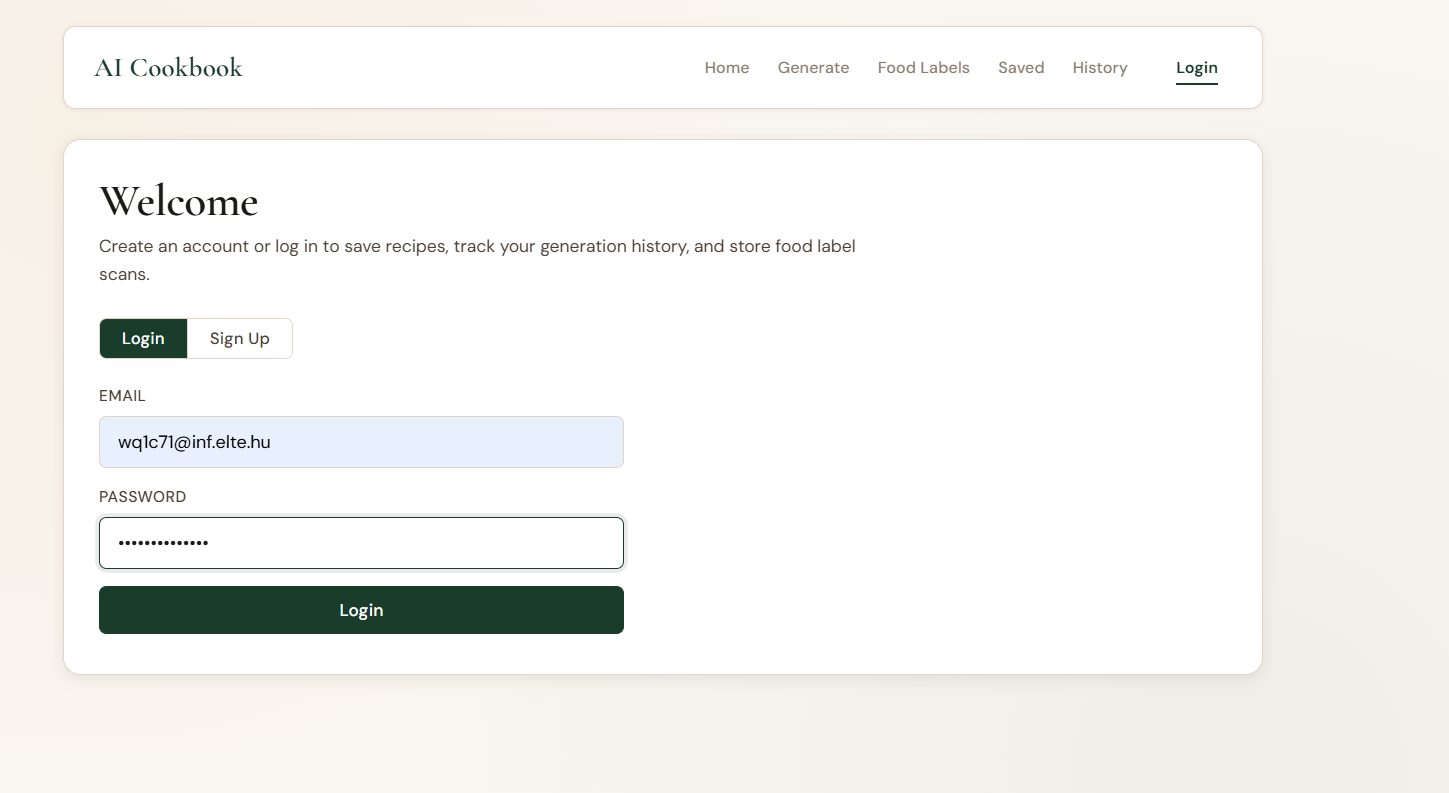
\includegraphics[width=\textwidth]{images/Login.png}
		\caption*{(b) Login and sign-up page}
	\end{minipage}
	\caption{Entry and authentication screens of the implemented frontend}
	\label{fig:ui-home-login}
\end{figure}

Figure~\ref{fig:ui-account-generate} shows the account page and the
recipe-generation page. The account page confirms that user defaults
for dietary preferences and allergies can be viewed and edited, while
the generate page confirms that ingredient input, structured output, and
recipe-specific response presentation are integrated into a single task
flow.

\begin{figure}[H]
	\centering
	\begin{minipage}{0.48\textwidth}
		\centering
		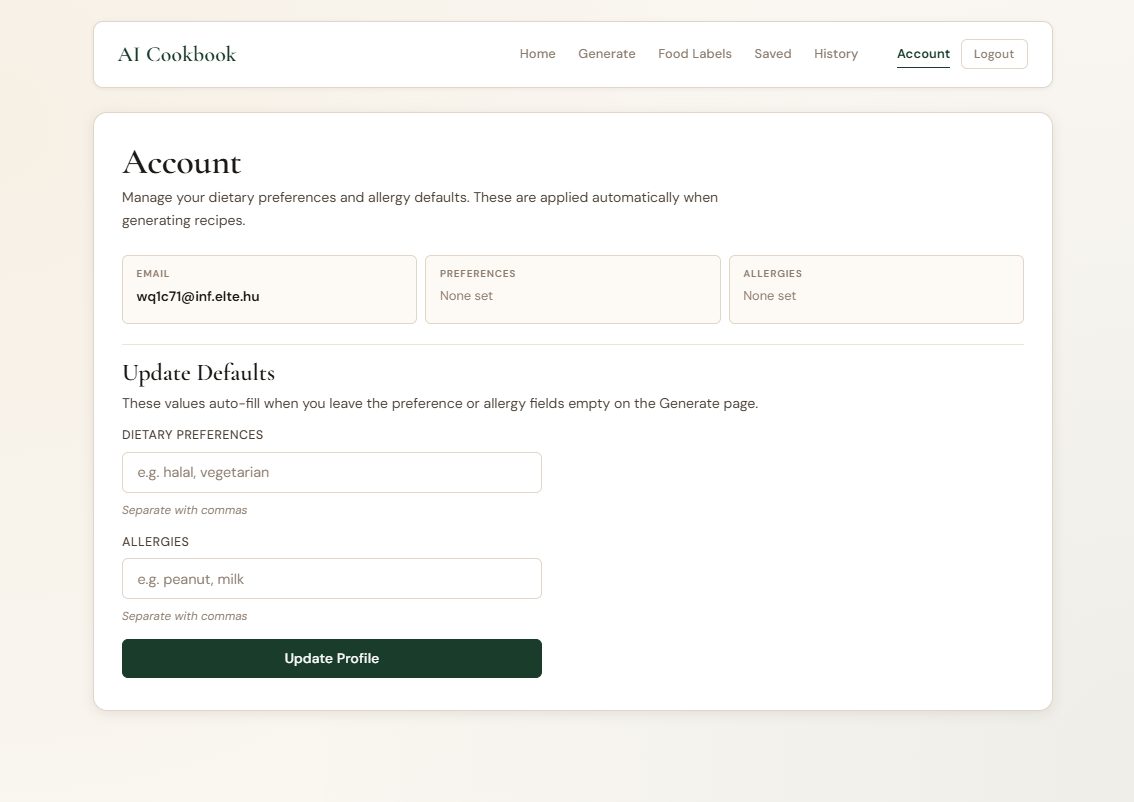
\includegraphics[width=\textwidth]{images/Account.png}
		\caption*{(a) Account and saved defaults}
	\end{minipage}\hfill
	\begin{minipage}{0.48\textwidth}
		\centering
		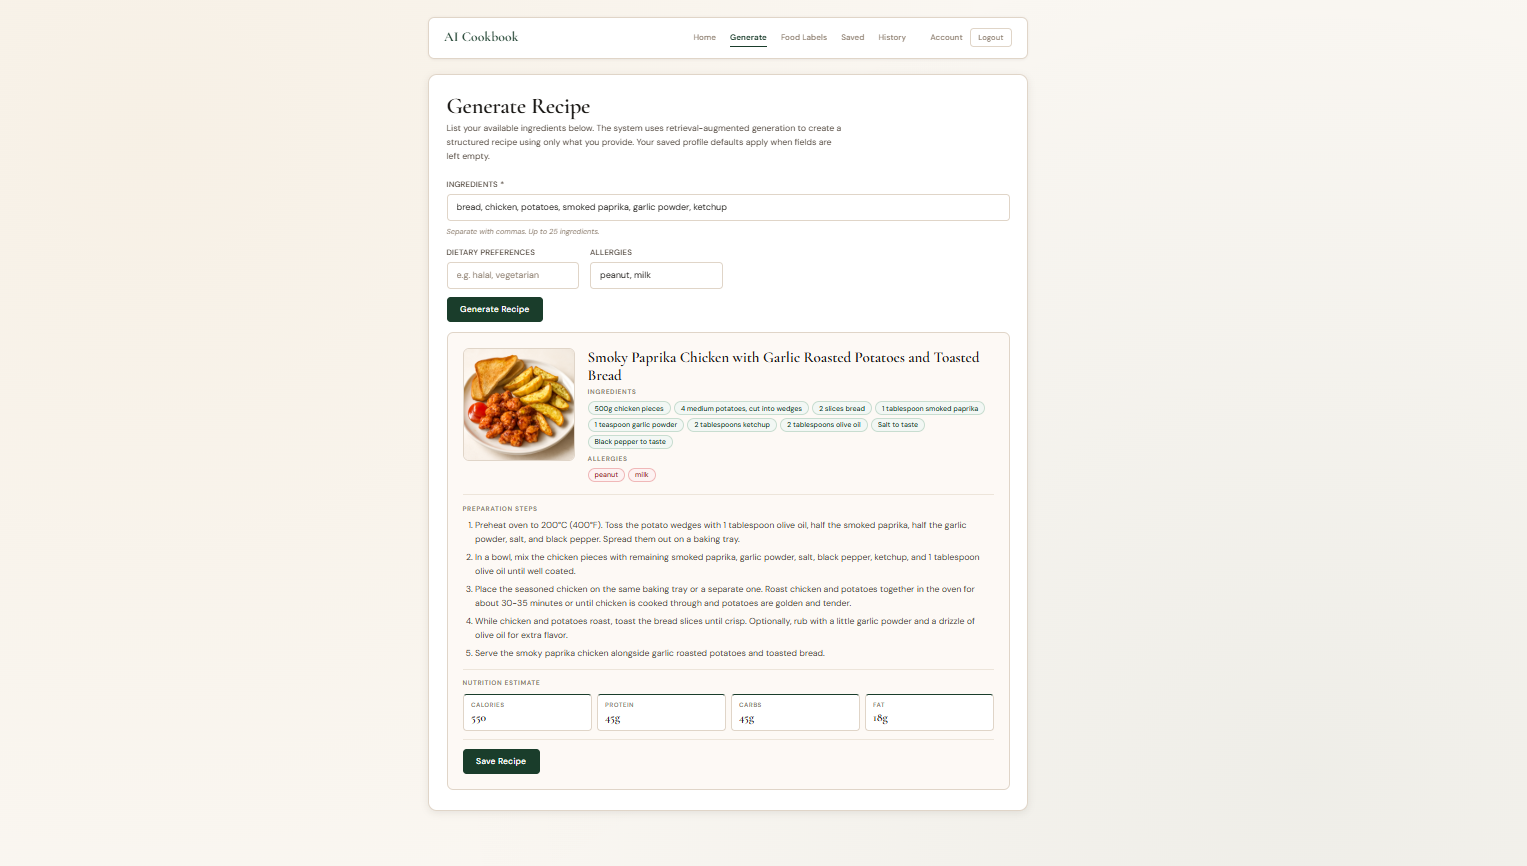
\includegraphics[width=\textwidth]{images/GenerateRecipe.png}
		\caption*{(b) Recipe generation workflow}
	\end{minipage}
	\caption{Authenticated profile management and recipe-generation UI}
	\label{fig:ui-account-generate}
\end{figure}

Figure~\ref{fig:ui-history-saved-ocr} shows the persistence-oriented
screens. These screenshots confirm that generated recipes, explicitly
saved recipes, and OCR nutrition-label processing all have dedicated
presentation flows in the interface.

\begin{figure}[H]
	\centering
	\begin{minipage}{0.32\textwidth}
		\centering
		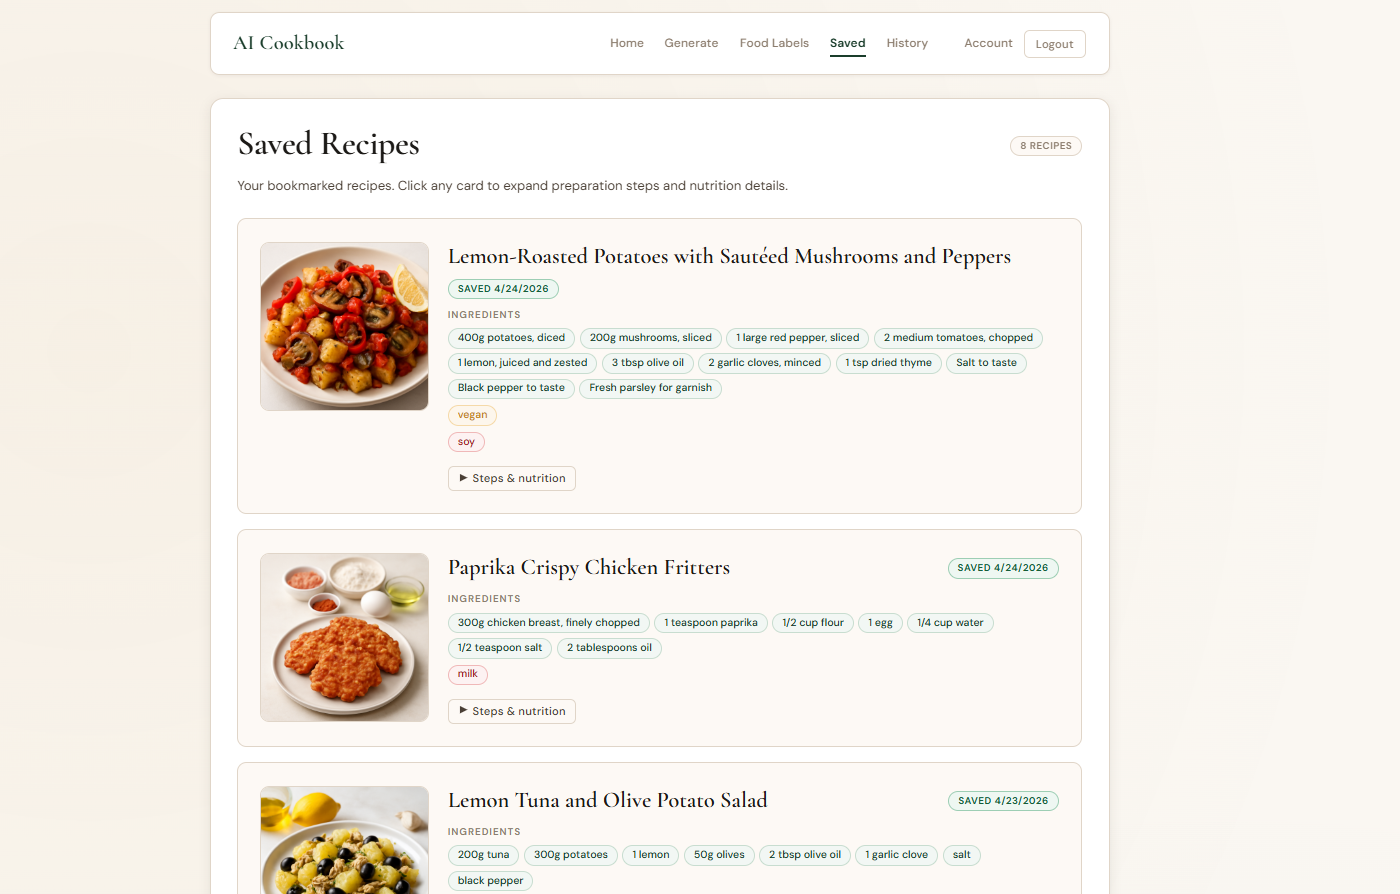
\includegraphics[width=\textwidth]{images/SavedRecipes.png}
		\caption*{(a) Saved recipes}
	\end{minipage}\hfill
	\begin{minipage}{0.32\textwidth}
		\centering
		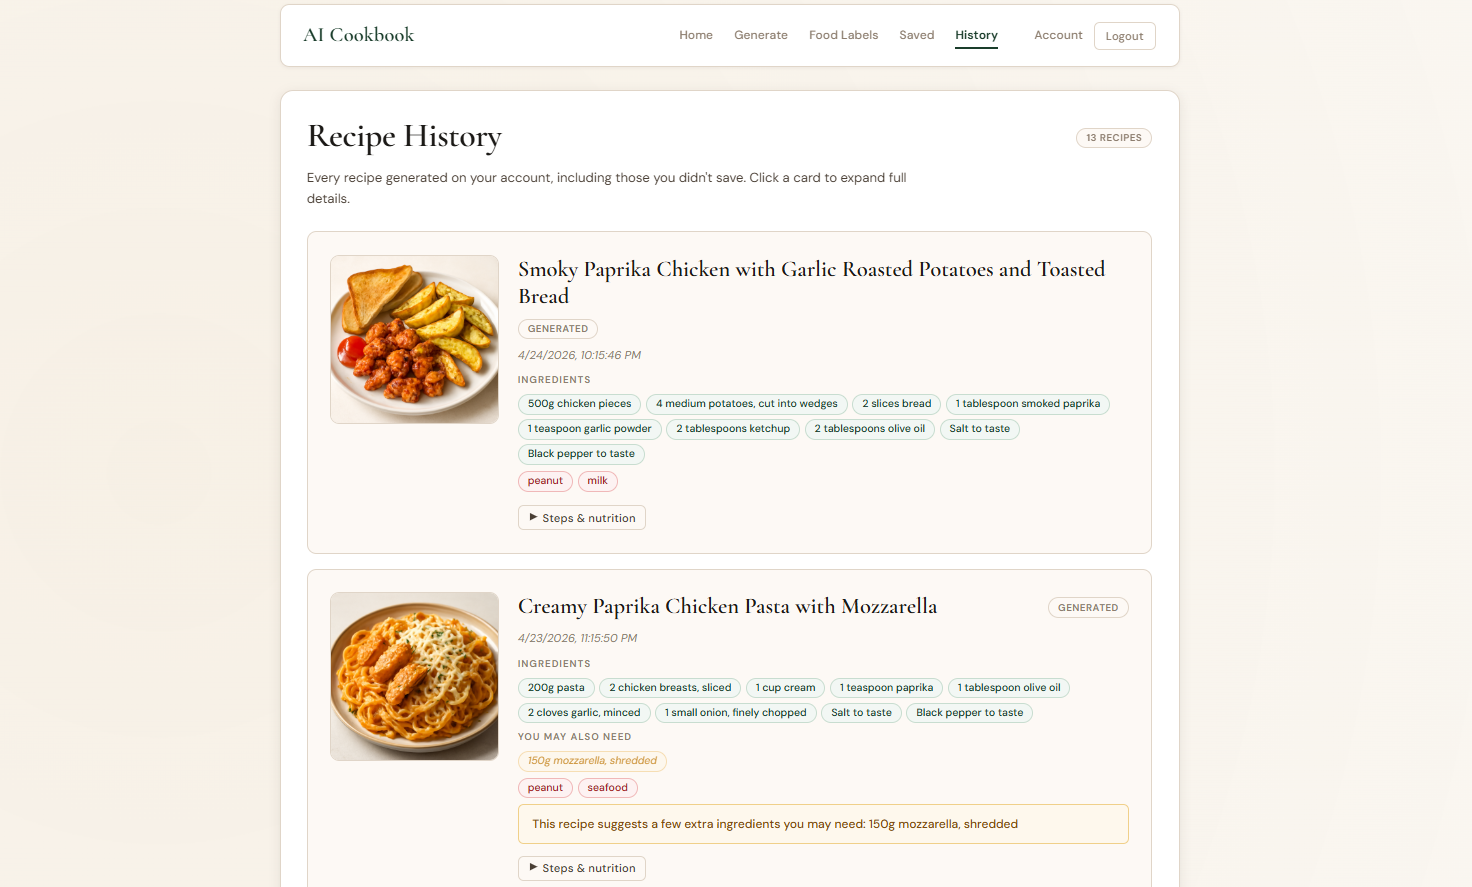
\includegraphics[width=\textwidth]{images/History.png}
		\caption*{(b) Recipe history}
	\end{minipage}\hfill
	\begin{minipage}{0.32\textwidth}
		\centering
		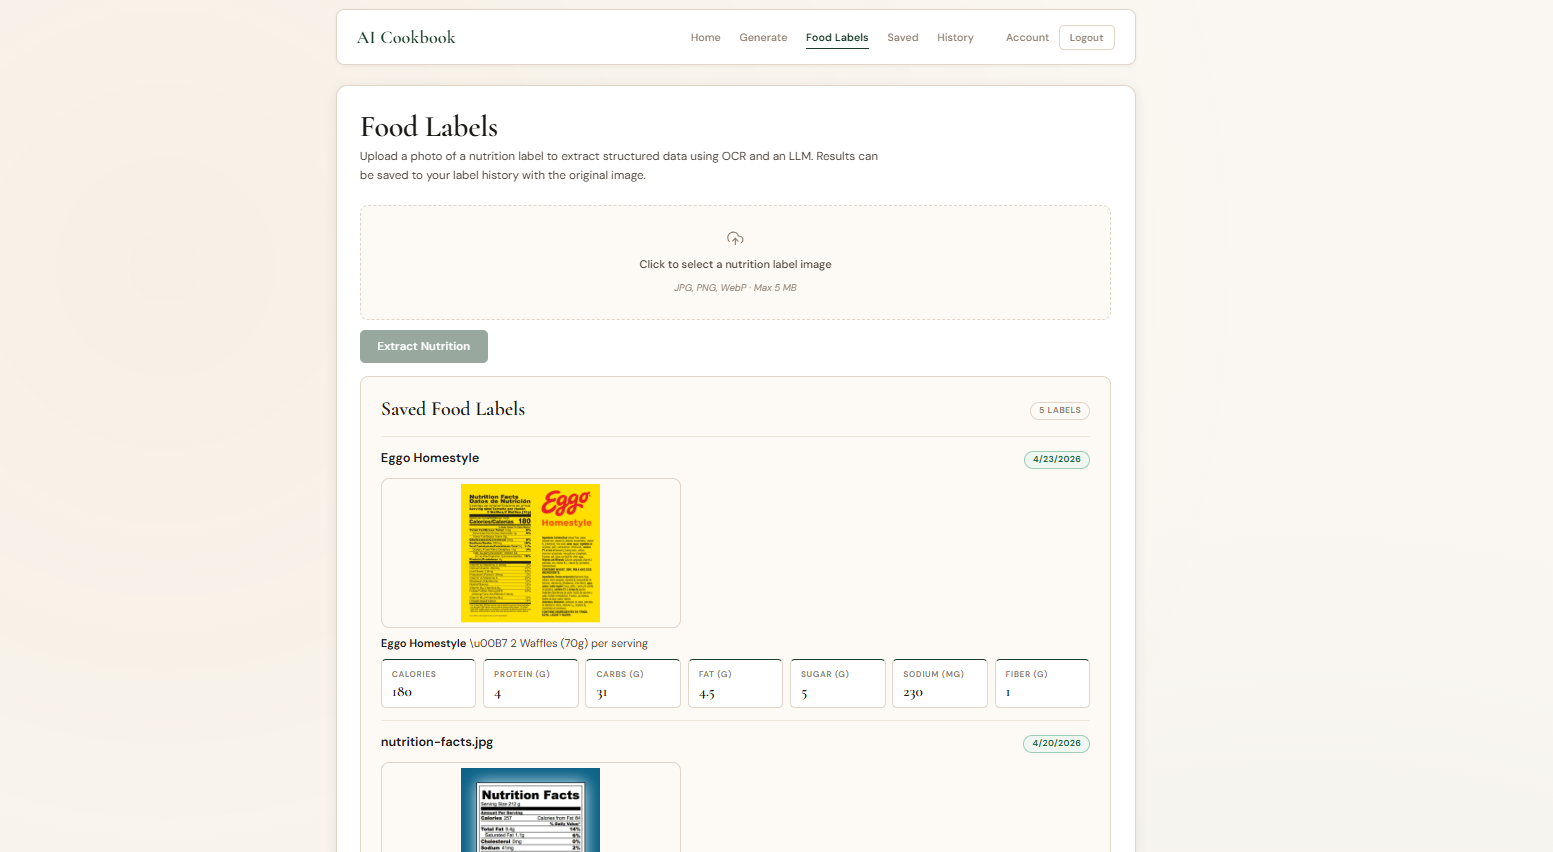
\includegraphics[width=\textwidth]{images/OCR.png}
		\caption*{(c) OCR nutrition-label workflow}
	\end{minipage}
	\caption{Persistence and OCR-related UI screens}
	\label{fig:ui-history-saved-ocr}
\end{figure}

These UI screenshots document three observed properties of the frontend:
the implemented workflows are present, guest and authenticated states
are separated clearly, and the outputs of recipe generation and OCR
extraction are presented in a readable task-oriented format.

\subsection{Integration and End-to-End Testing}

\subsubsection{Postman as API-integration evidence}

To validate the interaction between the HTTP layer, authentication,
backend persistence, and feature-specific routes, the project uses a
dedicated Postman collection. This collection provides request-level
evidence that the implemented API can be exercised outside the frontend
and behaves correctly through direct HTTP calls.

The collection itself is shown in
Figure~\ref{fig:postman-collection}. It documents that the API checks
were organized as a repeatable test set rather than as isolated ad hoc
requests.

\begin{figure}[H]
	\centering
	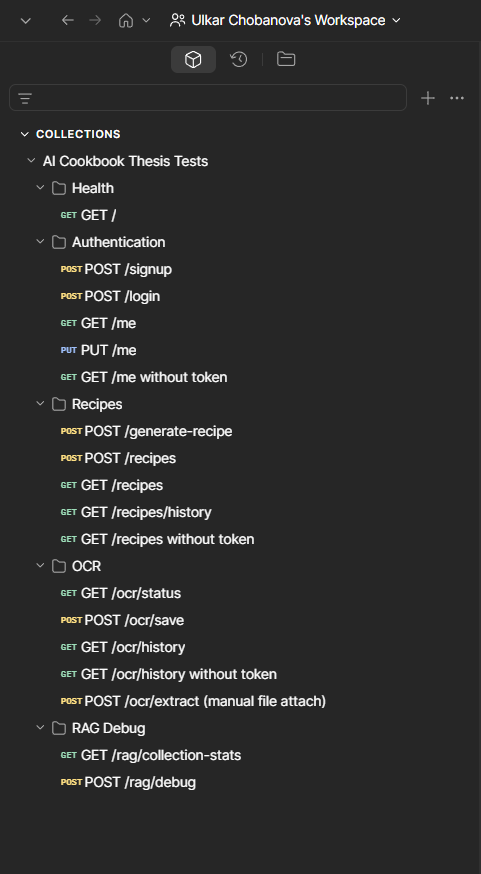
\includegraphics[width=0.82\textwidth]{images/POSTMAN/POSTMANcollection.png}
	\caption{Postman collection used for API-level integration testing}
	\label{fig:postman-collection}
\end{figure}

The Postman checks were executed in a sequence that follows the real
system lifecycle: health verification, account creation, login,
authenticated profile access, main feature calls, persistence actions,
and history retrieval. Figure~\ref{fig:postman-auth} shows the initial
health and authentication requests.

\begin{figure}[H]
	\centering
	\begin{minipage}{0.32\textwidth}
		\centering
		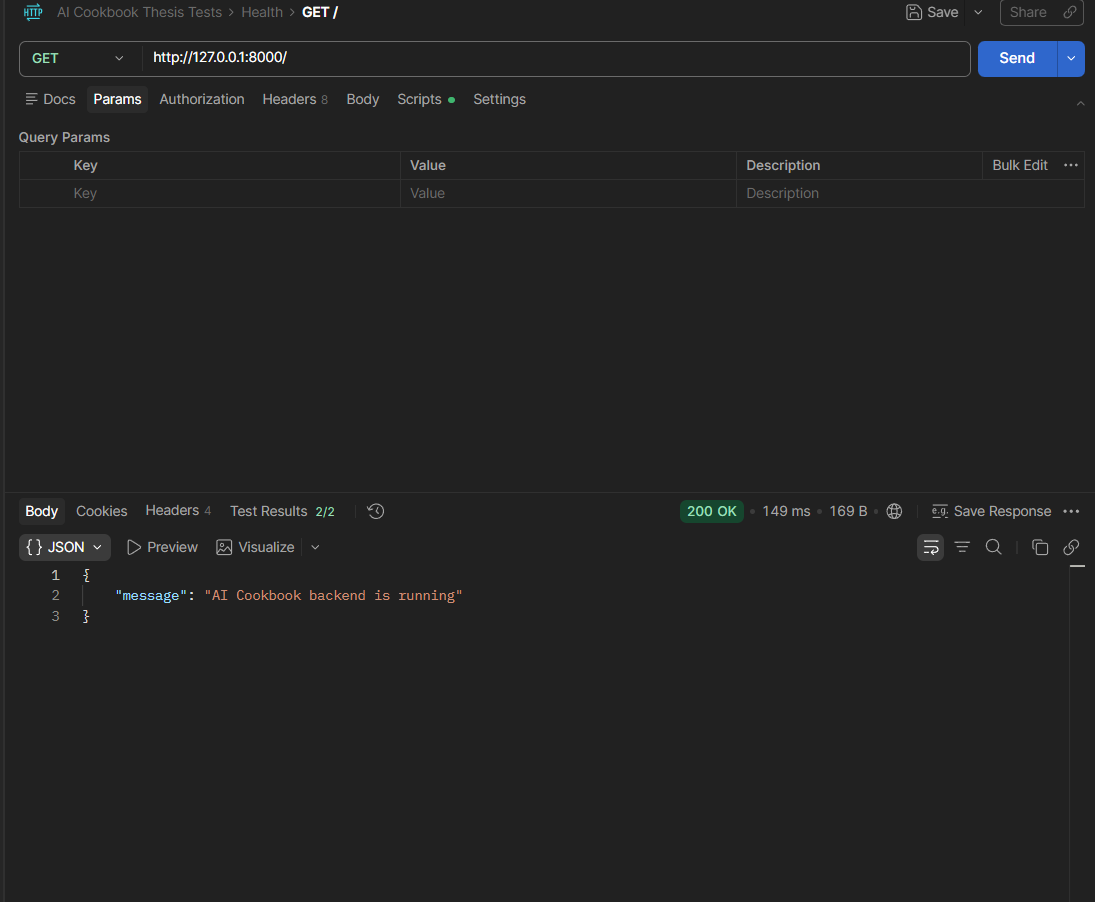
\includegraphics[width=\textwidth]{images/POSTMAN/POSTMANhealth.png}
		\caption*{(a) Health check}
	\end{minipage}\hfill
	\begin{minipage}{0.32\textwidth}
		\centering
		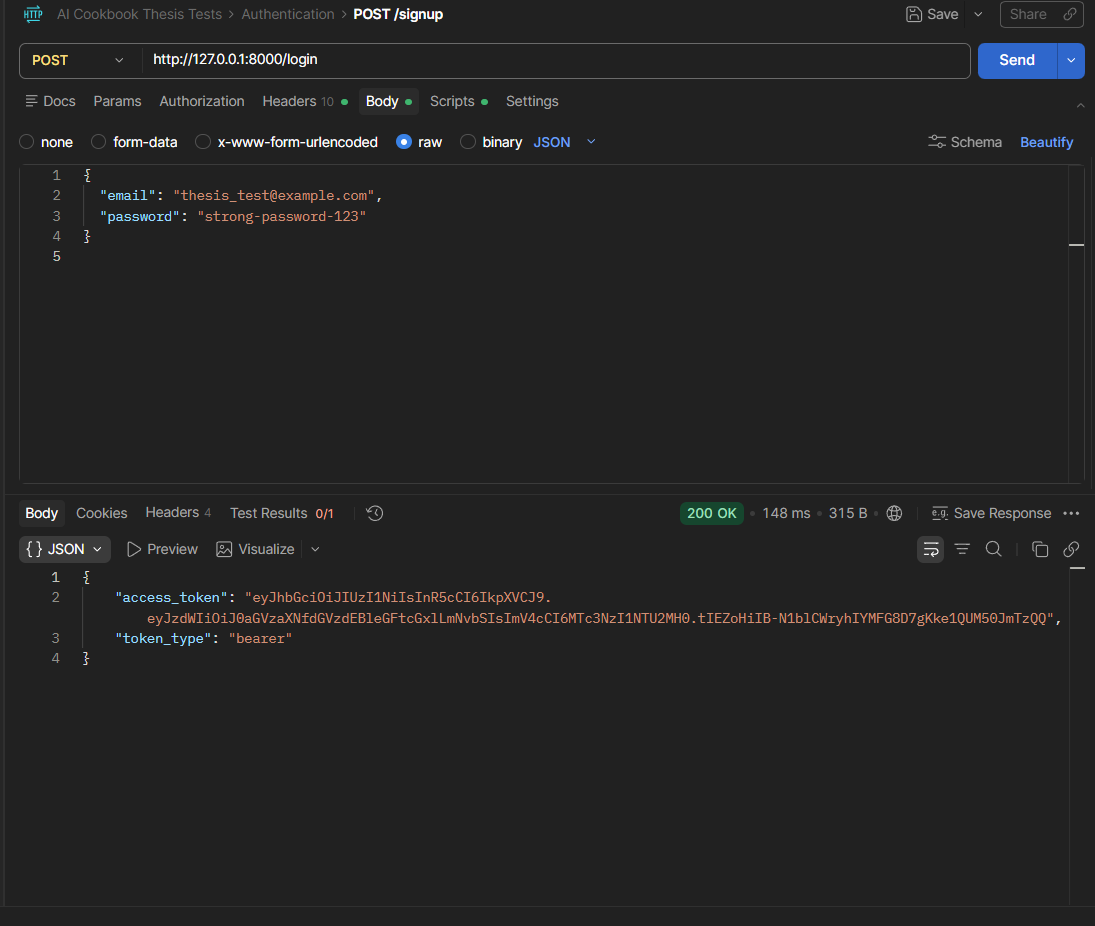
\includegraphics[width=\textwidth]{images/POSTMAN/POSTMANsignup.png}
		\caption*{(b) Signup request}
	\end{minipage}\hfill
	\begin{minipage}{0.32\textwidth}
		\centering
		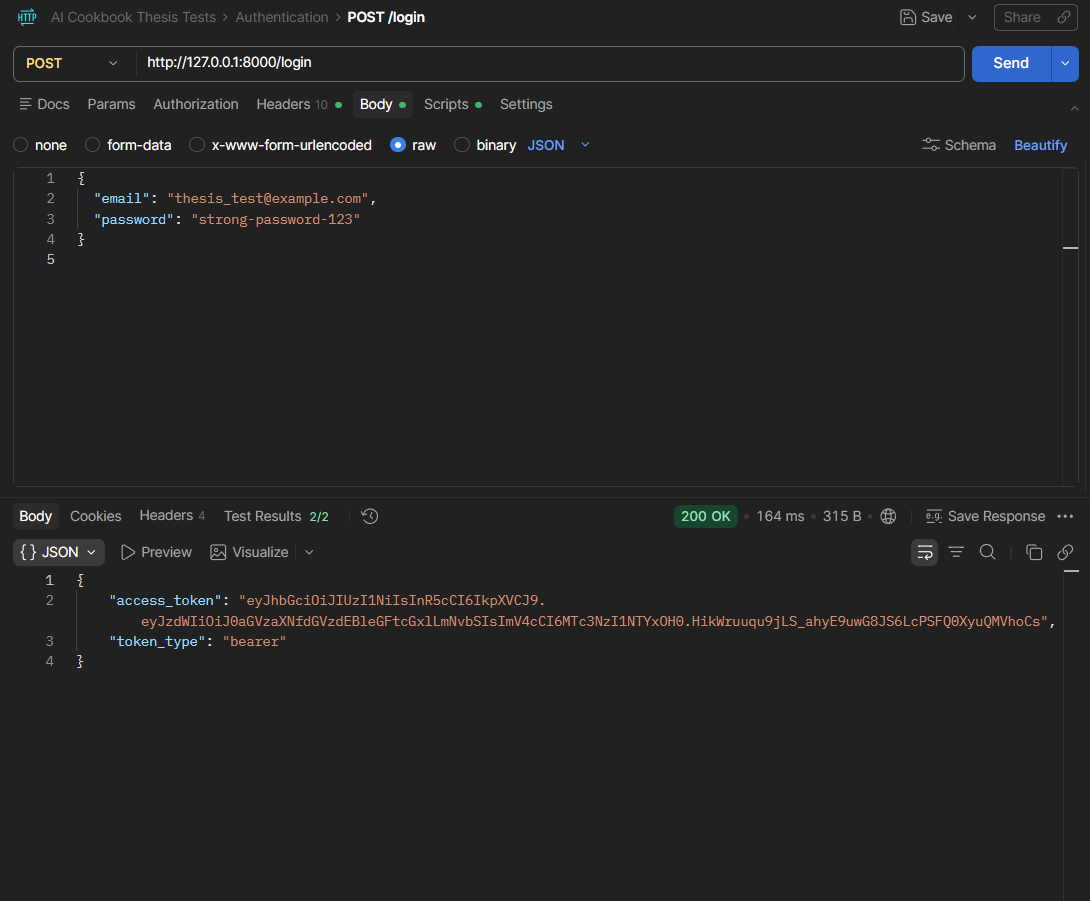
\includegraphics[width=\textwidth]{images/POSTMAN/POSTMANlogin.png}
		\caption*{(c) Login request}
	\end{minipage}
	\caption{Postman evidence for backend availability and authentication}
	\label{fig:postman-auth}
\end{figure}

The health-check response confirms that the backend is running and
reachable. The signup and login responses confirm that account creation
and token issuance work correctly through the public API boundary.

Figure~\ref{fig:postman-protected} shows the profile request and an
unauthorized access attempt. This pair documents both successful
authenticated access and rejection of unauthenticated access to
protected resources.

\begin{figure}[H]
	\centering
	\begin{minipage}{0.48\textwidth}
		\centering
		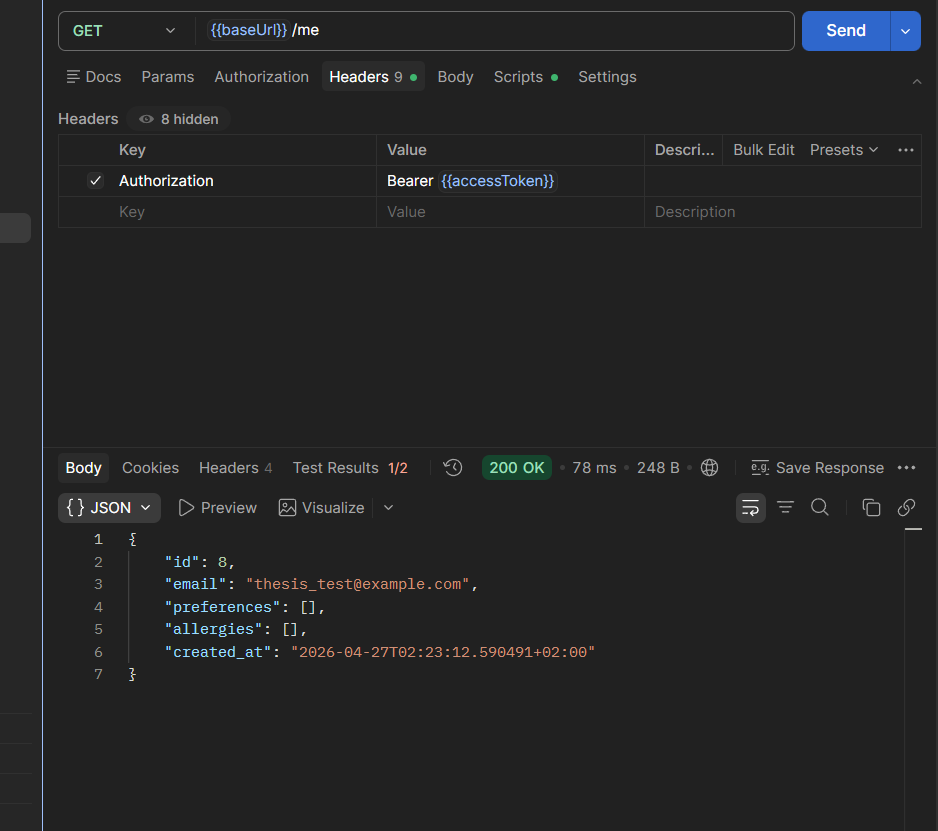
\includegraphics[width=\textwidth]{images/POSTMAN/AuthenticatedProfileRequest.png}
		\caption*{(a) Authenticated \texttt{/me} request}
	\end{minipage}\hfill
	\begin{minipage}{0.48\textwidth}
		\centering
		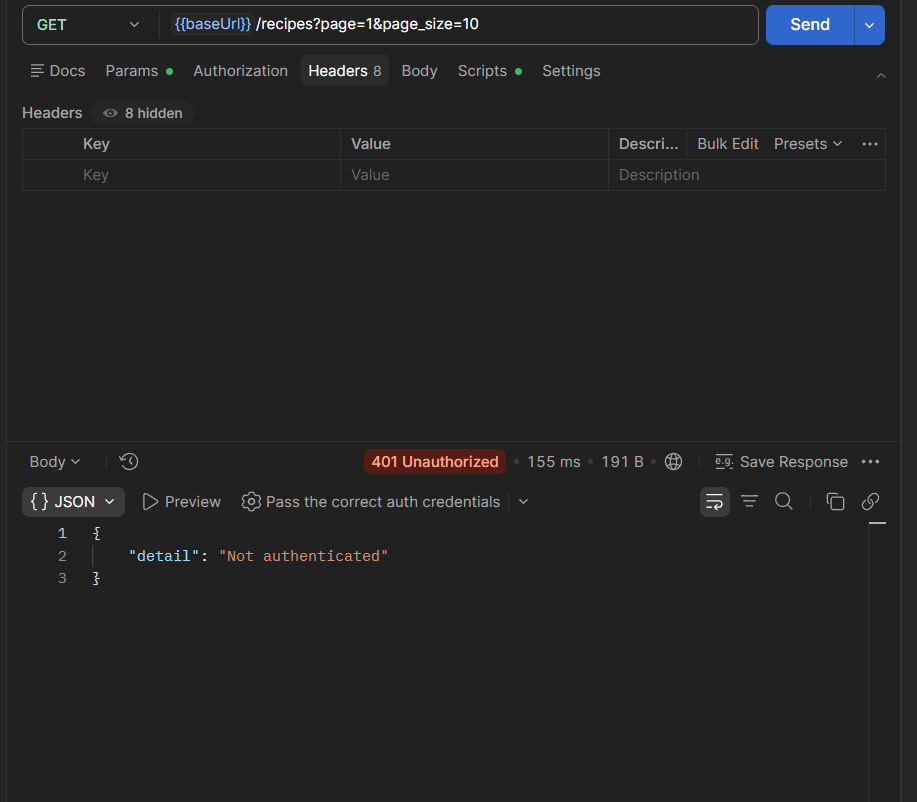
\includegraphics[width=\textwidth]{images/POSTMAN/UnauthorizedProtectedRequest.png}
		\caption*{(b) Unauthorized protected request}
	\end{minipage}
	\caption{Postman evidence for protected-route behavior}
	\label{fig:postman-protected}
\end{figure}

The main recipe-generation integration path is shown in
Figure~\ref{fig:postman-recipe}. The first request demonstrates
successful structured recipe generation through the API. The second
request demonstrates that a generated recipe can then be saved through a
separate persistence endpoint. The third request demonstrates that the
saved or generated item later appears in recipe history.

\begin{figure}[H]
	\centering
	\begin{minipage}{0.32\textwidth}
		\centering
		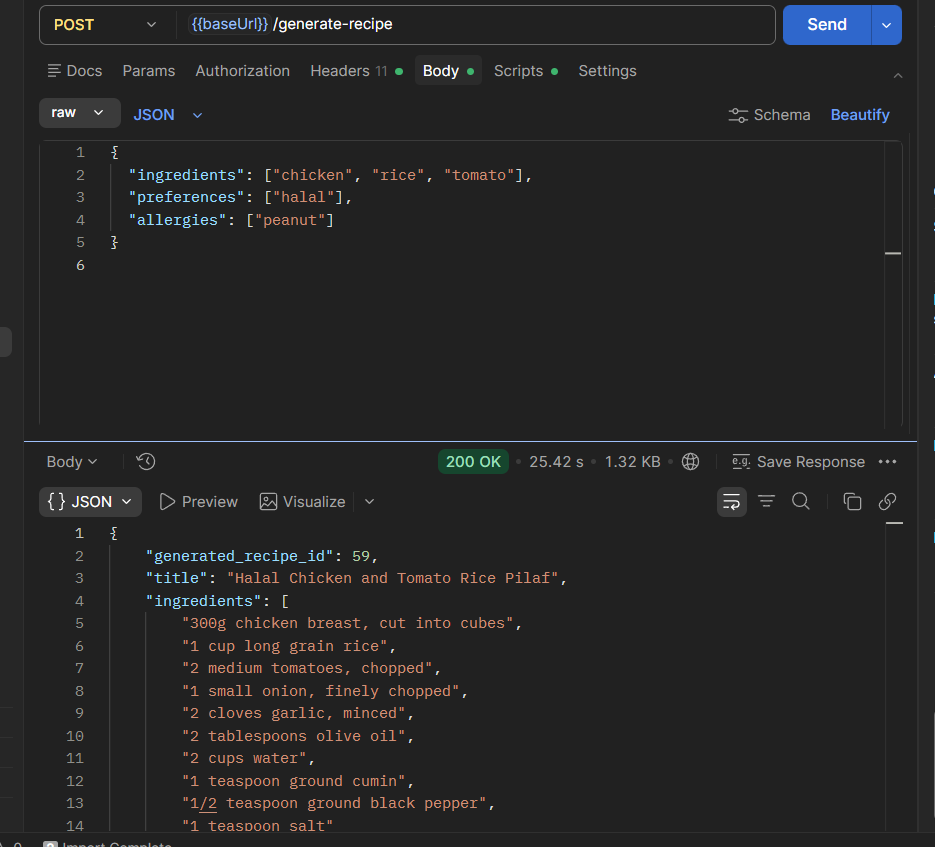
\includegraphics[width=\textwidth]{images/POSTMAN/SuccessfulRecipeGeneration.png}
		\caption*{(a) Recipe generation}
	\end{minipage}\hfill
	\begin{minipage}{0.32\textwidth}
		\centering
		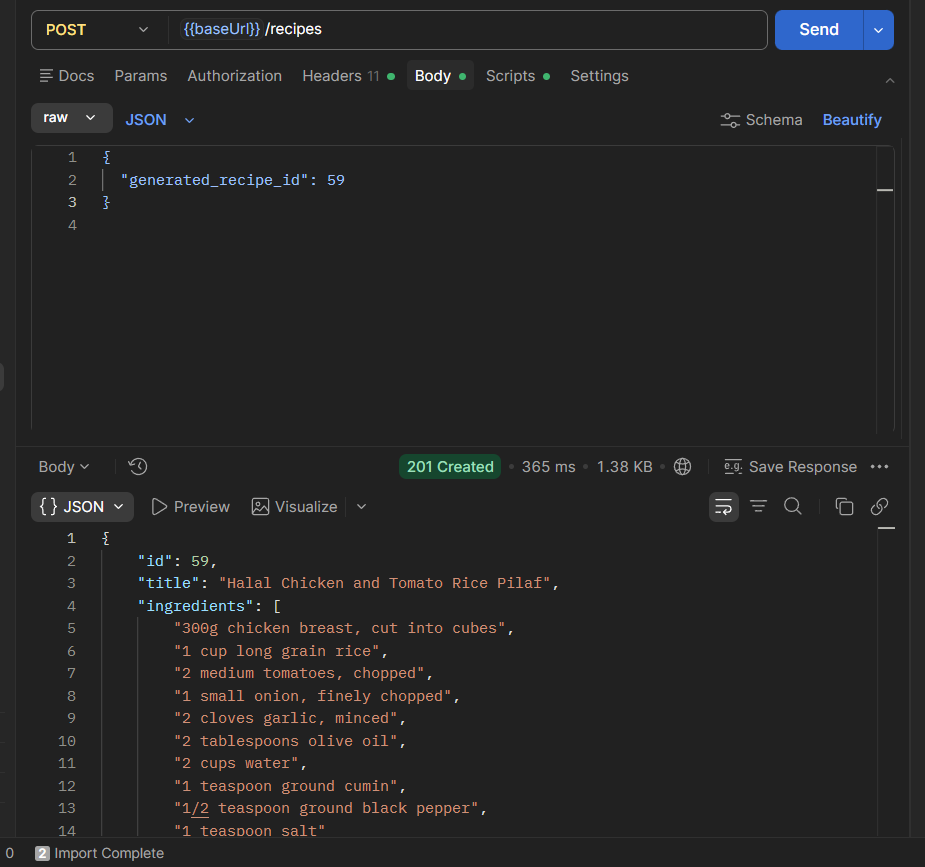
\includegraphics[width=\textwidth]{images/POSTMAN/SaveGeneratedRecipe.png}
		\caption*{(b) Save generated recipe}
	\end{minipage}\hfill
	\begin{minipage}{0.32\textwidth}
		\centering
		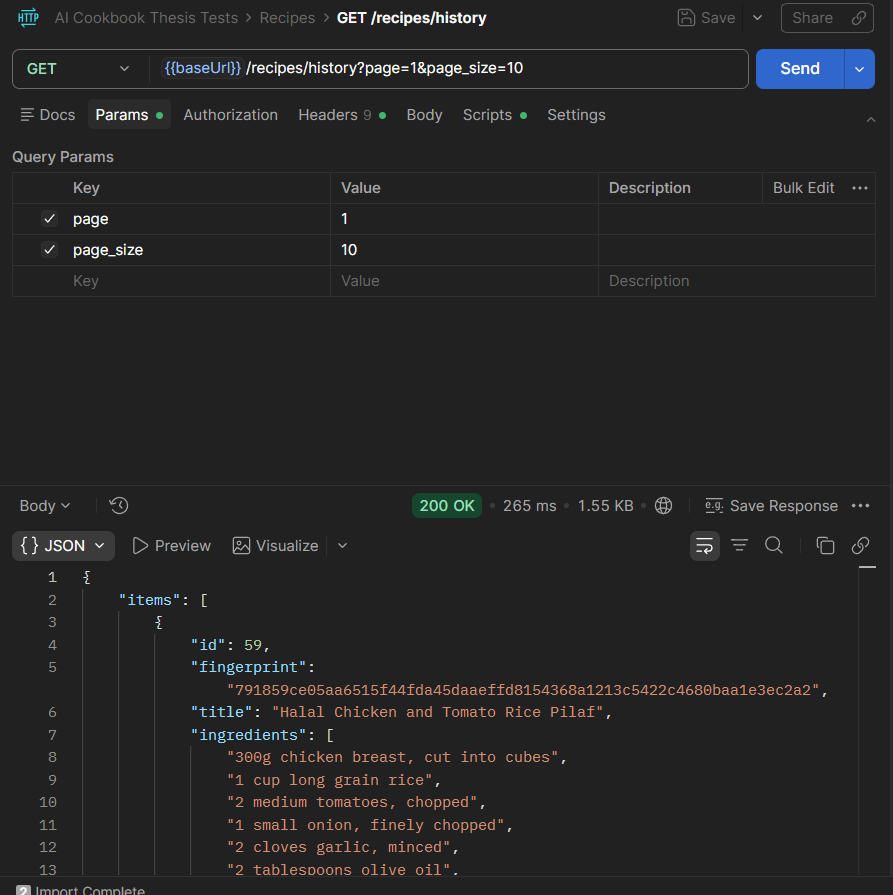
\includegraphics[width=\textwidth]{images/POSTMAN/RecipeHistory.png}
		\caption*{(c) Recipe history retrieval}
	\end{minipage}
	\caption{Postman evidence for recipe-generation and persistence integration}
	\label{fig:postman-recipe}
\end{figure}

This sequence validates a full integration path:

\begin{enumerate}
	\item authenticated user context is accepted,
	\item the recipe-generation endpoint returns structured output,
	\item a generated recipe identifier can be reused by the save endpoint,
	\item the persistence layer stores the record correctly,
	\item the history endpoint returns the stored data through paginated API
	access.
\end{enumerate}

The OCR persistence path is shown in Figure~\ref{fig:postman-ocr}. These
requests confirm that structured OCR-related data can be saved and later
retrieved through the user-scoped history endpoint.

\begin{figure}[H]
	\centering
	\begin{minipage}{0.48\textwidth}
		\centering
		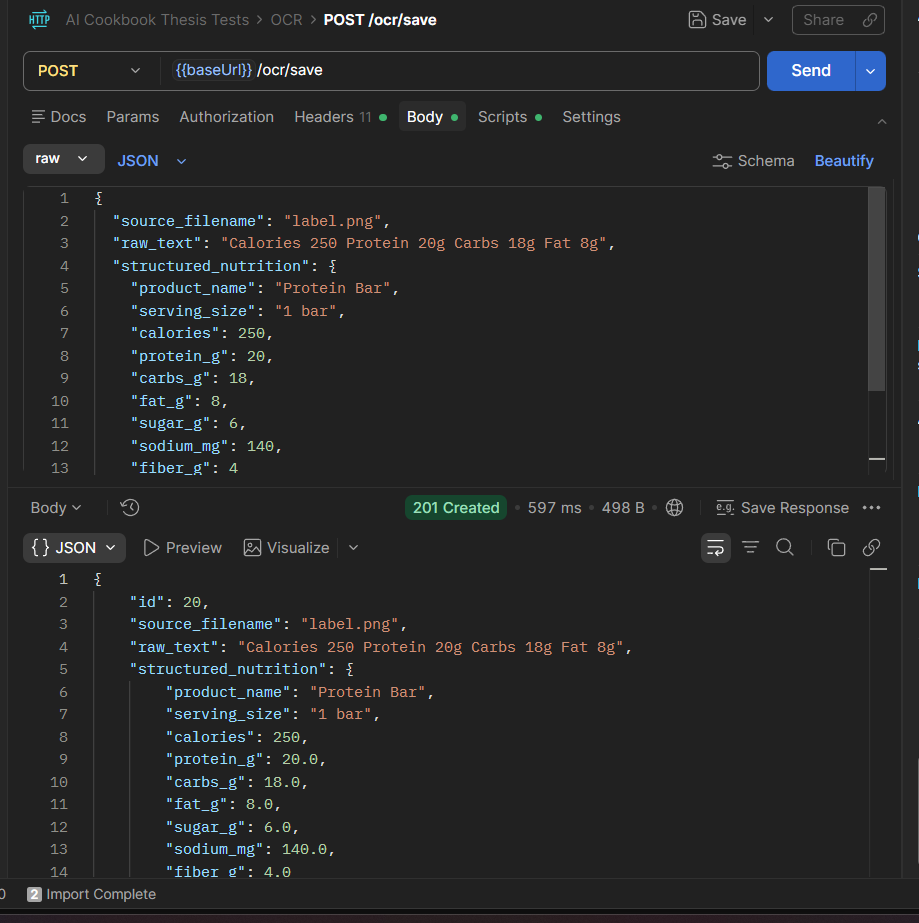
\includegraphics[width=\textwidth]{images/POSTMAN/OCRsave.png}
		\caption*{(a) Save OCR extraction}
	\end{minipage}\hfill
	\begin{minipage}{0.48\textwidth}
		\centering
		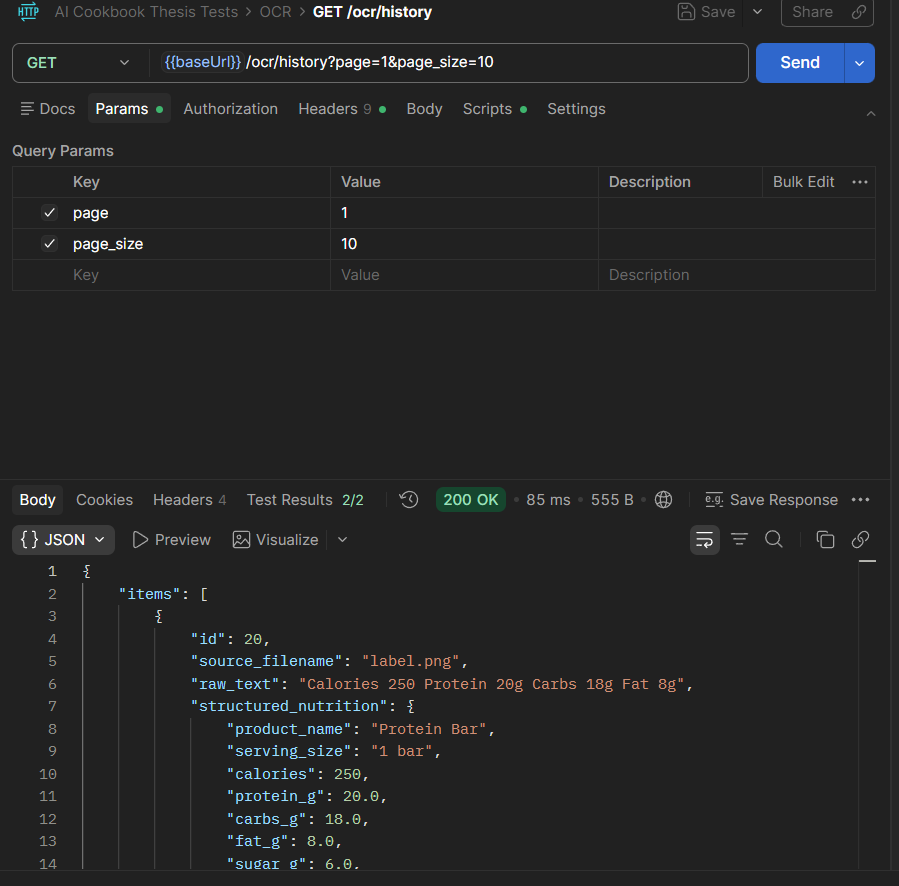
\includegraphics[width=\textwidth]{images/POSTMAN/OCRhistory.png}
		\caption*{(b) OCR history retrieval}
	\end{minipage}
	\caption{Postman evidence for OCR persistence and retrieval}
	\label{fig:postman-ocr}
\end{figure}

Finally, the retrieval subsystem itself is represented by the collection
statistics endpoint shown in Figure~\ref{fig:postman-rag-stats}. This
does not test recipe quality directly, but it does verify that the RAG
layer is implemented as a real subsystem with a persistent collection
and explicit configuration parameters.

\begin{figure}[H]
	\centering
	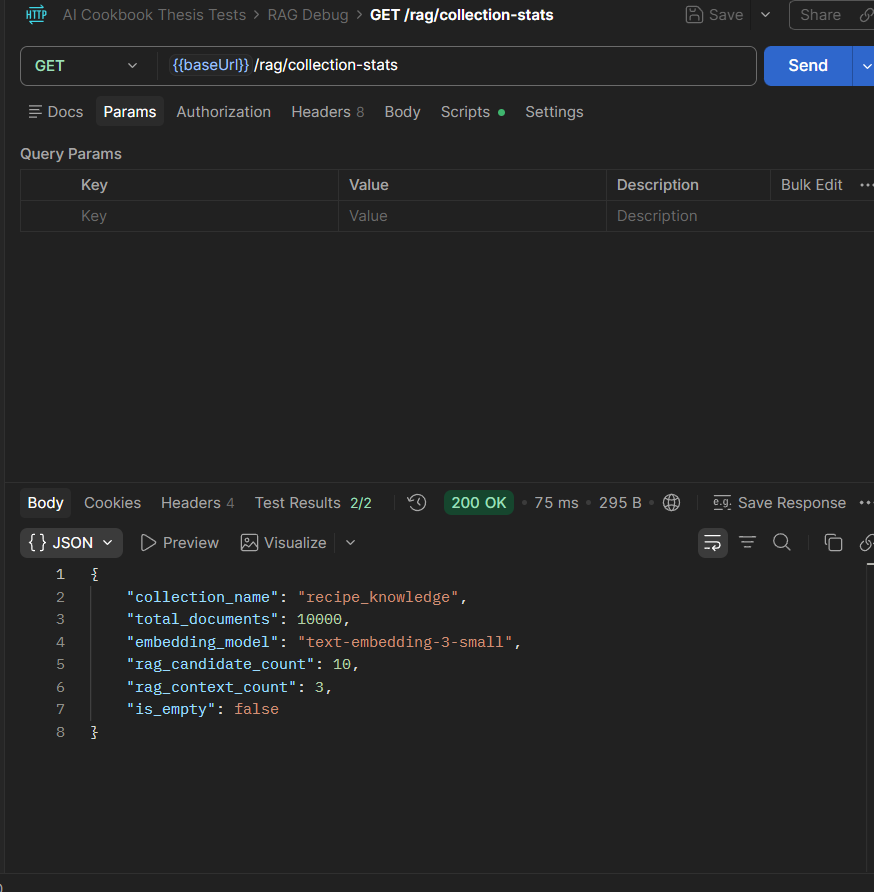
\includegraphics[width=0.78\textwidth]{images/POSTMAN/RAGstats.png}
	\caption{Postman evidence for the retrieval collection statistics endpoint}
	\label{fig:postman-rag-stats}
\end{figure}

Taken together, the Postman evidence validates not just isolated routes,
but real backend integration across authentication, persistence, and
feature-specific workflow boundaries.

\subsection{Advanced Reliability Testing}

\subsubsection{Reliability-oriented backend verification}

In addition to correctness and integration, the backend was also
verified from a reliability perspective. The implemented reliability
tests focus on repeated requests and a small concurrent burst against
the recipe-generation endpoint while external providers are replaced by
deterministic mocks. This approach is appropriate because the project
depends on networked AI services. If those calls were left real during
reliability testing, the results would be dominated by provider latency
and availability rather than the stability of the local application.

The executed reliability-oriented test result is shown in
Figure~\ref{fig:reliability-suite}. The successful run confirms that
the backend can process multiple repeated mocked recipe-generation
requests consistently and can tolerate a small concurrent burst without
failing the internal request path.

\begin{figure}[H]
	\centering
	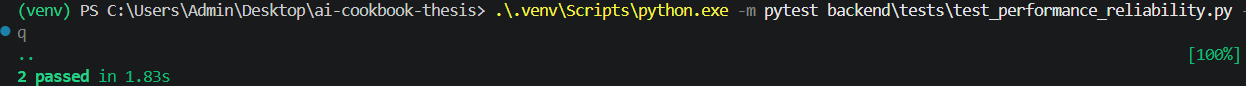
\includegraphics[width=0.9\textwidth]{images/ReliabilityScreenshot.png}
	\caption{Successful reliability-oriented backend test execution}
	\label{fig:reliability-suite}
\end{figure}

This reliability layer should be interpreted carefully. It does
\emph{not} prove real-world latency guarantees for OpenAI or OCR
providers, and it does not replace production load testing. What it
does show is that the internal orchestration of validation, request
handling, and persistence remains stable when the nondeterministic
external dependencies are controlled.

\subsubsection{Role of security-oriented checks}

Security-oriented behavior also appears in the automated and integration
tests. The unauthorized protected-request screenshot in
Figure~\ref{fig:postman-protected} and the backend authentication tests
jointly verify that protected resources are not exposed without a valid
token. The backend rate-limiting tests also validate that repeated
authentication attempts can be restricted at middleware level. For a
project of this scope, this is a meaningful security-oriented testing
layer because it addresses the most relevant risks in the implemented
deployment model: unauthorized access to user-specific saved content and
abusive repeated requests against sensitive endpoints.

\subsection{Manual Scenario-Based Testing}

\subsubsection{Role of manual testing}

Automated backend and frontend tests already confirm a large part of the
deterministic behavior of the application. However, they do not fully
replace scenario-based validation from the perspective of a human user.
Manual testing remains necessary because the project contains
multi-screen workflows that combine authentication state, page
navigation, persistence, generated output display, and OCR result
presentation. These aspects are easier to evaluate coherently when the
system is used as an end user would use it.

For this reason, the project includes a dedicated manual test pack in
\texttt{docs/manual-test-cases.md}. The executed manual cases cover the
main user-facing flows of the application rather than only isolated
controls. The goal of this layer is to confirm that the implemented
features can be completed successfully as end-to-end user tasks and to
support the thesis with screenshot-based evidence.

\subsubsection{Executed manual cases}

The currently executed manual cases cover authentication, profile
management, recipe generation, recipe persistence, history access, OCR
extraction, OCR persistence, and access control. The strongest executed
cases are summarized in Table~\ref{tab:manual-cases-summary}. The table
follows a compact thesis-oriented format similar to classical manual
test documentation: each row identifies the test type, the validated
behavior, the test steps, the expected result, and the observed result.

\begin{table}[H]
	\centering
	\scriptsize
	\renewcommand{\arraystretch}{1.2}
	\begin{tabularx}{\textwidth}{|p{2.2cm}|p{2.0cm}|>{\raggedright\arraybackslash}X|>{\raggedright\arraybackslash}X|>{\raggedright\arraybackslash}X|}
		\hline
		\textbf{Type} & \textbf{Description} & \textbf{Test Steps} & \textbf{Expected Result} & \textbf{Observed Result} \\
		\hline
		\makecell[tl]{UI\\Scenario} & Login page access & Open the frontend, navigate to the Login page, and observe the visible controls. & Login and sign-up tabs are visible, email and password fields are displayed, and the page loads correctly. & The login page loaded successfully and displayed both authentication modes and the required input fields without rendering failure. \\
		\hline
		Functionality & Successful user registration & Open the Login page, switch to Sign Up, enter a valid new email and password, and submit the form. & The account is created successfully, a success message is shown, and the page returns to login mode. & Registration succeeded with valid credentials and the interface returned to the normal authentication flow. \\
		\hline
		Functionality & Successful login and account view & Enter valid user credentials on the Login page, submit the form, and open the Account page. & The user is authenticated successfully and account/profile information is displayed. & The account page displayed the logged-in profile together with the saved preferences and allergies section. \\
		\hline
		\makecell[tl]{Functionality\\Persistence} & Profile default update & Open the Account page, enter dietary preferences and allergies, submit the update form, then refresh or revisit the page. & The profile update succeeds and the new values remain visible after reload. & Updated preference and allergy values remained visible after saving and page revisit, confirming persistence. \\
		\hline
		\makecell[tl]{Functionality\\AI workflow} & Recipe generation with direct input & Open the Generate page, enter a comma-separated ingredient list, and click Generate Recipe. & A structured recipe is returned with title, ingredients, steps, and nutrition estimate, and the page remains stable. & The page returned a complete recipe card and remained stable during response rendering. \\
		\hline
		\makecell[tl]{Functionality\\Personalization} & Recipe generation using saved defaults & Open the Generate page, enter only ingredients, leave preference and allergy fields empty, and generate the recipe. & The stored profile defaults are applied automatically and the generated output reflects those saved constraints. & The generated output reflected the stored personalization settings even though the optional form fields were left blank. \\
		\hline
		\makecell[tl]{Integration\\Persistence} & Save generated recipe & Generate a recipe while logged in, click Save Recipe, then navigate to the Saved page. & The save operation succeeds and the generated recipe appears in the saved recipes list. & The saved recipes page displayed the same recipe after the save action completed. \\
		\hline
		\makecell[tl]{Integration\\Persistence} & Recipe history availability & Generate one or more recipes, open the History page, and inspect the listed entries. & Generated recipes are listed in history, their state is shown, and stored details can be reviewed. & The history page listed the generated entries correctly and allowed their details to be reviewed. \\
		\hline
		\makecell[tl]{Functionality\\OCR} & OCR extraction with valid nutrition label & Open the Food Labels page, upload a valid nutrition-label image, and submit extraction. & The extraction completes successfully and the page displays both raw OCR text and structured nutrition information. & The OCR workflow returned both readable raw text and the expected nutrition field grid for the uploaded label. \\
		\hline
		\makecell[tl]{Integration\\Persistence} & Save OCR extraction & Perform a successful OCR extraction while logged in, save the result, and review the saved label history. & The extraction is stored successfully and appears in the saved OCR history section. & The stored OCR result was later visible in the user-scoped OCR history view. \\
		\hline
		\makecell[tl]{Authentication\\Security} & Protected pages require login & Log out, open the Saved page, then open the History page and observe both responses. & The pages instruct the user to log in and no private saved or historical data is exposed. & Both pages remained inaccessible without authentication and did not expose user-specific content. \\
		\hline
		\makecell[tl]{UI\\Usability} & Expand and collapse saved recipe details & Open the Saved page, expand one saved recipe, then collapse the detail section again. & Steps and nutrition become visible when expanded and are hidden again when collapsed. & The detail section opened and closed correctly while preserving the surrounding page state. \\
		\hline
		\end{tabularx}
	\caption{Manual test cases executed for the AI Cookbook application}
	\label{tab:manual-cases-summary}
\end{table}

The executed manual results show that the application behaves correctly
as a complete user-facing system. Registration and login work in
combination with the account page. Stored preferences and allergies are
reused during recipe generation. Generated recipes can be persisted and
reviewed in the saved-recipes and history views. OCR extraction results
can be produced, saved, and reviewed from history. Protected pages
remain restricted when no authenticated user context is present.

\subsubsection{Relationship to UI and integration testing}

The manual testing layer complements the earlier UI and Postman
sections. UI testing focuses on visible page states and layout-level
evidence. Postman testing focuses on API contracts and HTTP-level
integration. Manual testing documents that a user can complete the full
workflow successfully in the running application.

\subsection{Advanced AI-Related Evaluation}

In addition to deterministic correctness and workflow validation, the
project also includes evaluation of AI-assisted output quality. The
repository therefore contains an evaluation pack for recipe generation
and OCR-based nutrition extraction.

\subsubsection{Recipe-generation evaluation methodology}

The recipe-generation evaluation focuses on the combined behavior of the
RAG retrieval layer, the prompt-driven language-model response, the
restriction-handling logic, and the final structured output returned to
the user. The prepared evaluation cases cover baseline success,
preference satisfaction, allergy filtering, failure handling, and
ingredient drift. Each output was assessed using the following criteria:

\begin{itemize}
	\item \textbf{Structure validity:} whether title, ingredients, steps,
	and nutrition estimate were all present in usable form.
	\item \textbf{Allergy safety:} whether prohibited ingredients were
	successfully excluded or avoided.
	\item \textbf{Preference satisfaction:} whether the generated recipe
	respected the selected dietary rule.
	\item \textbf{Ingredient coverage:} how well the recipe used the
	provided ingredients as its main basis.
	\item \textbf{Additional ingredient count:} how many non-user
	ingredients had to be introduced beyond the basic pantry-like support.
	\item \textbf{Practical quality:} a manual score from 1 to 5 for overall
	usefulness and coherence.
\end{itemize}

\subsubsection{Executed recipe-evaluation results}

Based on the collected recipe outputs, the currently completed
evaluation covers all twelve prepared recipe cases from the repository
worksheet. Eleven of the twelve cases returned a structured recipe
successfully, while one case --- where all provided ingredients
conflicted with the active vegan and milk-avoidance constraints --- was
correctly rejected by the system before unsafe generation could occur.

The aggregated results are summarized in
Table~\ref{tab:recipe-ai-metrics}.

\begin{table}[H]
	\centering
	\scriptsize
	\renewcommand{\arraystretch}{1.2}
	\begin{tabularx}{\textwidth}{|p{4.2cm}|p{2.6cm}|>{\raggedright\arraybackslash}X|}
		\hline
		\textbf{Metric} & \textbf{Value} & \textbf{Interpretation} \\
		\hline
		Total evaluated recipe cases & 12 & Full prepared recipe set was executed. \\
		\hline
		Successful responses & 11 / 12 & Only the fully conflicting input was rejected. \\
		\hline
		Structure validity rate & 91.7\% & Most cases returned complete structured recipe output. \\
		\hline
		Allergy safety rate & 100\% & Allergy-constrained cases stayed safe or were correctly rejected. \\
		\hline
		Preference satisfaction rate & 100\% & Preference-constrained cases respected the declared rule set. \\
		\hline
		Average ingredient coverage score & 0.75 & Most outputs used the provided ingredients well, though conflict-removal cases naturally reduced coverage. \\
		\hline
		Average additional ingredient count & 0.33 & Extra ingredients were generally limited. \\
		\hline
		Average practical quality score & 4.4 / 5 & The outputs were usually coherent and usable in practice. \\
		\hline
		\end{tabularx}
	\caption{Aggregated metrics for recipe-generation AI evaluation}
	\label{tab:recipe-ai-metrics}
\end{table}

The structure validity rate shows that the model usually returns output
in the required application format. The safety and preference metrics
show that the combination of conflict filtering, restriction-aware
prompting, and post-generation validation was effective in the executed
cases. Lower ingredient-coverage scores were expected in cases where
one of the user-provided ingredients conflicted with an allergy or
dietary preference, because the system favored safety over maximal
ingredient reuse.

\subsubsection{Representative recipe-evaluation observations}

The executed outputs also reveal several meaningful qualitative
patterns.

\begin{itemize}
	\item In baseline cases such as vegetarian pasta or simple salad input,
	the generated recipes remained coherent, simple, and strongly centered
	on the user ingredients.
	\item In allergy-constrained cases such as peanut, milk, and shellfish
	avoidance, the system issued explicit warnings and removed the
	conflicting ingredient while still attempting to preserve recipe
	usability.
	\item In preference-conflict cases such as vegetarian input containing
	chicken, the system again preferred rule compliance over preserving the
	conflicting ingredient.
	\item In some simple-input cases, the system suggested one or two extra
	ingredients, which improved practicality but slightly increased
	ingredient drift.
	\item In the fully conflicting case, the system correctly rejected the
	request instead of generating an unsafe or nonsensical output.
\end{itemize}

These observations show that the surrounding rule logic influences the
final quality and safety of the generated result.

\subsubsection{Executed OCR evaluation results}

The OCR-specific evaluation was executed on three representative images:
a clear nutrition label, a different supplement-style label layout, and
a deliberately invalid non-nutrition document. This evaluation measures
whether OCR text is returned and whether the downstream structuring
stage produces correct nutrition fields or rejects unsuitable input.

Table~\ref{tab:ocr-case-summary} summarizes the per-case outcomes. For
the two valid label images, the system extracted all core numeric
nutrition fields correctly. The third case reveals the current failure
mode: the OCR stage successfully read the document text, but the
nutrition-structuring layer still returned a zero-filled nutrition
object instead of rejecting the non-target image as unsupported input.

\begin{table}[H]
		\centering
		\scriptsize
		\renewcommand{\arraystretch}{1.2}
		\begin{tabularx}{\textwidth}{|p{1.15cm}|>{\raggedright\arraybackslash}X|p{1.4cm}|p{1.8cm}|p{1.8cm}|>{\raggedright\arraybackslash}X|}
			\hline
			\textbf{Case} & \textbf{Input type} & \textbf{OCR success} & \textbf{Structured output} & \textbf{Correct fields} & \textbf{Observation} \\
			\hline
			O-01 & Clear nutrition label (\texttt{nutrition-facts.jpg}) & Yes & Yes & 9 / 9 & Serving size and all numeric nutrition values were extracted correctly from the clean label image. \\
			\hline
		O-02 & Alternate supplement-label layout (\texttt{unnamed.jpg}) & Yes & Yes & 9 / 9 & The different visual layout still produced correct serving-size and nutrition values across the core fields. \\
		\hline
		O-03 & Non-nutrition certificate photo (\texttt{WhatsApp Image 2026-04-14 at 13.56.17.jpeg}) & Yes & No & 0 / 9 & OCR text was extracted from the document, but the nutrition layer should have rejected the image instead of returning zero-valued nutrition fields. \\
		\hline
	\end{tabularx}
	\caption{Executed OCR evaluation cases and outcomes}
	\label{tab:ocr-case-summary}
\end{table}

The aggregate OCR metrics are summarized in
Table~\ref{tab:ocr-ai-metrics}. These values show that the OCR pipeline
is strong on valid label images, but still needs a better front-end
screening or classifier step for non-label uploads.

\begin{table}[H]
	\centering
	\scriptsize
	\renewcommand{\arraystretch}{1.2}
	\begin{tabularx}{\textwidth}{|p{4.2cm}|p{2.4cm}|>{\raggedright\arraybackslash}X|}
		\hline
		\textbf{Metric} & \textbf{Value} & \textbf{Interpretation} \\
		\hline
		Total evaluated OCR cases & 3 & Two valid label images and one invalid non-label document were executed. \\
		\hline
		OCR text extraction success rate & 100\% & Text was extracted from all three images, including the invalid document. \\
		\hline
		Structured-output success rate & 66.7\% & Only the two real nutrition-label images produced semantically correct structured nutrition output. \\
		\hline
		Calories exact-match rate & 66.7\% & Calories were correct for both valid labels and incorrect for the invalid document case. \\
		\hline
		Macro-field exact-match rate & 66.7\% & Protein, carbohydrate, fat, sugar, sodium, and fiber fields were correct on the valid labels and failed on the invalid document. \\
		\hline
		Average correctly extracted fields per image & 6.0 / 9 & The strong valid cases are offset by the complete failure of the non-target document case. \\
		\hline
		High-quality extraction share (\(\geq 5\) correct fields) & 66.7\% & Two of the three evaluated images produced practically useful structured results. \\
		\hline
	\end{tabularx}
	\caption{Aggregated metrics for OCR evaluation}
	\label{tab:ocr-ai-metrics}
\end{table}

These OCR results show that the implemented OCR plus structuring
pipeline works well on clear nutrition labels of more than one visual
layout. They also expose a current limitation: the system needs an
explicit rejection rule or document-type classifier before the
nutrition structuring stage, because raw OCR success alone is not
enough to guarantee semantic correctness.

\subsection{Threats to Validity}

The current testing evidence has several limitations that should be
stated explicitly.

\begin{itemize}
	\item External AI providers can change behavior over time, so backend
	correctness does not imply identical future qualitative outputs.
	\item The reliability tests use mocked dependencies and therefore do not
	measure real-world latency of OpenAI or OCR services.
	\item Screenshot-based UI verification demonstrates usability and
	correct rendering, but it is not a substitute for exhaustive browser
	automation across all edge cases.
	\item The manual scenario evidence is strong for the main workflows,
	but it still prioritizes representative end-user tasks over exhaustive
	permutation of every negative and pagination edge case.
	\item The OCR evaluation currently uses only three executed images, so
	its metrics already reveal meaningful behavior, but they should still
	be interpreted as a small-sample evaluation rather than a production-
	scale benchmark.
\end{itemize}

These limitations define the interpretation boundary of the evidence
presented in this chapter.

\subsection{Chapter Summary}

The testing evidence consists of multiple complementary layers.
Automated backend tests verified authentication, persistence,
validation, retrieval support logic, and OCR-related services.
Automated frontend tests verified page behavior and conditional
rendering. Screenshot-based UI verification documented the implemented
user workflows. Postman-based integration checks verified API behavior,
token-based authentication, persistence endpoints, recipe history, OCR
history, and retrieval statistics across component boundaries.
Reliability-oriented backend tests showed stable local request handling
under repeated mocked requests and small bursts. Coverage measurement
showed that the automated suites exercised a large part of the
implemented backend and frontend logic, especially the
security-sensitive and user-visible layers. Manual scenario-based
testing confirmed that the main end-user workflows can be completed in
the running application. AI-specific evaluation showed that recipe
generation performed well across the prepared worksheet and that OCR
worked well on valid labels while still exposing a meaningful failure
mode on non-nutrition input.

The chapter therefore documents both the functional correctness of the
implemented system and the current quality boundary of its AI-assisted
features.

\cleardoublepage

\chapter{Conclusion}
\label{ch:sum}

This thesis presented the design and implementation of an
\emph{AI Cookbook with Ingredient-Based Search}, a web application that
combines personalized recipe generation, OCR-based nutrition-label
processing, and persistent user-specific history. The project was
motivated by two practical problems: deciding what to cook from
available ingredients under dietary constraints, and converting
nutrition-label information from food packaging into structured digital
data without manual transcription.

The final system addresses these problems through a full-stack web
application architecture. Users can submit ingredient lists and receive
structured recipes grounded by retrieval-augmented generation, while
food-label images can be processed through an OCR pipeline that returns
both raw extracted text and structured nutritional fields.
Authenticated users can additionally store dietary defaults, save
generated recipes, and preserve OCR extraction history for later review.

\section{Summary of achieved goals versus original proposal commitments}

The project achieved the main objectives defined in the introduction and
covered the core commitments of the original proposal.

\begin{itemize}
	\item A working recipe-generation workflow was implemented with support
	for ingredients, dietary preferences, allergy constraints, retrieval
	context, warnings, and structured output.
	\item A user account system was implemented with registration, login,
	profile-default storage, recipe history, and saved-recipe support.
	\item An OCR-based nutrition-label workflow was implemented with image
	validation, preprocessing, OCR extraction, structured nutrition
	conversion, and optional persistence.
	\item The system was supported by a real persistence layer, migration
	history, vector retrieval subsystem, and media handling logic.
	\item A multi-layer testing strategy was prepared combining automated
	tests, manual workflow tests, and AI-specific evaluation materials.
\end{itemize}

Taken together, these results show that the final system is a working
application with multiple integrated features rather than an isolated
demonstration of a language-model call.

\section{Lessons learned and challenges encountered}

During the project, the main technical challenge was integrating several
different concerns into one coherent application:

\begin{itemize}
	\item retrieval-augmented generation for recipe personalization,
	\item rule-supported safety filtering for allergies and dietary
	preferences,
	\item OCR combined with language-model-based semantic structuring,
	\item persistence of both classical user data and AI-generated
	content,
	\item a modular architecture separating routes, services, models,
	schemas, and provider abstractions.
\end{itemize}

One of the main lessons learned was that AI-assisted features required
supporting software-engineering structure around them. Validation,
persistence, testing, and explicit limitation handling were necessary
for turning recipe generation and OCR extraction into stable application
features rather than isolated API calls.

Another lesson was that system boundaries had to remain explicit.
External AI providers made output quality and availability partly
dependent on services outside the local application. This affected both
implementation and testing choices, especially for OCR extraction,
recipe generation, and evaluation of output quality.

\section{Current limitations}

Despite the achieved results, the final system still has several
important limitations.

\begin{itemize}
	\item The quality of recipe generation, OCR text extraction, and
	structured nutrition output depends on external AI providers.
	\item The nutritional estimates attached to generated recipes are
	approximate and should not be interpreted as certified dietary
	analysis.
	\item Allergy and dietary handling is safety-oriented but not
	medically complete, since it is based on rule-based filtering and
	prompt-level constraints rather than formal nutritional reasoning.
	\item The default storage and media-serving model is appropriate for
	local thesis deployment, but it is not intended as a final production
	deployment architecture.
	\item The current vector retrieval corpus is intentionally limited in
	scope and therefore cannot represent every culinary style or dietary
	context.
\end{itemize}

These limitations define the boundary between what the system currently
demonstrates and what would still be required for broader real-world
deployment.

\section{Proposed future work and development directions}

The following improvements would be natural continuations of the
project:

\begin{itemize}
	\item Expanding the recipe corpus and improving retrieval quality with
	better metadata and reranking strategies.
	\item Introducing richer user modelling, such as cuisine preferences,
	cooking-time preferences, or meal-type preferences.
	\item Replacing local media storage and process-local rate limiting
	with more deployment-ready infrastructure.
	\item Improving OCR robustness through broader preprocessing options
	and more diverse evaluation datasets.
	\item Extending the nutritional model beyond a small fixed schema
	toward richer product comparison and dietary tracking features.
\end{itemize}

These directions would extend the system beyond the current thesis
scope while building directly on the implemented architecture and
testing results.

\cleardoublepage

% Bibliography (mandatory)
\phantomsection
\addcontentsline{toc}{chapter}{\biblabel}
\nocite{http2022rfc9110,json2017rfc8259,jwt2015rfc7519,foodcom2019kaggle,openai2026platform,openai2026api,openai2026images,openai2026embeddings,google2026vision,fastapi2026docs,pydantic2026docs,pydanticsettings2026docs,sqlalchemy2026docs,alembic2026docs,chromadb2026docs,sqlite2026docs,uvicorn2026docs,httpx2026docs,pillow2026docs,pythondotenv2026docs,pythonjose2026docs,passlib2026docs,argon22026docs,pytest2026docs,coveragepy2026docs,react2026docs,reactrouter2026docs,vite2026docs,vitest2026docs,testinglibraryreact2026docs,testinglibraryjestdom2026docs,jsdom2026docs,postman2026docs,python2026docs,node2026docs,npm2026docs,git2026docs,vscode2026docs,chrome2026docs}
\printbibliography[title=\biblabel]
\cleardoublepage

% List of figures (optional) - useful over 3-5 figures
\phantomsection
\addcontentsline{toc}{chapter}{\lstfigurelabel}
\listoffigures
\cleardoublepage

% List of tables (optional) - useful over 3-5 tables
\phantomsection
\addcontentsline{toc}{chapter}{\lsttablelabel}
\listoftables
\cleardoublepage

% List of codes (optional) - useful over 3-5 code samples
\phantomsection
\addcontentsline{toc}{chapter}{\lstcodelabel}
\lstlistoflistings
\cleardoublepage

% List of symbols (optional)
%\printnomenclature

\end{document}
